\documentclass[xcolor=table, xcolor=dvipsnames]{beamer}\usepackage[]{graphicx}\usepackage[]{color}
%% maxwidth is the original width if it is less than linewidth
%% otherwise use linewidth (to make sure the graphics do not exceed the margin)
\makeatletter
\def\maxwidth{ %
  \ifdim\Gin@nat@width>\linewidth
    \linewidth
  \else
    \Gin@nat@width
  \fi
}
\makeatother


\definecolor{fgcolor}{rgb}{0, 0, 0}
\newcommand{\hlnum}[1]{\textcolor[rgb]{0,0,0}{#1}}
\newcommand{\hlstr}[1]{\textcolor[rgb]{0.545,0.137,0.137}{#1}}
\newcommand{\hlcom}[1]{\textcolor[rgb]{0,0.392,0}{\textit{#1}}}
\newcommand{\hlopt}[1]{\textcolor[rgb]{0,0,0}{#1}}
\newcommand{\hlstd}[1]{\textcolor[rgb]{0,0,0}{#1}}
\newcommand{\hlkwa}[1]{\textcolor[rgb]{1,0,0}{\textbf{#1}}}
\newcommand{\hlkwb}[1]{\textcolor[rgb]{0,0,0}{#1}}
\newcommand{\hlkwc}[1]{\textcolor[rgb]{1,0,1}{#1}}
\newcommand{\hlkwd}[1]{\textcolor[rgb]{0,0,1}{#1}}


\usepackage{framed}
\makeatletter
\newenvironment{kframe}{%
 \def\at@end@of@kframe{}%
 \ifinner\ifhmode%
  \def\at@end@of@kframe{\end{minipage}}%
  \begin{minipage}{\columnwidth}%
 \fi\fi%
 \def\FrameCommand##1{\hskip\@totalleftmargin \hskip-\fboxsep
 \colorbox{shadecolor}{##1}\hskip-\fboxsep
     % There is no \\@totalrightmargin, so:
     \hskip-\linewidth \hskip-\@totalleftmargin \hskip\columnwidth}%
 \MakeFramed {\advance\hsize-\width
   \@totalleftmargin\z@ \linewidth\hsize
   \@setminipage}}%
 {\par\unskip\endMakeFramed%
 \at@end@of@kframe}
\makeatother

\definecolor{shadecolor}{rgb}{.97, .97, .97}
\definecolor{messagecolor}{rgb}{0, 0, 0}
\definecolor{warningcolor}{rgb}{1, 0, 1}
\definecolor{errorcolor}{rgb}{1, 0, 0}
\newenvironment{knitrout}{}{} % an empty environment to be redefined in TeX

\usepackage{alltt} % , handout, draft
\usetheme{Madrid} % Madrid, Warsaw, Berlin
\usecolortheme{beaver}

\usepackage[latin1]{inputenc} % windows
%\usepackage[utf8]{inputenc} %linux
\usepackage[T1]{fontenc} % for textbackslash
\usepackage[german, english]{babel}
\usepackage{natbib} % bibliography issues. cite in a scientific way
\usepackage{rotating} % rotate tables pictures..
\usepackage{float} % placing floats (table and figures) at exactly the place i want them to
\usepackage{lmodern} % warnings disappear within the beamer class
\usepackage[capitalise, noabbrev]{cleveref} % smart referencing
\usepackage{colortbl, tabu, multirow} % For coloring table rows and text inside them
\usepackage[labelfont=scriptsize, font=scriptsize]{caption}
\usepackage{url, hyperref, textcomp, amsmath, listings, datetime, graphicx, booktabs, xcolor}
%\usepackage{booktabs} % for thick lines in tables
%\usepackage{wasysym, breakurl}

\hypersetup{pdfstartview={XYZ null null 1}}
\hypersetup{colorlinks=true, linkcolor=blue, urlcolor=blue}


\setbeamertemplate{footline}[text line]{%
  \parbox{\linewidth}{\vspace*{-8pt}\hfill \hyperlink{toc}{TOC} ~~ \insertframenumber / \inserttotalframenumber~~~~~~~~~}}
\setbeamertemplate{navigation symbols}[only frame symbol]

\beamersetleftmargin{0.3cm}
\beamersetrightmargin{0.3cm}



% Reduce spacing in table of contents (toc) http://tex.stackexchange.com/questions/51452
\usepackage{etoolbox}
\makeatletter
\patchcmd{\beamer@sectionintoc}{\vskip1.5em}{\vskip0.1em}{}{} % vskip0.5em
\makeatother

% white letters in enumerate bullet points
\setbeamercolor{item projected}{fg=white}%fg=blue,bg=red!75!black} % fg=white
% Block title color
\setbeamercolor{block title}{fg=white}%fg=blue,bg=red!75!black} % white


% define an environment for the exercises
\newcounter{exercisecount}
\setcounter{exercisecount}{0}
\newenvironment{exercise}[1]
{% This is the begin code
\stepcounter{exercisecount} 
\begin{block}{Exercise \arabic{exercisecount}: #1}
}
{% This is the end code
\end{block} }


% format inline R command names in blue courier:
\newcommand{\rcode}[1]{\texttt{\textcolor{Blue}{#1}}} % or use Blue


% Table of data and object types, with higlighted rows
\newcommand{\datatypes}[9]{
\begin{frame}\frametitle{Data types}
\begin{center}
\begin{tabu}{| l | l | l | l |}   \hline                        
                \textbf{Description}  & \textbf{example}     &\textbf{\rcode{typeof}} &\textbf{\rcode{class}} \\\hline  \hline
\rowfont{\color{#1}} integer number   & 4:6                  & integer   & integer   \\ \hline 
\rowfont{\color{#2}} decimal          & 8.7                  & double    & numeric   \\ \hline
\rowfont{\color{#3}} character string & "homer rocks"        & character & character \\ \hline
\rowfont{\color{#4}} category         & factor("left")       & integer   & factor    \\ \hline
\rowfont{\color{#5}} complex          & 5+3i                 & complex   & complex   \\ \hline
\rowfont{\color{#6}} logical          & c(T, F, FALSE, TRUE) & logical   & logical   \\ \hline
\rowfont{\color{#7}} not available    & NA                   & logical   & logical   \\ \hline
\rowfont{\color{#8}} empty set        & NULL                 & NULL      & NULL      \\
  \hline  
\end{tabu}
\end{center}
\color{#9}
%See also e.g. Uwe Ligges (2006) - Programmieren mit R\\
\rcode{as.character}\texttt{(3.14)} converts a data type;  \rcode{is.integer}\texttt{(4:6)} checks.
\rcode{str} shows an abbreviaton of \rcode{class}.\\
\rcode{mode} (for users) is like \rcode{typeof} (R internal), but combines integer and double to numeric (VeryAdvanced: also combines closure, special and builtin to function). Other rare typeofs: raw, environment, promise, ...
\end{frame}
}

\newcommand{\objecttypes}[7]{
\begin{frame}\frametitle{Object types}
\begin{center}
%\begin{tabu}{| l | m{4cm} | m{3cm} | l |}  \hline  
\begin{tabu}{| l | l | l | l |}  \hline 
    \textbf{Object} & \textbf{example}                    &  \textbf{\rcode{typeof}} & \textbf{\rcode{class}}\\ \hline   \hline  
\rowfont{\color{#1}} vector    & see data types                            & data type           & data type  \\ \hline
\rowfont{\color{#2}} matrix    & matrix(9:15, ncol=2)                      & integer   & matrix     \\ \hline
\rowfont{\color{#3}} table     & \small data.frame(C1=4:5, C2=c("a","b")) & list                & data.frame \\ \hline
\rowfont{\color{#4}} list      & list(el1=7:15, el2="big")                 & list                & list       \\ \hline
\rowfont{\color{#5}} function  & function(x) 12+0.5*x                      & closure             & function   \\ \hline
\rowfont{\color{#6}} ...       & lm(b $\sim$ a)                            & list                & lm         \\ \hline
\end{tabu}
\end{center}
\color{#7} \small A matrix consists of only one data type. If you accidentally change one element to a character, all are converted and calculations are not possible any more. DataFrames can have multiple data types, but a column in itself also has only one type. Lists can combine anything, even other lists. \rcode{is.vector}\texttt{(Object)} returns TRUE or FALSE, \rcode{as.matrix}\texttt{(Object)} converts the class of an object by force.
\end{frame}
}


% Topics yet to be included:
% Read xls files (Excel), including sheet number
% linear regression: calculate, coef + text, berryFunctions::linReg

% See where echo=3:4 is useful, see http://yihui.name/knitr/demo/output/
% remove empty lines between code and output. apparently hard to get rid of without turning off syntax highlighting

%------------------------------------------------------------%
%------------------------------------------------------------%


\title{R introductionary course}
\author{Berry Boessenkool, \texttt{berry-b@gmx.de}}
\date{October 2015}


%------------------------------------------------------------%
%------------------------------------------------------------%
\IfFileExists{upquote.sty}{\usepackage{upquote}}{}
\begin{document}
%------------------------------------------------------------%
%------------------------------------------------------------%

%\def\newblock{}	% beamer---natbib bugfix



\AtBeginSection[]
{
\setbeamertemplate{headline}[default]
% \begin{frame}<beamer>{Inhalt} % frame is only shown in beamer mode (useful for creating handouts)
\begin{frame}\frametitle{Outline}
\small
\tableofcontents[hideothersubsections, sectionstyle=show/shaded]
% currentsection, currentsubsection, hideothersubsections, sectionstyle=show/hide, subsectionstyle=show/shaded, hideallsubsections
% see section 10.5 of the beamer user guide.
\end{frame}
}

\AtBeginSubsection[] 
{
\begin{frame}%[shrink]
\frametitle{Outline}
\small
\tableofcontents[sectionstyle=show/shaded, subsectionstyle=show/shaded/hide]
\end{frame}
}  


%------------------------------------------------------------%

\begin{frame}
	\titlepage
  \begin{center}
  \alert{This is the material originally from Mathias Seibert,\\ slightly changed so the document is compiling}\\[1em]
  German Centre for Geosciences Potsdam (GFZ) \\
  One-week course held in Bishkek, Kygyzstan, in December 2013 \\
  within the CaWa research framework: 
  \href{http://www.cawa-project.net/story/300}{www.cawa-project.net}\\[1em]
  \tiny  PDF created on \today\ at \currenttime\ \\
  \small get current main \href{https://dl.dropboxusercontent.com/u/4836866/R_course_Berry/RcourseBerry.pdf}{pdf} (\href{http://bit.ly/rcBerry}{bit.ly/rcBerry}) or 
  \href{https://dl.dropboxusercontent.com/u/4836866/R_course_Berry/RcourseBerry.Rnw}{rnw}
  \end{center}
\end{frame}

\begin{frame}\frametitle{Outline}
\tableofcontents[hideallsubsections]
\label{toc}
\end{frame}


%------------------------------------------------------------%
%------------------------------------------------------------%
\section{Linear models in R}
%------------------------------------------------------------%
%------------------------------------------------------------%

%------------------------------------------------------------%
%------------------------------------------------------------%
\subsection{Linear Regression}
%------------------------------------------------------------%
%------------------------------------------------------------%


% maybe first something on ANOVA

%------------------------------------------------------------%

\begin{frame}[fragile]\frametitle{Linear Regression} 
%cite{Crawley2005},
% make note to first slide clickable.
This section (linear models) was originally written by Matthias Seibert (see note on the first slide). I heavily borrowed from his slides and wish to thankfully acknowledge his work!\\[\baselineskip]
Large parts of this section are oriented on \\ (Crawley, 2005) an introductory book on statistics using R, aimed at environmental scientists \\ and (Crawley, 2007) an extensive book on statistics in R. I recommend the book for students who want to learn how to apply statistics in R with little theory. 
\end{frame}

%------------------------------------------------------------%

\begin{frame}[fragile]\frametitle{Regression types}
\pause
\begin{description}[<+->]
\item[linear regression] the simplest, and the most frequently used
\item[polynomial regression] often used to test for non-linearity in a relationship
\item[piecewise regression] two or more adjacent straight lines
\item[robust regression] models that are less sensitive to outliers
\item[multiple regression] where there are numerous explanatory variables
\item[non-linear regression] to fit a specified non-linear model to data
\item[non-parametric regression] used when there is no obvious functional form
\end{description}
\end{frame}

%------------------------------------------------------------%
% 
% <<linreg, include=FALSE>>=
% pdf("./externalfig/linear_regression.pdf", width=5, height=3)
% par(mar=c(2,2,.5,.5))
% plot(1, type="n", xlim=c(0,1), ylim=c(0,1), ylab="", xlab="")
% abline(0.4,0.5, lwd=2)
% dev.off()
% @

%------------------------------------------------------------%

\begin{frame}[fragile]\frametitle{Linear Regression}
  The most simple linear model:
  \[
  y=a+bx
  \]
\onslide<2->
  \begin{center}
  \begin{tabular}{ll}
  $y$ & predictand, or response variable\\
  $x$ & predictor, or explanatory variable\\
  $a$ & intercept\\
  $b$ & slope, or gradient\\
  \end{tabular}
\onslide<3>
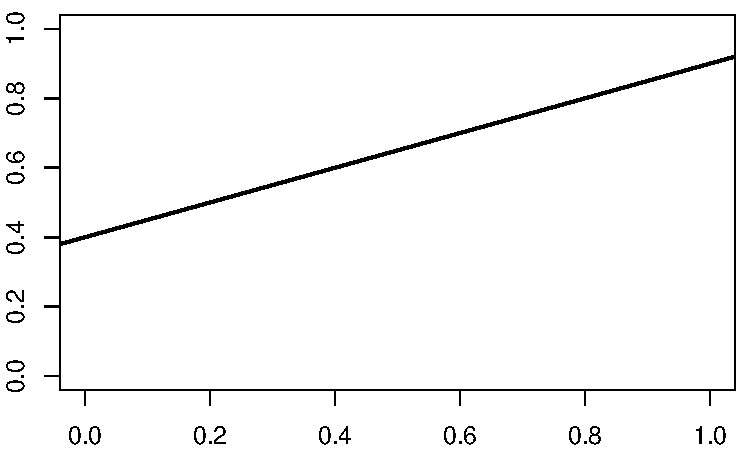
\includegraphics[width=0.5\textwidth]{./externalfig/linear_regression.pdf}
\end{center}
\end{frame}

%------------------------------------------------------------%

\begin{frame}[fragile]\frametitle{Linear models: Not only linear ...}
 \begin{block}{It is not that simple...}
 Be aware that with linear models only the parameterisation is linear.\\ The function can also be nonlinear.\\
 \(  y=ax -bx +cx^2  \) is a linear model\\
 \(  y=ax_1^2 +b \frac{x_2 + 1}{\sqrt{x_2-1}} +cx_3 *x_4^3  \) is a linear model\\
\end{block}
\begin{knitrout}
\definecolor{shadecolor}{rgb}{0.961, 0.961, 0.961}\color{fgcolor}\begin{kframe}
\begin{alltt}
\hlkwd{plot}\hlstd{(}\hlkwa{function}\hlstd{(}\hlkwc{x}\hlstd{)} \hlnum{1}\hlopt{*}\hlstd{x} \hlopt{-}\hlkwd{I}\hlstd{(}\hlnum{2}\hlopt{*}\hlstd{x)} \hlopt{+} \hlkwd{I}\hlstd{(}\hlnum{3}\hlopt{*}\hlstd{x}\hlopt{^}\hlnum{2}\hlstd{),} \hlkwc{xlim}\hlstd{=}\hlkwd{c}\hlstd{(}\hlopt{-}\hlnum{100}\hlstd{,} \hlnum{100}\hlstd{))}
\end{alltt}
\end{kframe}

{\centering \includegraphics[width=0.3\textwidth]{./fig/lmex1-1} 

}



\end{knitrout}
\end{frame}

%------------------------------------------------------------%

\begin{frame}[fragile]\frametitle{Linear Regression}
\begin{knitrout}
\definecolor{shadecolor}{rgb}{0.961, 0.961, 0.961}\color{fgcolor}\begin{kframe}
\begin{alltt}
\hlstd{reg.data} \hlkwb{<-} \hlkwd{read.table}\hlstd{(}\hlstr{"data/tannin.txt"}\hlstd{,}\hlkwc{header}\hlstd{=T)}
\hlkwd{attach}\hlstd{(reg.data);} \hlkwd{names}\hlstd{(reg.data)}
\end{alltt}
\begin{verbatim}
## [1] "growth" "tannin"
\end{verbatim}
\end{kframe}
\end{knitrout}
\end{frame}

%------------------------------------------------------------%

\begin{frame}[fragile]\frametitle{Linear Regression}
\begin{knitrout}
\definecolor{shadecolor}{rgb}{0.961, 0.961, 0.961}\color{fgcolor}\begin{kframe}
\begin{alltt}
\hlkwd{plot}\hlstd{(tannin, growth)}
\end{alltt}
\end{kframe}

{\centering \includegraphics[width=.8\textwidth]{./fig/mcregdataplot-1} 

}



\end{knitrout}
\end{frame}

%------------------------------------------------------------%

\begin{frame}[fragile]\frametitle{Assumptions and rules of Linear Regression}
\begin{itemize}
\item The variance in y is constant (i.e. does not change as y gets bigger).
\item The explanatory variable, x, is measured without error.
\item The difference between a measured value of y and the value predicted by the model for
the same value of x is called a residual.
\item Residuals are measured on the scale of y (i.e. parallel to the y axis).
\item The residuals are normally distributed
\end{itemize}
\begin{center}
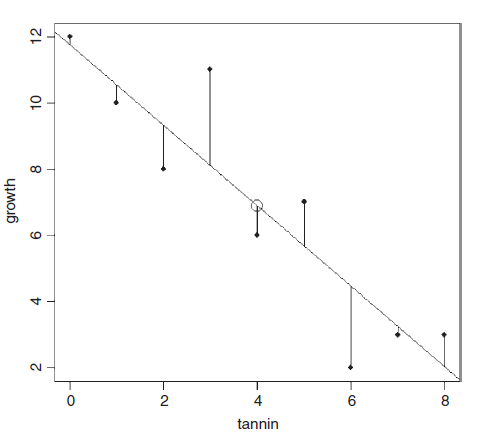
\includegraphics[width=0.4\textwidth]{./externalfig/tannin_residualsplot.png}
\end{center}
\end{frame}

%------------------------------------------------------------%

\begin{frame}[fragile]\frametitle{Fitting a linear model: specify a formula}
\begin{knitrout}
\definecolor{shadecolor}{rgb}{0.961, 0.961, 0.961}\color{fgcolor}\begin{kframe}
\begin{alltt}
\hlstd{mod} \hlkwb{<-} \hlkwd{lm}\hlstd{(growth}\hlopt{~}\hlstd{tannin)}
\hlcom{# visualise the model in a plot}
\hlkwd{plot}\hlstd{(growth}\hlopt{~}\hlstd{tannin)}
\hlcom{# easily done with abline}
\hlkwd{abline}\hlstd{(mod)}
\end{alltt}
\end{kframe}

{\centering \includegraphics[width=.4\textwidth]{./fig/lmxy-1} 

}



\end{knitrout}
\end{frame}

%------------------------------------------------------------%

\begin{frame}[fragile]\frametitle{Structure of an lm object I}
\begin{knitrout}\scriptsize
\definecolor{shadecolor}{rgb}{0.961, 0.961, 0.961}\color{fgcolor}\begin{kframe}
\begin{alltt}
\hlkwd{str}\hlstd{(mod,} \hlkwc{give.attr}\hlstd{=}\hlnum{FALSE}\hlstd{)}
\end{alltt}
\begin{verbatim}
## List of 12
##  $ coefficients : Named num [1:2] 11.76 -1.22
##  $ residuals    : Named num [1:9] 0.244 -0.539 -1.322 2.894 -0.889 ...
##  $ effects      : Named num [1:9] -20.67 -9.42 -1.32 2.83 -1.01 ...
##  $ rank         : int 2
##  $ fitted.values: Named num [1:9] 11.76 10.54 9.32 8.11 6.89 ...
##  $ assign       : int [1:2] 0 1
##  $ qr           :List of 5
##   ..$ qr   : num [1:9, 1:2] -3 0.333 0.333 0.333 0.333 ...
##   ..$ qraux: num [1:2] 1.33 1.26
##   ..$ pivot: int [1:2] 1 2
##   ..$ tol  : num 1e-07
##   ..$ rank : int 2
##  $ df.residual  : int 7
##  $ xlevels      : Named list()
##  $ call         : language lm(formula = growth ~ tannin)
##  $ terms        :Classes 'terms', 'formula' length 3 growth ~ tannin
##  $ model        :'data.frame':	9 obs. of  2 variables:
##   ..$ growth: int [1:9] 12 10 8 11 6 7 2 3 3
##   ..$ tannin: int [1:9] 0 1 2 3 4 5 6 7 8
\end{verbatim}
\end{kframe}
\end{knitrout}
\end{frame}


%------------------------------------------------------------%

\begin{frame}[fragile]\frametitle{Structure of an lm object II}
\begin{knitrout}\scriptsize
\definecolor{shadecolor}{rgb}{0.961, 0.961, 0.961}\color{fgcolor}\begin{kframe}
\begin{alltt}
\hlkwd{str}\hlstd{(mod[}\hlnum{1}\hlopt{:}\hlnum{6}\hlstd{])}
\end{alltt}
\begin{verbatim}
## List of 6
##  $ coefficients : Named num [1:2] 11.76 -1.22
##   ..- attr(*, "names")= chr [1:2] "(Intercept)" "tannin"
##  $ residuals    : Named num [1:9] 0.244 -0.539 -1.322 2.894 -0.889 ...
##   ..- attr(*, "names")= chr [1:9] "1" "2" "3" "4" ...
##  $ effects      : Named num [1:9] -20.67 -9.42 -1.32 2.83 -1.01 ...
##   ..- attr(*, "names")= chr [1:9] "(Intercept)" "tannin" "" "" ...
##  $ rank         : int 2
##  $ fitted.values: Named num [1:9] 11.76 10.54 9.32 8.11 6.89 ...
##   ..- attr(*, "names")= chr [1:9] "1" "2" "3" "4" ...
##  $ assign       : int [1:2] 0 1
\end{verbatim}
\end{kframe}
\end{knitrout}
\end{frame}

%------------------------------------------------------------%

\begin{frame}[fragile]\frametitle{Structure of an lm object III}
\begin{knitrout}\footnotesize
\definecolor{shadecolor}{rgb}{0.961, 0.961, 0.961}\color{fgcolor}\begin{kframe}
\begin{alltt}
\hlkwd{str}\hlstd{(mod[}\hlnum{7}\hlopt{:}\hlnum{10}\hlstd{])}
\end{alltt}
\begin{verbatim}
## List of 4
##  $ qr         :List of 5
##   ..$ qr   : num [1:9, 1:2] -3 0.333 0.333 0.333 0.333 ...
##   .. ..- attr(*, "dimnames")=List of 2
##   .. .. ..$ : chr [1:9] "1" "2" "3" "4" ...
##   .. .. ..$ : chr [1:2] "(Intercept)" "tannin"
##   .. ..- attr(*, "assign")= int [1:2] 0 1
##   ..$ qraux: num [1:2] 1.33 1.26
##   ..$ pivot: int [1:2] 1 2
##   ..$ tol  : num 1e-07
##   ..$ rank : int 2
##   ..- attr(*, "class")= chr "qr"
##  $ df.residual: int 7
##  $ xlevels    : Named list()
##  $ call       : language lm(formula = growth ~ tannin)
\end{verbatim}
\end{kframe}
\end{knitrout}
\end{frame}

%------------------------------------------------------------%

\begin{frame}[fragile]\frametitle{Structure of an lm object IV}
\begin{knitrout}\scriptsize
\definecolor{shadecolor}{rgb}{0.961, 0.961, 0.961}\color{fgcolor}\begin{kframe}
\begin{alltt}
\hlkwd{str}\hlstd{(mod[}\hlnum{11}\hlstd{])}
\end{alltt}
\begin{verbatim}
## List of 1
##  $ terms:Classes 'terms', 'formula' length 3 growth ~ tannin
##   .. ..- attr(*, "variables")= language list(growth, tannin)
##   .. ..- attr(*, "factors")= int [1:2, 1] 0 1
##   .. .. ..- attr(*, "dimnames")=List of 2
##   .. .. .. ..$ : chr [1:2] "growth" "tannin"
##   .. .. .. ..$ : chr "tannin"
##   .. ..- attr(*, "term.labels")= chr "tannin"
##   .. ..- attr(*, "order")= int 1
##   .. ..- attr(*, "intercept")= int 1
##   .. ..- attr(*, "response")= int 1
##   .. ..- attr(*, ".Environment")=<environment: R_GlobalEnv> 
##   .. ..- attr(*, "predvars")= language list(growth, tannin)
##   .. ..- attr(*, "dataClasses")= Named chr [1:2] "numeric" "numeric"
##   .. .. ..- attr(*, "names")= chr [1:2] "growth" "tannin"
\end{verbatim}
\end{kframe}
\end{knitrout}
\end{frame}

%------------------------------------------------------------%

\begin{frame}[fragile]\frametitle{Structure of an lm object V}
\begin{knitrout}\scriptsize
\definecolor{shadecolor}{rgb}{0.961, 0.961, 0.961}\color{fgcolor}\begin{kframe}
\begin{alltt}
\hlkwd{str}\hlstd{(mod[}\hlnum{12}\hlstd{])}
\end{alltt}
\begin{verbatim}
## List of 1
##  $ model:'data.frame':	9 obs. of  2 variables:
##   ..$ growth: int [1:9] 12 10 8 11 6 7 2 3 3
##   ..$ tannin: int [1:9] 0 1 2 3 4 5 6 7 8
##   ..- attr(*, "terms")=Classes 'terms', 'formula' length 3 growth ~ tannin
##   .. .. ..- attr(*, "variables")= language list(growth, tannin)
##   .. .. ..- attr(*, "factors")= int [1:2, 1] 0 1
##   .. .. .. ..- attr(*, "dimnames")=List of 2
##   .. .. .. .. ..$ : chr [1:2] "growth" "tannin"
##   .. .. .. .. ..$ : chr "tannin"
##   .. .. ..- attr(*, "term.labels")= chr "tannin"
##   .. .. ..- attr(*, "order")= int 1
##   .. .. ..- attr(*, "intercept")= int 1
##   .. .. ..- attr(*, "response")= int 1
##   .. .. ..- attr(*, ".Environment")=<environment: R_GlobalEnv> 
##   .. .. ..- attr(*, "predvars")= language list(growth, tannin)
##   .. .. ..- attr(*, "dataClasses")= Named chr [1:2] "numeric" "numeric"
##   .. .. .. ..- attr(*, "names")= chr [1:2] "growth" "tannin"
\end{verbatim}
\end{kframe}
\end{knitrout}
\end{frame}

%------------------------------------------------------------%

\begin{frame}[fragile]\frametitle{Standard output of an lm object}
\begin{knitrout}
\definecolor{shadecolor}{rgb}{0.961, 0.961, 0.961}\color{fgcolor}\begin{kframe}
\begin{alltt}
\hlstd{mod}
\end{alltt}
\begin{verbatim}
## 
## Call:
## lm(formula = growth ~ tannin)
## 
## Coefficients:
## (Intercept)       tannin  
##      11.756       -1.217
\end{verbatim}
\end{kframe}
\end{knitrout}
\end{frame}

%------------------------------------------------------------%

\begin{frame}[fragile]\frametitle{Your turn to practice regression ...}
\begin{exercise}{Explore the methods for lm} %ex12
\begin{enumerate}
\item read and plot the tannin data, fit and plot the linear model
\item Check out the following \rcode{lm} methods:
\begin{enumerate}
  \item \rcode{summary()}
  \item \rcode{fitted.values}
  \item \rcode{residuals}
  \item \rcode{anova}
  \item \rcode{plot} (click or press enter to continue)
\end{enumerate}
\item Bonus: plot the data, linear model, and add the line parameters into the plot
\end{enumerate}
\end{exercise}
\end{frame}

%------------------------------------------------------------%

\begin{frame}[fragile]\frametitle{Generic methods for linear model objects}
\begin{description}
\item[print]{standard output, returns formula and estimated coefficients}
\item[summary]{very infomative summary of the fit including statistics}
\item[coefficients]{shows the estimated values for the model coefficients}
\item[fitted.values]{returns the fitted values for the input dataset}
\item[update]{by specifying a formula, you can add or remove parameters from a model}
\item[residuals]{returns the residuals (unexplained variation)}
\item[deviance]{returns the sum of squares of the residuals (RSS)}
\item[anova]{returns an ANOVA table of the results}
\item[lm.influence]{identifies observations of high influence}
\item[predict]{use a model predict from a new dataset}
\item[plot]{diagnostic plot to analyse the quality of fit}
\end{description}
\end{frame}

%------------------------------------------------------------%

\begin{frame}[fragile]\frametitle{Solution for exercise \arabic{exercisecount}.1}
\begin{knitrout}\small
\definecolor{shadecolor}{rgb}{0.961, 0.961, 0.961}\color{fgcolor}\begin{kframe}
\begin{alltt}
\hlcom{# Data with plant growth and tannin level (a biomolecule)}
\hlstd{plants} \hlkwb{<-} \hlkwd{read.table}\hlstd{(}\hlstr{"data/tannin.txt"}\hlstd{,} \hlkwc{header}\hlstd{=}\hlnum{TRUE}\hlstd{)}
\hlkwd{str}\hlstd{(plants)}

\hlkwd{attach}\hlstd{(plant_data)} \hlcom{# Not good practice! confusing scoping!}
\hlcom{# attach creates objects of each column in the sub-environment:}
\hlkwd{ls}\hlstd{(}\hlkwc{pos}\hlstd{=}\hlnum{2}\hlstd{)}
\hlkwd{detach}\hlstd{(plant_data)}

\hlcom{# rather use:}
\hlkwd{plot}\hlstd{(growth} \hlopt{~} \hlstd{tannin,} \hlkwc{data}\hlstd{=plants)}

\hlcom{# linear model (lm) of growth depending on tannin:}
\hlstd{model} \hlkwb{<-} \hlkwd{lm}\hlstd{(growth} \hlopt{~} \hlstd{tannin,} \hlkwc{data}\hlstd{=plants)}
\hlstd{model}
\hlkwd{abline}\hlstd{(model)} \hlcom{# adds line to current plot}
\hlkwd{str}\hlstd{(model)}
\end{alltt}
\end{kframe}
\end{knitrout}
\end{frame}

%------------------------------------------------------------%

\begin{frame}[fragile]\frametitle{Solution for exercise \arabic{exercisecount}.2}
\begin{knitrout}
\definecolor{shadecolor}{rgb}{0.961, 0.961, 0.961}\color{fgcolor}\begin{kframe}
\begin{alltt}
\hlkwd{summary}\hlstd{(model)}
\hlcom{# Goodness of fit , coefficient of determination}
\hlkwd{summary}\hlstd{(model)}\hlopt{$}\hlstd{r.squared} \hlcom{# 0.8: pretty good, not perfect}

\hlcom{# what values are expected by the model:}
\hlkwd{fitted.values}\hlstd{(model)}
\hlkwd{points}\hlstd{(plants}\hlopt{$}\hlstd{tannin,} \hlkwd{fitted.values}\hlstd{(model),} \hlkwc{pch}\hlstd{=}\hlnum{16}\hlstd{,} \hlkwc{col}\hlstd{=}\hlnum{2}\hlstd{)}
\hlcom{# difference between each observation and modeled value:}
\hlkwd{residuals}\hlstd{(model)}

\hlcom{# Analysis of Variance (see the statistics books mentioned)}
\hlkwd{anova}\hlstd{(model)}
\hlcom{# many plots with statistical information are available:}
\hlkwd{plot}\hlstd{(model)}
\end{alltt}
\end{kframe}
\end{knitrout}
\end{frame}

%------------------------------------------------------------%

\begin{frame}[fragile]\frametitle{Solution for exercise \arabic{exercisecount}.3}
\begin{knitrout}
\definecolor{shadecolor}{rgb}{0.961, 0.961, 0.961}\color{fgcolor}\begin{kframe}
\begin{alltt}
\hlcom{# write Parameters of fit into the graph:}
\hlkwd{plot}\hlstd{(growth} \hlopt{~} \hlstd{tannin,} \hlkwc{data}\hlstd{=plants)}
\hlkwd{abline}\hlstd{(model,} \hlkwc{col}\hlstd{=}\hlnum{2}\hlstd{)}
\hlkwd{coef}\hlstd{(model)}
\hlcom{# y = m*x + b}
\hlstd{r} \hlkwb{<-} \hlkwd{round}\hlstd{(} \hlkwd{summary}\hlstd{(model)}\hlopt{$}\hlstd{r.squared ,}\hlkwc{digits}\hlstd{=}\hlnum{2}\hlstd{)}
\hlstd{m} \hlkwb{<-} \hlkwd{round}\hlstd{(} \hlkwd{coef}\hlstd{(model)[}\hlnum{2}\hlstd{] ,}\hlnum{2} \hlstd{)}
\hlstd{b} \hlkwb{<-} \hlkwd{round}\hlstd{(} \hlkwd{coef}\hlstd{(model)[}\hlnum{1}\hlstd{] ,}\hlnum{2} \hlstd{)}
\hlstd{Txt} \hlkwb{<-} \hlkwd{paste}\hlstd{(}\hlstr{"y ="}\hlstd{, m,} \hlstr{"* x +"}\hlstd{, b,} \hlstr{"\textbackslash{}nR^2 ="}\hlstd{, r)}
\hlstd{Txt}  \hlcom{#\textbackslash{}n for line break}
\hlkwd{text}\hlstd{(}\hlnum{5}\hlstd{,}\hlnum{10}\hlstd{, Txt,} \hlkwc{adj}\hlstd{=}\hlnum{0}\hlstd{,} \hlkwc{col}\hlstd{=}\hlnum{2}\hlstd{)}

\hlkwd{library}\hlstd{(berryFunctions)}
\hlkwd{linReg}\hlstd{(plants}\hlopt{$}\hlstd{tannin, plants}\hlopt{$}\hlstd{growth)} \hlcom{# for a quick lmplot}
\end{alltt}
\end{kframe}
\end{knitrout}
\end{frame}

%------------------------------------------------------------%

\begin{frame}[fragile]\frametitle{Summary of an lm object}
\begin{knitrout}\scriptsize
\definecolor{shadecolor}{rgb}{0.961, 0.961, 0.961}\color{fgcolor}\begin{kframe}
\begin{alltt}
\hlstd{oo} \hlkwb{<-} \hlkwd{options}\hlstd{(}\hlkwc{width}\hlstd{=}\hlnum{150}\hlstd{)}
\hlkwd{summary}\hlstd{(mod)}
\end{alltt}
\begin{verbatim}
## 
## Call:
## lm(formula = growth ~ tannin)
## 
## Residuals:
##     Min      1Q  Median      3Q     Max 
## -2.4556 -0.8889 -0.2389  0.9778  2.8944 
## 
## Coefficients:
##             Estimate Std. Error t value Pr(>|t|)    
## (Intercept)  11.7556     1.0408  11.295 9.54e-06 ***
## tannin       -1.2167     0.2186  -5.565 0.000846 ***
## ---
## Signif. codes:  0 '***' 0.001 '**' 0.01 '*' 0.05 '.' 0.1 ' ' 1
## 
## Residual standard error: 1.693 on 7 degrees of freedom
## Multiple R-squared:  0.8157,	Adjusted R-squared:  0.7893 
## F-statistic: 30.97 on 1 and 7 DF,  p-value: 0.0008461
\end{verbatim}
\end{kframe}
\end{knitrout}

\end{frame}

%------------------------------------------------------------%

\begin{frame}[fragile]\frametitle{Elements in the summary of a an lm object}
Here is an explanation of the terms in the summary \\[\baselineskip]
\small{
\begin{tabular}{ll}%{rlp{.5\textwidth}}
\texttt{Call:}              &  the way \rcode{lm} was called\\
\texttt{Residuals:}         &  descriptive statistics about the residuals\\
\texttt{Coefficients:}      &  statistical result for the estimated parameters\\
\texttt{- Estimate}         &  estimated value in the fit\\
\texttt{- Std Error}        &  standard error of the estimate \\
\texttt{- t value}          &  t value for the test statistic\\
\texttt{- Pr(\textgreater \textbar t\textbar)} & probability for the estimate to be 0\\
\texttt{Multiple R-squared} &  coefficient of determination (explained variation)\\
\texttt{Adjusted R-squared} &  adjusted for sample size and number of parameters\\
\texttt{degrees of freedom} &  sample size - number of predictors -1\\
% F-statistic & what is this?
\texttt{p-value}            &  significance of the regression \\
\end{tabular}
}
\end{frame}

%------------------------------------------------------------%

\begin{frame}[fragile]\frametitle{Coefficient of determination}
The coefficient of determination it a measure of how well a model fits to the data.\\
It shows you the part of variation within the data that is explained by the model.\\

\[R^2 \equiv 1 - \frac{SS_{\rm res}}{SS_{\rm tot}} \] 

with\\[\baselineskip]
\begin{tabular}{ll}
\(SS_{tot}=\sum_i (y_i-\bar{y})^2 \) & total sum of squares\\
\(SS_{reg}=\sum_i (f_i -\bar{y})^2 \)& regression (explained) sum of squares\\
\(SS_{res}=\sum_i (y_i - f_i)^2\ \) & sum of squares of residuals\\
\end{tabular} \\[\baselineskip]

Speak: \textit{The model explains XX \% of the variation.}
\end{frame}

%------------------------------------------------------------%

\begin{frame}[fragile]\frametitle{$R^2$ is not to be confused with Pearson r (correlation)}

The Pearson product-moment correlation coefficient r (also $\rho$):
\[ r_{xy} = \frac{
\sum_i^n(x_i - \bar{x})(y_i - \bar{y})
}{
\sqrt{\sum_i^n(x_i - \bar{x})^2 \sum_i^n(y_i - \bar{y})^2}}
\]

For the case of a linear model with a single variable $r=\sqrt{R^2}$
\end{frame}

%------------------------------------------------------------%

\begin{frame}[fragile]\frametitle{$R^2$ is not to be confused with Pearson r (correlation)}
For the case of a linear model with a single variable \[r=\sqrt{R^2}\]

\begin{knitrout}
\definecolor{shadecolor}{rgb}{0.961, 0.961, 0.961}\color{fgcolor}\begin{kframe}
\begin{alltt}
\hlcom{# Pearson r}
\hlkwd{cor}\hlstd{(tannin, growth)}
\end{alltt}
\begin{verbatim}
## [1] -0.9031408
\end{verbatim}
\begin{alltt}
\hlcom{# R-squared}
\hlkwd{sqrt}\hlstd{(}\hlkwd{summary}\hlstd{(mod)}\hlopt{$}\hlstd{r.squared)}
\end{alltt}
\begin{verbatim}
## [1] 0.9031408
\end{verbatim}
\end{kframe}
\end{knitrout}
\end{frame}

%------------------------------------------------------------%

%summary
%% measures of fit
%% significance: intercept
%% significance: slope

%------------------------------------------------------------%

\begin{frame}[fragile]\frametitle{Diagnostic plot of an lm object I}
As you saw before, for visualisation of the line you have to add it via \rcode{abline}, the \rcode{plot} function does a diagnostic plot:
%, tidy=T
\begin{knitrout}
\definecolor{shadecolor}{rgb}{0.961, 0.961, 0.961}\color{fgcolor}\begin{kframe}
\begin{alltt}
\hlcom{# allow 4 subplots with par(mfrow=c(2,2))}
\hlkwd{par}\hlstd{(}\hlkwc{mfrow}\hlstd{=}\hlkwd{c}\hlstd{(}\hlnum{2}\hlstd{,}\hlnum{2}\hlstd{));} \hlkwd{plot}\hlstd{(mod)}
\end{alltt}
\end{kframe}
\end{knitrout}
\end{frame}

%------------------------------------------------------------%

%, tidy=T


%------------------------------------------------------------%

\begin{frame}[fragile]\frametitle{Diagnostic plot of an lm object II}
\begin{center}
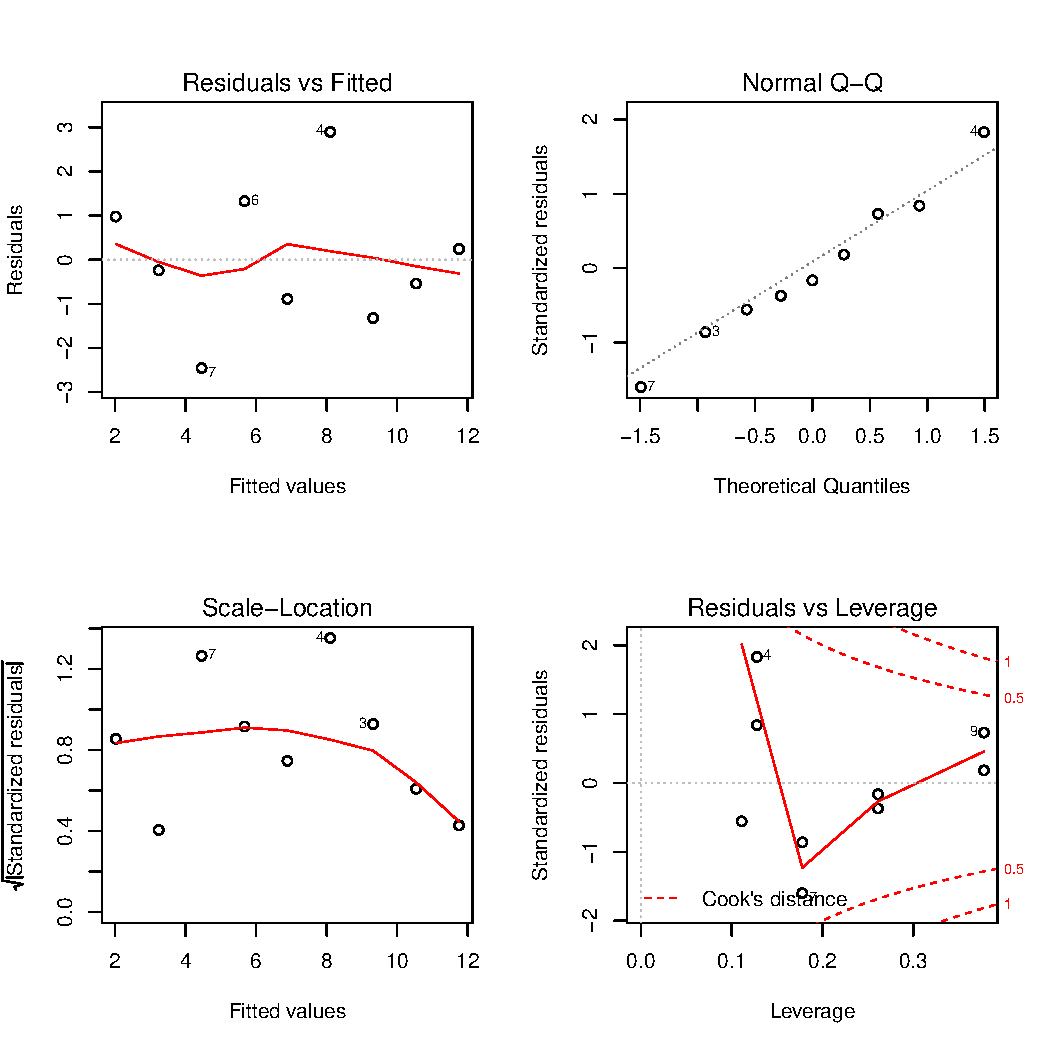
\includegraphics[width=.6\textwidth]{./externalfig/lmplot.pdf}
\end{center}
\end{frame}

%------------------------------------------------------------%

\begin{frame}[fragile]\frametitle{Measures of fit}
Corrected sums of squares and sums of products
\begin{description}
\item [y sums of squares] \( SSY=\sum y^2 - \frac{(\sum y)^2}{n}\)
\item [x sums of squares] \( SSX=\sum x^2 - \frac{(\sum x)^2}{n}\)
\item [$x*y$ sums of squares] \( SSXY=\sum xy - \frac{(\sum x)(\sum y)}{n}\)
\end{description}
\end{frame}

%------------------------------------------------------------%
%------------------------------------------------------------%
\subsection{Multivariate linear model}
%------------------------------------------------------------%
%------------------------------------------------------------%

\begin{frame}[fragile]\frametitle{Multivariate linear model I}
Before we actually look at multivariate models, let's examine another dataset:
\begin{knitrout}
\definecolor{shadecolor}{rgb}{0.961, 0.961, 0.961}\color{fgcolor}\begin{kframe}
\begin{alltt}
\hlkwd{class}\hlstd{(trees)}
\end{alltt}
\begin{verbatim}
## [1] "data.frame"
\end{verbatim}
\begin{alltt}
\hlkwd{head}\hlstd{(trees)}
\end{alltt}
\begin{verbatim}
##   Girth Height Volume
## 1   8.3     70   10.3
## 2   8.6     65   10.3
## 3   8.8     63   10.2
## 4  10.5     72   16.4
## 5  10.7     81   18.8
## 6  10.8     83   19.7
\end{verbatim}
\end{kframe}
\end{knitrout}
\end{frame}

%------------------------------------------------------------%

\begin{frame}[fragile]\frametitle{Multivariate linear model II}
\begin{knitrout}
\definecolor{shadecolor}{rgb}{0.961, 0.961, 0.961}\color{fgcolor}\begin{kframe}
\begin{alltt}
\hlcom{# Model with just Height:}
\hlstd{treemod_vh} \hlkwb{<-} \hlkwd{lm}\hlstd{(trees}\hlopt{$}\hlstd{Volume} \hlopt{~} \hlstd{trees}\hlopt{$}\hlstd{Height)}
\hlkwd{summary}\hlstd{(treemod_vh)}\hlopt{$}\hlstd{r.squared} \hlcom{# 0.3579026}
\end{alltt}
\begin{verbatim}
## [1] 0.3579026
\end{verbatim}
\begin{alltt}
\hlkwd{cor}\hlstd{(trees}\hlopt{$}\hlstd{Volume, trees}\hlopt{$}\hlstd{Height)}\hlopt{^}\hlnum{2} \hlcom{# 0.3579026 - the same}
\end{alltt}
\begin{verbatim}
## [1] 0.3579026
\end{verbatim}
\end{kframe}
\end{knitrout}
\onslide<2>
\begin{knitrout}
\definecolor{shadecolor}{rgb}{0.961, 0.961, 0.961}\color{fgcolor}\begin{kframe}
\begin{alltt}
\hlcom{# low correlation also visible:}
\hlkwd{plot}\hlstd{(trees}\hlopt{$}\hlstd{Volume} \hlopt{~} \hlstd{trees}\hlopt{$}\hlstd{Height)}
\hlkwd{abline}\hlstd{(treemod_vh,} \hlkwc{col}\hlstd{=}\hlnum{2}\hlstd{)}
\end{alltt}
\end{kframe}
\end{knitrout}
\end{frame}

%------------------------------------------------------------%

\begin{frame}[fragile]\frametitle{Multivariate linear model III}
\begin{knitrout}
\definecolor{shadecolor}{rgb}{0.961, 0.961, 0.961}\color{fgcolor}

{\centering \includegraphics[width=0.96\textwidth]{./fig/tree_heightc-1} 

}



\end{knitrout}
\end{frame}

%------------------------------------------------------------%

\begin{frame}[fragile]\frametitle{Multivariate linear model IV}
\begin{knitrout}
\definecolor{shadecolor}{rgb}{0.961, 0.961, 0.961}\color{fgcolor}\begin{kframe}
\begin{alltt}
\hlcom{# Just Height, but without intercept}
\hlcom{# (we know: Height=0 --> Vol=0)}
\hlstd{treemod_vh_noint} \hlkwb{<-} \hlkwd{update}\hlstd{(treemod_vh, .}\hlopt{~}\hlstd{.} \hlopt{-}\hlnum{1}\hlstd{)}
\hlstd{treemod_vh_noint}
\end{alltt}
\begin{verbatim}
## 
## Call:
## lm(formula = trees$Volume ~ trees$Height - 1)
## 
## Coefficients:
## trees$Height  
##       0.4047
\end{verbatim}
\end{kframe}
\end{knitrout}
\end{frame}

%------------------------------------------------------------%

\begin{frame}[fragile]\frametitle{Multivariate linear model V}
\begin{knitrout}
\definecolor{shadecolor}{rgb}{0.961, 0.961, 0.961}\color{fgcolor}\begin{kframe}
\begin{alltt}
\hlkwd{plot}\hlstd{(trees}\hlopt{$}\hlstd{Volume} \hlopt{~} \hlstd{trees}\hlopt{$}\hlstd{Height)}
\hlkwd{abline}\hlstd{(treemod_vh,} \hlkwc{col}\hlstd{=}\hlnum{2}\hlstd{)}
\hlkwd{abline}\hlstd{(treemod_vh_noint,} \hlkwc{col}\hlstd{=}\hlnum{4}\hlstd{)}
\end{alltt}
\end{kframe}

{\centering \includegraphics[width=0.85\textwidth]{./fig/tree_heighte-1} 

}



\end{knitrout}
\end{frame}

%------------------------------------------------------------%

\begin{frame}[fragile]\frametitle{Multivariate linear model VI}
\begin{knitrout}
\definecolor{shadecolor}{rgb}{0.961, 0.961, 0.961}\color{fgcolor}\begin{kframe}
\begin{alltt}
\hlcom{# just Girth:}
\hlkwd{cor}\hlstd{(trees}\hlopt{$}\hlstd{Volume, trees}\hlopt{$}\hlstd{Girth)}\hlopt{^}\hlnum{2} \hlcom{# 0.9353199 }
\end{alltt}
\begin{verbatim}
## [1] 0.9353199
\end{verbatim}
\begin{alltt}
\hlkwd{plot}\hlstd{(trees}\hlopt{$}\hlstd{Girth, trees}\hlopt{$}\hlstd{Volume,} \hlkwc{pch}\hlstd{=}\hlnum{16}\hlstd{)}
\end{alltt}
\end{kframe}

{\centering \includegraphics[width=0.7\textwidth]{./fig/tree_girth-1} 

}



\end{knitrout}
\end{frame}

%------------------------------------------------------------%

\begin{frame}[fragile]\frametitle{Multivariate linear model VII}
To include several predictors, use \rcode{+} in the lm formula.
\begin{knitrout}\small
\definecolor{shadecolor}{rgb}{0.961, 0.961, 0.961}\color{fgcolor}\begin{kframe}
\begin{alltt}
\hlcom{# Both:}
\hlstd{treemod_vhg} \hlkwb{<-} \hlkwd{lm}\hlstd{(Volume} \hlopt{~} \hlstd{Height} \hlopt{+} \hlstd{Girth,} \hlkwc{data}\hlstd{=trees)}
\hlstd{treemod_vhg}
\end{alltt}
\begin{verbatim}
## 
## Call:
## lm(formula = Volume ~ Height + Girth, data = trees)
## 
## Coefficients:
## (Intercept)       Height        Girth  
##    -57.9877       0.3393       4.7082
\end{verbatim}
\end{kframe}
\end{knitrout}
\end{frame}

%------------------------------------------------------------%

\begin{frame}[fragile]\frametitle{Multivariate linear model VIII}
\begin{knitrout}
\definecolor{shadecolor}{rgb}{0.961, 0.961, 0.961}\color{fgcolor}\begin{kframe}
\begin{alltt}
\hlcom{# Both:}
\hlkwd{summary}\hlstd{(treemod_vhg)}\hlopt{$}\hlstd{r.squared}
\end{alltt}
\begin{verbatim}
## [1] 0.94795
\end{verbatim}
\end{kframe}
\end{knitrout}
Volume prediction from Height not good, from Girth pretty OK.\\
Prediction from both variables not much better than just Girth.
\onslide<2>
\begin{knitrout}
\definecolor{shadecolor}{rgb}{0.961, 0.961, 0.961}\color{fgcolor}\begin{kframe}
\begin{alltt}
\hlcom{# Both:}
\hlkwd{summary}\hlstd{(treemod_vhg)}\hlopt{$}\hlstd{r.squared}
\end{alltt}
\begin{verbatim}
## [1] 0.94795
\end{verbatim}
\end{kframe}
\end{knitrout}
\end{frame}

%------------------------------------------------------------%

\begin{frame}[fragile]\frametitle{Your turn  ...}
\begin{exercise}{multivariate model} %ex13
We measured another tree. The girth is 15 inches and height 70 feet.
\begin{enumerate}
\item Estimate the wood volume by using the \rcode{coef}\texttt{ficients} of the linear model that just uses height as predictor.
\item Estimate it with another regression just using girth.
\item Use the multivariate model to estimate wood volume.
\item What are possibilities and dangers of linear regression models?
\item Bonus: Give uncertainty ranges for the model parameters
\item Bonus: Give uncertainty ranges for the estimates
\end{enumerate}
\end{exercise}
\end{frame}

%------------------------------------------------------------%

\begin{frame}[fragile]\frametitle{Solution for exercise \arabic{exercisecount}.2-3}
\begin{knitrout}
\definecolor{shadecolor}{rgb}{0.961, 0.961, 0.961}\color{fgcolor}\begin{kframe}
\begin{alltt}
\hlkwd{coef}\hlstd{(} \hlkwd{lm}\hlstd{(trees}\hlopt{$}\hlstd{Volume} \hlopt{~} \hlstd{trees}\hlopt{$}\hlstd{Girth) )}
\end{alltt}
\begin{verbatim}
## (Intercept) trees$Girth 
##  -36.943459    5.065856
\end{verbatim}
\begin{alltt}
\hlkwd{coef}\hlstd{(treemod_vhg)}
\end{alltt}
\begin{verbatim}
## (Intercept)      Height       Girth 
## -57.9876589   0.3392512   4.7081605
\end{verbatim}
\end{kframe}
\end{knitrout}
\onslide<2>
\begin{knitrout}
\definecolor{shadecolor}{rgb}{0.961, 0.961, 0.961}\color{fgcolor}\begin{kframe}
\begin{alltt}
\hlnum{0.339} \hlopt{*} \hlnum{70}  \hlopt{+}  \hlnum{4.708} \hlopt{*} \hlnum{15}  \hlopt{-}  \hlnum{57.988} \hlcom{# 36.36 }
\hlnum{5.066} \hlopt{*} \hlnum{15}  \hlopt{-}  \hlnum{36.943} \hlcom{# 39.05        cubic feet}
\end{alltt}
\end{kframe}
\end{knitrout}
There is some variation naturally, so we don't know which result is "correct".
\end{frame}

%------------------------------------------------------------%

\begin{frame}[fragile]\frametitle{Solution for exercise \arabic{exercisecount}.5-6}
\begin{knitrout}
\definecolor{shadecolor}{rgb}{0.961, 0.961, 0.961}\color{fgcolor}\begin{kframe}
\begin{alltt}
\hlcom{# prediction confidence interval:}
\hlkwd{predict}\hlstd{(treemod_vhg,} \hlkwc{newdata}\hlstd{=}
    \hlkwd{data.frame}\hlstd{(}\hlkwc{Girth}\hlstd{=}\hlnum{15}\hlstd{,} \hlkwc{Height}\hlstd{=}\hlnum{70}\hlstd{),} \hlkwc{interval}\hlstd{=}\hlstr{"conf"}\hlstd{)}
\end{alltt}
\begin{verbatim}
##        fit      lwr      upr
## 1 36.38234 33.72289 39.04178
\end{verbatim}
\begin{alltt}
\hlcom{# parameter uncertainty:}
\hlkwd{confint}\hlstd{(treemod_vhg)}
\end{alltt}
\begin{verbatim}
##                    2.5 %      97.5 %
## (Intercept) -75.68226247 -40.2930554
## Height        0.07264863   0.6058538
## Girth         4.16683899   5.2494820
\end{verbatim}
\end{kframe}
\end{knitrout}
\end{frame}

%------------------------------------------------------------%

\begin{frame}[fragile]\frametitle{Solution for exercise \arabic{exercisecount}.5 II}
\begin{knitrout}
\definecolor{shadecolor}{rgb}{0.961, 0.961, 0.961}\color{fgcolor}\begin{kframe}
\begin{alltt}
\hlkwd{library}\hlstd{(}\hlstr{"berryFunctions"}\hlstd{)} \hlcom{# for addAlpha}
\hlkwd{plot}\hlstd{(Volume}\hlopt{~}\hlstd{Girth,} \hlkwc{data}\hlstd{=trees,} \hlkwc{las}\hlstd{=}\hlnum{1}\hlstd{)}
\hlstd{mod} \hlkwb{<-} \hlkwd{lm}\hlstd{(Volume}\hlopt{~}\hlstd{Girth,} \hlkwc{data}\hlstd{=trees)}
\hlstd{x} \hlkwb{<-} \hlnum{7}\hlopt{:}\hlnum{22}
\hlstd{mod_p} \hlkwb{<-} \hlkwd{predict}\hlstd{(mod,} \hlkwc{newdata}\hlstd{=}\hlkwd{data.frame}\hlstd{(}\hlkwc{Girth}\hlstd{=x),}
                 \hlkwc{interval}\hlstd{=}\hlstr{"conf"}\hlstd{)}
\hlkwd{polygon}\hlstd{(}\hlkwc{x}\hlstd{=}\hlkwd{c}\hlstd{(x,} \hlkwd{rev}\hlstd{(x)),}
        \hlkwc{y}\hlstd{=}\hlkwd{c}\hlstd{(mod_p[,}\hlnum{2}\hlstd{],} \hlkwd{rev}\hlstd{(mod_p[,}\hlnum{3}\hlstd{])),} \hlkwc{col}\hlstd{=}\hlkwd{addAlpha}\hlstd{(}\hlnum{8}\hlstd{))}
\hlkwd{abline}\hlstd{(mod,} \hlkwc{col}\hlstd{=}\hlnum{2}\hlstd{,} \hlkwc{lwd}\hlstd{=}\hlnum{2}\hlstd{)}
\end{alltt}
\end{kframe}
\end{knitrout}
\end{frame}

%------------------------------------------------------------%

\begin{frame}[fragile]\frametitle{Solution for exercise \arabic{exercisecount}.5 III}
\begin{knitrout}
\definecolor{shadecolor}{rgb}{0.961, 0.961, 0.961}\color{fgcolor}

{\centering \includegraphics[width=1\textwidth]{./fig/ex12sole-1} 

}



\end{knitrout}
\end{frame}

%------------------------------------------------------------%
%------------------------------------------------------------%
\subsection{Multiple linear model (ANCOVA)}
%------------------------------------------------------------%
%------------------------------------------------------------%

\begin{frame}[fragile]\frametitle{Multiple linear models (MLM)}
\begin{description}
\item [y sums of squares] \( SSY=\sum y^2 - \frac{(\sum y)^2}{n}\)
\item [x sums of squares] \( SSX=\sum x^2 - \frac{(\sum x)^2}{n}\)
\item [$x*y$ sums of squares] \( SSXY=\sum xy - \frac{(\sum x)(\sum y)}{n}\)
\end{description}
\end{frame}

%------------------------------------------------------------%

% use of glm: some more comfortable features

% %------------------------------------------------------------%

\begin{frame}[fragile]\frametitle{MLM example: The ANalysis of COVAriance}
In this example we will look at a special case of the multiple linear model: The ANalysis of COVAriance (ANCOVA).\\[\baselineskip]
You will improve your knowledge about:
\begin{itemize}
\item how to specify a formula
\item how to combine continous and nominally scaled predictors
\item introduction of interaction
\item an alternative plotting environment
\end{itemize}
\end{frame}

%------------------------------------------------------------%

\begin{frame}[fragile]\frametitle{MLM example with the iris dataset}
Overview of the correlation structure
\begin{knitrout}
\definecolor{shadecolor}{rgb}{0.961, 0.961, 0.961}\color{fgcolor}\begin{kframe}
\begin{alltt}
\hlkwd{cor}\hlstd{(iris[,}\hlnum{1}\hlopt{:}\hlnum{4}\hlstd{])}
\end{alltt}
\begin{verbatim}
##              Sepal.Length Sepal.Width
## Sepal.Length    1.0000000  -0.1175698
## Sepal.Width    -0.1175698   1.0000000
## Petal.Length    0.8717538  -0.4284401
## Petal.Width     0.8179411  -0.3661259
##              Petal.Length Petal.Width
## Sepal.Length    0.8717538   0.8179411
## Sepal.Width    -0.4284401  -0.3661259
## Petal.Length    1.0000000   0.9628654
## Petal.Width     0.9628654   1.0000000
\end{verbatim}
\end{kframe}
\end{knitrout}
We will attempt to set up a model for Sepal.Width
\end{frame}

%------------------------------------------------------------%

\begin{frame}[fragile]\frametitle{MLM example with the iris dataset}
Get to know the data: specify a plotting formula



\begin{knitrout}\small
\definecolor{shadecolor}{rgb}{0.961, 0.961, 0.961}\color{fgcolor}\begin{kframe}
\begin{alltt}
\hlkwd{par}\hlstd{(}\hlkwc{mfrow}\hlstd{=}\hlkwd{c}\hlstd{(}\hlnum{2}\hlstd{,}\hlnum{2}\hlstd{),} \hlkwc{mar}\hlstd{=}\hlkwd{c}\hlstd{(}\hlnum{4}\hlstd{,}\hlnum{4}\hlstd{,}\hlnum{1}\hlstd{,}\hlnum{1}\hlstd{))}
\hlkwd{plot}\hlstd{(Sepal.Width} \hlopt{~} \hlstd{Sepal.Length} \hlopt{+} \hlstd{Petal.Length} \hlopt{+}
       \hlstd{Petal.Width} \hlopt{+} \hlstd{Species,} \hlkwc{col}\hlstd{=Species)}
\end{alltt}
\end{kframe}

{\centering \includegraphics[width=0.8\linewidth]{./fig/irisexpplot-1} 

}



\end{knitrout}

\end{frame}

%------------------------------------------------------------%

\begin{frame}[fragile]\frametitle{MLM example with the iris dataset}
For you to take a closer look at: A classical Scatterplot
\begin{knitrout}
\definecolor{shadecolor}{rgb}{0.961, 0.961, 0.961}\color{fgcolor}\begin{kframe}
\begin{alltt}
\hlkwd{library}\hlstd{(lattice)}
\hlkwd{splom}\hlstd{(iris)}
\end{alltt}
\end{kframe}

{\centering \includegraphics[width=.8\textwidth]{./fig/irissplom-1} 

}



\end{knitrout}
\end{frame}

%------------------------------------------------------------%


% ANCOVA for Sepal.Length ~ Sepal.Length

%------------------------------------------------------------%

\begin{frame}[fragile]\frametitle{MLM example with the iris dataset}
\begin{knitrout}
\definecolor{shadecolor}{rgb}{0.961, 0.961, 0.961}\color{fgcolor}\begin{kframe}
\begin{alltt}
\hlcom{# lattice library xyplot for groups highlighting}
\hlkwd{xyplot}\hlstd{(}\hlkwc{data}\hlstd{=iris, Sepal.Width} \hlopt{~} \hlstd{Sepal.Length,}
       \hlkwc{groups}\hlstd{=Species,} \hlkwc{auto.key}\hlstd{=T)}
\end{alltt}
\end{kframe}

{\centering \includegraphics[width=.8\textwidth]{./fig/irissepwidthplot-1} 

}



\end{knitrout}
\end{frame}

%------------------------------------------------------------%

\begin{frame}[fragile]\frametitle{MLM example with the iris dataset I}
Fitting a linear model using \rcode{glm} since it has some comfortable arguments.\\[\baselineskip]
Both species \textit{Iris versicolor} and  \textit{Iris virginica} have a slope significantly different from  \textit{Iris setosa}, as can be seen in the next slide:
\end{frame}

%------------------------------------------------------------%

\begin{frame}[fragile]\frametitle{MLM example with the iris dataset II}

\begin{knitrout}\tiny
\definecolor{shadecolor}{rgb}{0.961, 0.961, 0.961}\color{fgcolor}\begin{kframe}
\begin{alltt}
\hlkwd{summary}\hlstd{(}\hlkwd{glm}\hlstd{(Sepal.Width} \hlopt{~} \hlstd{Sepal.Length} \hlopt{*} \hlstd{Species,} \hlkwc{data}\hlstd{=iris))}
\end{alltt}
\begin{verbatim}
## 
## Call:
## glm(formula = Sepal.Width ~ Sepal.Length * Species, data = iris)
## 
## Deviance Residuals: 
##      Min        1Q    Median        3Q       Max  
## -0.72394  -0.16327  -0.00289   0.16457   0.60954  
## 
## Coefficients:
##                                Estimate Std. Error t value Pr(>|t|)    
## (Intercept)                     -0.5694     0.5539  -1.028 0.305622    
## Sepal.Length                     0.7985     0.1104   7.235 2.55e-11 ***
## Speciesversicolor                1.4416     0.7130   2.022 0.045056 *  
## Speciesvirginica                 2.0157     0.6861   2.938 0.003848 ** 
## Sepal.Length:Speciesversicolor  -0.4788     0.1337  -3.582 0.000465 ***
## Sepal.Length:Speciesvirginica   -0.5666     0.1262  -4.490 1.45e-05 ***
## ---
## Signif. codes:  0 '***' 0.001 '**' 0.01 '*' 0.05 '.' 0.1 ' ' 1
## 
## (Dispersion parameter for gaussian family taken to be 0.07416645)
## 
##     Null deviance: 28.307  on 149  degrees of freedom
## Residual deviance: 10.680  on 144  degrees of freedom
## AIC: 43.342
## 
## Number of Fisher Scoring iterations: 2
\end{verbatim}
\end{kframe}
\end{knitrout}

\end{frame}

%------------------------------------------------------------%

\begin{frame}[fragile]\frametitle{MLM example with the iris dataset III}
We remove \textit{Iris setosa} from the plot by introducing a \rcode{subset}.
\begin{knitrout}
\definecolor{shadecolor}{rgb}{0.961, 0.961, 0.961}\color{fgcolor}\begin{kframe}
\begin{alltt}
\hlkwd{xyplot}\hlstd{(}\hlkwc{data}\hlstd{=iris, Sepal.Width} \hlopt{~} \hlstd{Sepal.Length,}
  \hlkwc{groups}\hlstd{=Species,} \hlkwc{auto.key}\hlstd{=T,} \hlkwc{subset}\hlstd{=Species}\hlopt{!=}\hlstr{"setosa"}\hlstd{)}
\end{alltt}
\end{kframe}

{\centering \includegraphics[width=.8\textwidth]{./fig/irisswsubsplot-1} 

}



\end{knitrout}
\end{frame}

%------------------------------------------------------------%

\begin{frame}[fragile]\frametitle{MLM example with the iris dataset IV}
%In the same way we remove \textit{Iris setosa} from the model with a \rcode{subset}.
% , tidy.opts=list(keep.blank.line=FALSE, width.cutoff=60)


\begin{knitrout}\tiny
\definecolor{shadecolor}{rgb}{0.961, 0.961, 0.961}\color{fgcolor}\begin{kframe}
\begin{alltt}
 \hlkwd{summary}\hlstd{(}\hlkwd{glm}\hlstd{(Sepal.Width} \hlopt{~} \hlstd{Sepal.Length} \hlopt{*} \hlstd{Species,} \hlkwc{data}\hlstd{=iris,} \hlkwc{subset}\hlstd{=Species}\hlopt{!=}\hlstr{"setosa"}\hlstd{))}
\end{alltt}
\begin{verbatim}
## 
## Call:
## glm(formula = Sepal.Width ~ Sepal.Length * Species, data = iris, 
##     subset = Species != "setosa")
## 
## Deviance Residuals: 
##      Min        1Q    Median        3Q       Max  
## -0.65441  -0.13553  -0.00134   0.16638   0.60954  
## 
## Coefficients:
##                               Estimate Std. Error t value Pr(>|t|)    
## (Intercept)                    0.87215    0.46155   1.890   0.0618 .  
## Sepal.Length                   0.31972    0.07747   4.127 7.83e-05 ***
## Speciesvirginica               0.57416    0.62146   0.924   0.3579    
## Sepal.Length:Speciesvirginica -0.08783    0.09978  -0.880   0.3809    
## ---
## Signif. codes:  0 '***' 0.001 '**' 0.01 '*' 0.05 '.' 0.1 ' ' 1
## 
## (Dispersion parameter for gaussian family taken to be 0.07834681)
## 
##     Null deviance: 10.9616  on 99  degrees of freedom
## Residual deviance:  7.5213  on 96  degrees of freedom
## AIC: 35.045
## 
## Number of Fisher Scoring iterations: 2
\end{verbatim}
\end{kframe}
\end{knitrout}

\end{frame}

%------------------------------------------------------------%

\begin{frame}[fragile]\frametitle{MLM example with the iris dataset}
Neither the slope nor the intercept of \textit{Iris versiculor} and  \textit{Iris virginica} are significantly different. \\
\medskip
For the model we can group them by creating a new factor.
\begin{knitrout}
\definecolor{shadecolor}{rgb}{0.961, 0.961, 0.961}\color{fgcolor}\begin{kframe}
\begin{alltt}
\hlstd{iris}\hlopt{$}\hlstd{SETOSA} \hlkwb{<-} \hlstd{iris}\hlopt{$}\hlstd{Species}
\hlkwd{levels}\hlstd{(iris}\hlopt{$}\hlstd{SETOSA)}\hlkwb{=}\hlkwd{c}\hlstd{(}\hlstr{"setosa"}\hlstd{,} \hlstr{"other"}\hlstd{,} \hlstr{"other"}\hlstd{)}
\hlkwd{summary}\hlstd{(iris}\hlopt{$}\hlstd{SETOSA)}
\end{alltt}
\begin{verbatim}
## setosa  other 
##     50    100
\end{verbatim}
\end{kframe}
\end{knitrout}
Now we can go back to the full data set and create a model with the new factor: (next slide)

\end{frame}

%------------------------------------------------------------%

\begin{frame}[fragile]\frametitle{MLM example with the iris dataset}
% xyplot(data=iris, Sepal.Width ~ Sepal.Length, groups=SETOSA, auto.key=T)

\begin{knitrout}\tiny
\definecolor{shadecolor}{rgb}{0.961, 0.961, 0.961}\color{fgcolor}\begin{kframe}
\begin{alltt}
\hlkwd{summary}\hlstd{(sw.lm} \hlkwb{<-} \hlkwd{glm}\hlstd{(Sepal.Width} \hlopt{~} \hlstd{Sepal.Length} \hlopt{*} \hlstd{SETOSA,} \hlkwc{data}\hlstd{=iris))}
\end{alltt}
\begin{verbatim}
## 
## Call:
## glm(formula = Sepal.Width ~ Sepal.Length * SETOSA, data = iris)
## 
## Deviance Residuals: 
##      Min        1Q    Median        3Q       Max  
## -0.72394  -0.17751   0.00646   0.17304   0.60085  
## 
## Coefficients:
##                          Estimate Std. Error t value Pr(>|t|)    
## (Intercept)               -0.5694     0.5521  -1.031  0.30402    
## Sepal.Length               0.7985     0.1100   7.259 2.14e-11 ***
## SETOSAother                1.7003     0.6099   2.788  0.00601 ** 
## Sepal.Length:SETOSAother  -0.5205     0.1175  -4.431 1.83e-05 ***
## ---
## Signif. codes:  0 '***' 0.001 '**' 0.01 '*' 0.05 '.' 0.1 ' ' 1
## 
## (Dispersion parameter for gaussian family taken to be 0.0736832)
## 
##     Null deviance: 28.307  on 149  degrees of freedom
## Residual deviance: 10.758  on 146  degrees of freedom
## AIC: 40.43
## 
## Number of Fisher Scoring iterations: 2
\end{verbatim}
\end{kframe}
\end{knitrout}

\end{frame}

%------------------------------------------------------------%

\begin{frame}[fragile]\frametitle{MLM example with the iris dataset}
Plotting using lattice is powerful but takes some time getting used to it.
\begin{knitrout}\small
\definecolor{shadecolor}{rgb}{0.961, 0.961, 0.961}\color{fgcolor}\begin{kframe}
\begin{alltt}
\hlkwd{xyplot}\hlstd{(}\hlkwc{data}\hlstd{=iris, Sepal.Width} \hlopt{~} \hlstd{Sepal.Length,} \hlkwc{groups}\hlstd{=SETOSA,}
       \hlkwc{auto.key}\hlstd{=T,} \hlkwc{col}\hlstd{=}\hlkwd{c}\hlstd{(}\hlstr{"darkslateblue"}\hlstd{,} \hlstr{"tomato2"}\hlstd{),}
        \hlkwc{panel}\hlstd{=}\hlkwa{function}\hlstd{(}\hlkwc{x}\hlstd{,}\hlkwc{y}\hlstd{,}\hlkwc{...}\hlstd{)}
          \hlstd{\{}\hlkwd{panel.xyplot}\hlstd{(x,y,...)}
          \hlkwd{panel.abline}\hlstd{(}\hlkwd{coef}\hlstd{(sw.lm)[}\hlnum{1}\hlopt{:}\hlnum{2}\hlstd{],}
                       \hlkwc{col}\hlstd{=}\hlstr{"darkslateblue"}\hlstd{,} \hlkwc{lwd}\hlstd{=}\hlnum{2}\hlstd{)}
          \hlkwd{panel.abline}\hlstd{(}\hlkwd{coef}\hlstd{(sw.lm)[}\hlnum{3}\hlopt{:}\hlnum{4}\hlstd{]} \hlopt{+} \hlkwd{coef}\hlstd{(sw.lm)[}\hlnum{1}\hlopt{:}\hlnum{2}\hlstd{],}
                       \hlkwc{col}\hlstd{=}\hlstr{"tomato2"}\hlstd{,} \hlkwc{lwd}\hlstd{=}\hlnum{2}\hlstd{)\})}
\end{alltt}
\end{kframe}
\end{knitrout}
\end{frame}

%------------------------------------------------------------%



%------------------------------------------------------------%

\begin{frame}[fragile]\frametitle{MLM example with the iris dataset}
\begin{center}
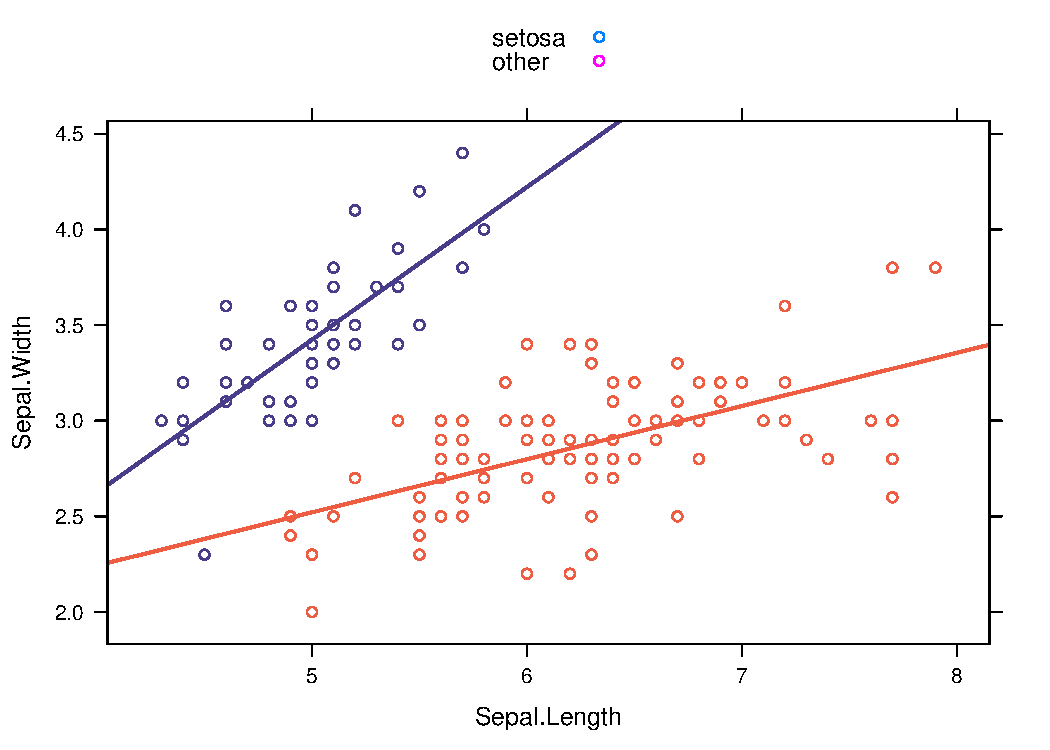
\includegraphics[width=0.8\textwidth]{./externalfig/sepalwidth_ancovaplot.pdf}
\end{center}
\end{frame}

%------------------------------------------------------------%

\begin{frame}[fragile]\frametitle{Specifying a formula}
\begin{block}{Formula operators used for \rcode{lm}, \rcode{anova}, \rcode{lattice}, ...}
\begin{tabular}{ll}
$\sim$ & ...\\
1 & intercept\\
: & interaction term\\
* & factor crossing, a*b is same as a+b+a:b\\
\^{} & crossing to the specified degree\\
- & removes specified term when updating a model\\
%\%in\% & left term nested within the right: \texttt{a + b \%in\% a} is same as \texttt{a + a:b} \\
\rcode{I}() & operators inside parenthesis are used literally\\
. & used for \rcode{update} of a formula, refers to the existing parameters\\
\textbar & conditional on\\
\end{tabular}
\end{block}
\end{frame}

%------------------------------------------------------------%

\begin{frame}[fragile]\frametitle{Your turn ...}
\begin{exercise}{Fit a model for \texttt{Petal.Width} and \texttt{Sepal.Width}} %ex14
\begin{enumerate}
\item Find out if there is a relation between Petal.Width and Petal.Length. Is it significant? What is the coefficient of determination? Interpret the graph.
\item Is there a relationship between Sepal.Width and Petal.Width? Is there a difference between species? Create a model based on the relationships you find. Only use significant variables.
\end{enumerate}
\end{exercise}
\end{frame}

%------------------------------------------------------------%

% \begin{frame}[fragile]\frametitle{Solution for exercise \arabic{exercisecount}.1}
% <<ex13sola, eval=FALSE>>=
% # ToDo
% @
% \end{frame}

%------------------------------------------------------------%

% % Bad boxes!
% % exercise with Petal.Width ~ Petal.Length
% <<irispetwidlm>>=
% attach(iris)
% plot(Petal.Width ~ Petal.Length) # grouping of points
% # fit a model anyways
% abline(pw.lm <- lm(Petal.Width ~ Petal.Length))
% summary(pw.lm)
% par(mfrow=c(2,2), mar=c(4,4,3,0.5)); plot(pw.lm)
% detach(iris)
% @
% 
% % exercise with Sepal.Width ~ Petal.Width
% <<irissepwidex>>=
% xyplot(data=iris, Sepal.Width ~ Petal.Width, groups=Species, auto.key=T)
% summary(model0 <- glm(Sepal.Width ~ Petal.Width * Species, data=iris))
% summary(glm(Sepal.Width ~ Petal.Width, subset=Species=="setosa", data=iris))
% xyplot(data=iris, Sepal.Width ~ Petal.Width, groups=Species, subset=Species!="setosa", col=c("darkslateblue", "tomato2"))
% summary(swlm1 <- glm(Sepal.Width ~ Petal.Width * Species, data=iris, subset=Species!="setosa"))
% # There is a significant difference in the intercept, but not in the slope, lets remove the interaction, then
% swlm2 <- update(swlm1, ~ . - Petal.Width:Species)
% summary(swlm2)
% xyplot(data=iris, Sepal.Width ~ Petal.Width, groups=Species, subset=Species!="setosa", col=c("darkslateblue", "tomato2"), panel=function(x,y,...){panel.xyplot(x,y,...)
%                                panel.abline(coef(swlm2)[1:2], col="tomato2", lwd=2)
%                                panel.abline(coef(swlm2)[1:2] + c(coef(swlm2)[3],0), col="darkslateblue", lwd=2)})
% # conclusions: versicolor and virginica differ in the intercept, but not in their slope
% @
% 
% <<irisancovaplot>>=
% plot(data=iris, Sepal.Width ~ Sepal.Length, groups=Species, auto.key=T)
% @
% 
% 9:00 - 10:30: linear models, regression (spearman), ANOVA, histogram, ks.test
% 11:00 - 12:30: exercise

% linear regression
% SSE, SSR, SSY, SSX, SSXY
% formula definition
% return values of lm
% multiple linear model
% sepal oder DEWFORA
% scatterplot
% update
% overfitting
% correlation matrix
% aicfit
% exercise with relating snow cover to elevation -> after spatial lesson is done

%\href{http://www.statmethods.net/stats/regression.html}{statmethods.net/stats/regression}

%------------------------------------------------------------%

% \begin{frame}[fragile]\frametitle{Ideas for more} 
% \begin{itemize}
% \item Find a correct solution for a model of tree volume as a function of tree height and girth
% \item PERSIANN rainfall data from binary files
% \end{itemize}
% \end{frame}

%------------------------------------------------------------%
%------------------------------------------------------------%
\section{Time series handling and analysis}
%------------------------------------------------------------%
%------------------------------------------------------------%

%------------------------------------------------------------%
%------------------------------------------------------------%
\subsection{Background on time series}
%------------------------------------------------------------%
%------------------------------------------------------------%

\begin{frame}\frametitle{Authorship note} 
% make note to first slide clickable.
This section (time series) was originally written by Matthias Seibert (see note on the first slide). I heavily borrowed from his slides and wish to thankfully acknowledge his work!

\begin{knitrout}
\definecolor{shadecolor}{rgb}{0.961, 0.961, 0.961}\color{fgcolor}\begin{kframe}
\begin{alltt}
\hlkwd{library}\hlstd{(xts)}
\end{alltt}
\end{kframe}
\end{knitrout}
\end{frame}

%------------------------------------------------------------%

\begin{frame}\frametitle{Types of time series}
\begin{itemize}
\item regularly spaced time series
% , cache=T, dev='pdf', out.width=".9\\linewidth">>=
\begin{knitrout}
\definecolor{shadecolor}{rgb}{0.961, 0.961, 0.961}\color{fgcolor}

{\centering \includegraphics[width=.8\textwidth]{./fig/regularts-1} 

}



\end{knitrout}
\item irregularly spaced time series
\begin{knitrout}
\definecolor{shadecolor}{rgb}{0.961, 0.961, 0.961}\color{fgcolor}

{\centering \includegraphics[width=.8\textwidth]{./fig/irregularts-1} 

}



\end{knitrout}
\end{itemize}
\end{frame}

%------------------------------------------------------------%

\begin{frame}\frametitle{Complexity of time objects}
\begin{itemize}
\item time zones \medskip\\
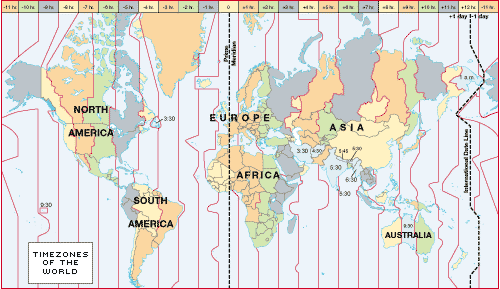
\includegraphics[width=0.4\textwidth]{externalfig/timezones.png}
\item various formats
\begin{itemize}
  \item \texttt{11.12.2013 12:00}
  \item \texttt{2013-12-11 12:00:00 GMT}
  \item \texttt{12/11/2013 12:00 am}
\end{itemize}
\end{itemize}
\end{frame}

%------------------------------------------------------------%

\begin{frame}\frametitle{The benefit of using time series classes}
\begin{itemize}
\item adjusted plotting
\item make the computer "understand" time: rules for addition, subtraction
\item deal with leap years
\item aggregation
\item reformatting and conversion: for example julian days to date
\item advanced time series analysis \footnote{usage of time classes are not a precondition in general}
\end{itemize}
\end{frame}

%------------------------------------------------------------%

\begin{frame}\frametitle{General information and packages}
  There's a lot of information on the \href{http://cran.r-project.org/web/views/TimeSeries.html}{R Task view on time series}.

  \vspace{2em}

	This workshop will mainly deal with the libraries: 
	\begin{itemize}
		\item \href{http://cran.r-project.org/web/packages/zoo/index.html}{\texttt{zoo}} 
		\item \href{http://cran.r-project.org/web/packages/xts/index.html}{\texttt{xts}}
	\end{itemize}
	and methods associated with those classes.

	\vspace{2em}

	We (Mathias and Berry) consider "time" as a very complicated thing, which
	means, we have some knowledge gaps about that topic, too.

\end{frame}

%------------------------------------------------------------%

\begin{frame}\frametitle{We will have to deal with two aspects in the following section}
  learn how to deal with:
  \begin{description}
  \item[time itself]{handling time objects}
  \item[time series]{handling time series objects}
  \end{description}
\end{frame}

%------------------------------------------------------------%
%------------------------------------------------------------%
\subsection{Importing time series information}
%------------------------------------------------------------%
%------------------------------------------------------------%

\begin{frame}\frametitle{Where we want to get in this lecture ...}
At the end of the part of this lecture we want to create a time series of monthly temperature of a station in Tien Shan
\begin{figure}[h]
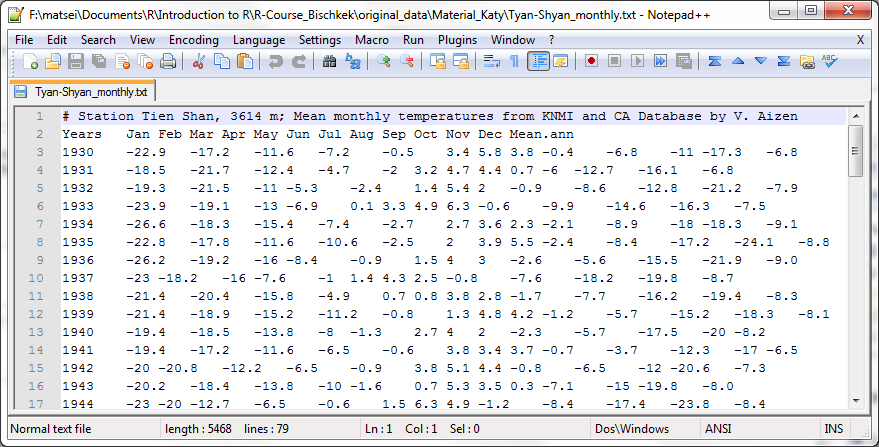
\includegraphics[width=0.9\textwidth]{./externalfig/SS_Tyan-Shyan_monthly_txt.png}
\caption{Format of the file \texttt{data/Tyan-Shyan\_monthly.txt}, monthly and annual temp}
\end{figure}
% \begin{itemize}
% \end{itemize}
\end{frame}

%------------------------------------------------------------%



%------------------------------------------------------------%

\begin{frame}\frametitle{Reading time series data from textfiles}
  \begin{itemize}
 \item simple example: 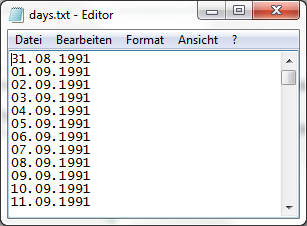
\includegraphics[scale=0.4]{./externalfig/SS_days.png}
 \item Dates in a standard format
 \end{itemize}
\end{frame}

%------------------------------------------------------------%

\begin{frame}\frametitle{Main function \rcode{strptime}}
\begin{itemize}
\item from character to time (POSIXct)
\begin{knitrout}
\definecolor{shadecolor}{rgb}{0.961, 0.961, 0.961}\color{fgcolor}\begin{kframe}
\begin{alltt}
\hlkwd{strptime}\hlstd{(x, format,} \hlkwc{tz} \hlstd{=} \hlstr{""}\hlstd{)}
\end{alltt}
\end{kframe}
\end{knitrout}
\item from time to character
\begin{knitrout}
\definecolor{shadecolor}{rgb}{0.961, 0.961, 0.961}\color{fgcolor}\begin{kframe}
\begin{alltt}
\hlkwd{format}\hlstd{(x,} \hlkwc{format} \hlstd{=} \hlstr{""}\hlstd{,} \hlkwc{tz} \hlstd{=} \hlstr{""}\hlstd{,} \hlkwc{usetz} \hlstd{=} \hlnum{FALSE}\hlstd{, ...)}
\end{alltt}
\end{kframe}
\end{knitrout}
\end{itemize}
\end{frame}

%------------------------------------------------------------%

\begin{frame}\frametitle{Specifiying the input format of the time input}
% charcters in the format string not interpretable as conversions specificators
\begin{block}{POSIX standard for text-dat/time conversion specifications}
\begin{tabular}{ll}
\texttt{\%A (\%a)} & Full (abbreviated) weekday name \footnote{in the current locale}\\
\texttt{\%B (\%b)} & Full (abbreviated) month name \footnote{in the current locale}\\
\texttt{\%d} & Day of the month as decimal number (01-31)\\
\texttt{\%m} & Month as decimal number (01-12)\\
\texttt{\%Y (\%y)} & Year with (without) century (00-99)\\
\texttt{\%H} & Hours as decimal number (00-23)\\
\texttt{\%M} & Minute as decimal number (00-59)\\
\texttt{\%S} & Second as decimal number (00-61)\footnote{accepts up to two leap seconds}\\
\texttt{\%j} & Day of year as decimal number (001-366)\\
\end{tabular}
\end{block}
see \rcode{help(strptime)} for details and more 
\end{frame}

%------------------------------------------------------------%

\begin{frame}[fragile]\frametitle{Importing \texttt{days.txt}}
\begin{knitrout}
\definecolor{shadecolor}{rgb}{0.961, 0.961, 0.961}\color{fgcolor}\begin{kframe}
\begin{alltt}
\hlstd{days.o} \hlkwb{<-} \hlkwd{scan}\hlstd{(}\hlkwc{file}\hlstd{=}\hlstr{"data/days.txt"}\hlstd{,} \hlkwc{what}\hlstd{=}\hlstr{"character"}\hlstd{)}
\hlstd{days1} \hlkwb{<-} \hlkwd{strptime}\hlstd{(}\hlkwc{x}\hlstd{=days.o,} \hlkwc{format}\hlstd{=}\hlstr{"%d.%m.%Y"}\hlstd{)}
\hlkwd{head}\hlstd{(days1)}
\end{alltt}
\begin{verbatim}
## [1] "1991-08-31 CEST" "1991-09-01 CEST"
## [3] "1991-09-02 CEST" "1991-09-03 CEST"
## [5] "1991-09-04 CEST" "1991-09-05 CEST"
\end{verbatim}
\begin{alltt}
\hlstd{days2} \hlkwb{<-} \hlkwd{as.Date}\hlstd{(}\hlkwc{x}\hlstd{=days.o,} \hlkwc{format}\hlstd{=}\hlstr{"%d.%m.%Y"}\hlstd{)}
\hlkwd{head}\hlstd{(days2)}
\end{alltt}
\begin{verbatim}
## [1] "1991-08-31" "1991-09-01"
## [3] "1991-09-02" "1991-09-03"
## [5] "1991-09-04" "1991-09-05"
\end{verbatim}
\end{kframe}
\end{knitrout}
\end{frame}

%------------------------------------------------------------%

\begin{frame}\frametitle{Your turn ...}
  \begin{exercise}{Import times from a text file} %ex15
  \label{ex:importtime}
Practice the specification of the \rcode{format} in \rcode{strptime} or \rcode{as.Date} by adapting it to the formats in the following files, which you will find in the \texttt{data} directory:
\begin{enumerate}
    \item \texttt{juliandays.txt}
    \item \texttt{daystimes.txt}
    \item \texttt{daystext.txt}
    \item \texttt{daysmonthtext.txt}
    \end{enumerate}
  \end{exercise}
\end{frame}

%------------------------------------------------------------%

\begin{frame}[fragile]\frametitle{Solution for exercise \arabic{exercisecount}}
\begin{knitrout}\tiny
\definecolor{shadecolor}{rgb}{0.961, 0.961, 0.961}\color{fgcolor}\begin{kframe}
\begin{alltt}
\hlstd{file1} \hlkwb{<-} \hlkwd{strptime}\hlstd{(}\hlkwc{format}\hlstd{=}\hlstr{"%Y-%j"}\hlstd{,} \hlkwc{x}\hlstd{=}\hlkwd{scan}\hlstd{(}\hlstr{"data/juliandays.txt"}\hlstd{,} \hlkwc{what}\hlstd{=}\hlstr{"character"}\hlstd{))}
\hlstd{file2} \hlkwb{<-} \hlkwd{strptime}\hlstd{(}\hlkwc{format}\hlstd{=}\hlstr{"%Y-%d-%m_(%H:%M)"}\hlstd{,} \hlkwc{x}\hlstd{=}\hlkwd{scan}\hlstd{(}\hlstr{"data/daystimes.txt"}\hlstd{,} \hlkwc{what}\hlstd{=}\hlstr{"character"}\hlstd{))}
\hlstd{file3} \hlkwb{<-} \hlkwd{strptime}\hlstd{(}\hlkwc{format}\hlstd{=}\hlstr{"Year:%Y_Month:%m_Day:%d"}\hlstd{,} \hlkwc{x}\hlstd{=}\hlkwd{scan}\hlstd{(}\hlstr{"data/daystext.txt"}\hlstd{,} \hlkwc{what}\hlstd{=}\hlstr{"character"}\hlstd{))}
\hlstd{file4} \hlkwb{<-} \hlkwd{strptime}\hlstd{(}\hlkwc{format}\hlstd{=}\hlstr{"%d_day_of_%B_%Y"}\hlstd{,} \hlkwc{x}\hlstd{=}\hlkwd{scan}\hlstd{(}\hlstr{"data/daysmonthtext.txt"}\hlstd{,} \hlkwc{what}\hlstd{=}\hlstr{"character"}\hlstd{))}
\end{alltt}
\end{kframe}
\end{knitrout}
\end{frame}

%------------------------------------------------------------%

\begin{frame}[fragile]\frametitle{Solution for exercise \arabic{exercisecount}.1}
\begin{knitrout}
\definecolor{shadecolor}{rgb}{0.961, 0.961, 0.961}\color{fgcolor}\begin{kframe}
\begin{alltt}
\hlstd{time1} \hlkwb{<-} \hlkwd{scan}\hlstd{(}\hlstr{"data/juliandays.txt"}\hlstd{,} \hlkwc{what}\hlstd{=}\hlstr{"character"}\hlstd{)}
\hlkwd{str}\hlstd{(time1)}
\end{alltt}
\begin{verbatim}
##  chr [1:6876] "1991-243" ...
\end{verbatim}
\begin{alltt}
\hlstd{time1} \hlkwb{<-} \hlkwd{strptime}\hlstd{(}\hlkwc{x}\hlstd{=time1,} \hlkwc{format}\hlstd{=}\hlstr{"%Y-%j"}\hlstd{)}
\hlkwd{str}\hlstd{(time1)}
\end{alltt}
\begin{verbatim}
##  POSIXlt[1:6876], format: "1991-08-31" "1991-09-01" ...
\end{verbatim}
\end{kframe}
\end{knitrout}
\end{frame}

%------------------------------------------------------------%

\begin{frame}[fragile]\frametitle{Solution for exercise \arabic{exercisecount}.I}
\begin{knitrout}
\definecolor{shadecolor}{rgb}{0.961, 0.961, 0.961}\color{fgcolor}\begin{kframe}
\begin{alltt}
\hlstd{time2} \hlkwb{<-} \hlkwd{scan}\hlstd{(}\hlstr{"data/daystimes.txt"}\hlstd{,} \hlkwc{what}\hlstd{=}\hlstr{"character"}\hlstd{)}
\hlkwd{str}\hlstd{(time2)}
\end{alltt}
\begin{verbatim}
##  chr [1:6876] "1991-31-08_(12:00)" ...
\end{verbatim}
\begin{alltt}
\hlstd{time2} \hlkwb{<-} \hlkwd{strptime}\hlstd{(}\hlkwc{x}\hlstd{=time2,} \hlkwc{format}\hlstd{=}\hlstr{"%Y-%d-%m_(%H:%M)"}\hlstd{)}
\hlkwd{str}\hlstd{(time2)}
\end{alltt}
\begin{verbatim}
##  POSIXlt[1:6876], format: "1991-08-31 12:00:00" ...
\end{verbatim}
\end{kframe}
\end{knitrout}
\end{frame}

%------------------------------------------------------------%

\begin{frame}[fragile]\frametitle{Solution for exercise \arabic{exercisecount}.II}
\begin{knitrout}
\definecolor{shadecolor}{rgb}{0.961, 0.961, 0.961}\color{fgcolor}\begin{kframe}
\begin{alltt}
\hlstd{t3} \hlkwb{<-} \hlkwd{scan}\hlstd{(}\hlstr{"data/daystext.txt"}\hlstd{,} \hlkwc{what}\hlstd{=}\hlstr{"character"}\hlstd{)}
\hlkwd{str}\hlstd{(t3)}
\end{alltt}
\begin{verbatim}
##  chr [1:6876] "Year:1991_Month:08_Day:31" ...
\end{verbatim}
\begin{alltt}
\hlstd{t3} \hlkwb{<-} \hlkwd{strptime}\hlstd{(}\hlkwc{x}\hlstd{=t3,} \hlkwc{format}\hlstd{=}\hlstr{"Year:%Y_Month:%m_Day:%d"}\hlstd{)}
\hlkwd{str}\hlstd{(t3)}
\end{alltt}
\begin{verbatim}
##  POSIXlt[1:6876], format: "1991-08-31" "1991-09-01" ...
\end{verbatim}
\end{kframe}
\end{knitrout}
\end{frame}

%------------------------------------------------------------%

\begin{frame}[fragile]\frametitle{Solution for exercise \arabic{exercisecount}.V}
\begin{knitrout}
\definecolor{shadecolor}{rgb}{0.961, 0.961, 0.961}\color{fgcolor}\begin{kframe}
\begin{alltt}
\hlstd{time4} \hlkwb{<-} \hlkwd{scan}\hlstd{(}\hlstr{"data/daysmonthtext.txt"}\hlstd{,} \hlkwc{what}\hlstd{=}\hlstr{"character"}\hlstd{)}
\hlkwd{str}\hlstd{(time4)}
\end{alltt}
\begin{verbatim}
##  chr [1:6876] "31_day_of_August_1991" ...
\end{verbatim}
\begin{alltt}
\hlstd{time4} \hlkwb{<-} \hlkwd{strptime}\hlstd{(}\hlkwc{x}\hlstd{=time4,} \hlkwc{format}\hlstd{=}\hlstr{"%d_day_of_%B_%Y"}\hlstd{)}
\hlkwd{str}\hlstd{(time4)}
\end{alltt}
\begin{verbatim}
##  POSIXlt[1:6876], format: "1991-08-31" "1991-09-01" ...
\end{verbatim}
\end{kframe}
\end{knitrout}
\end{frame}

%------------------------------------------------------------%

\begin{frame}[fragile]\frametitle{Difference of \texttt{strptime} and \texttt{as.Date} I}
\begin{knitrout}
\definecolor{shadecolor}{rgb}{0.961, 0.961, 0.961}\color{fgcolor}\begin{kframe}
\begin{alltt}
\hlcom{# Remember:}
\hlstd{days1} \hlkwb{<-} \hlkwd{strptime}\hlstd{(}\hlkwc{x}\hlstd{=days.o,} \hlkwc{format}\hlstd{=}\hlstr{"%d.%m.%Y"}\hlstd{)}
\hlstd{days2} \hlkwb{<-}  \hlkwd{as.Date}\hlstd{(}\hlkwc{x}\hlstd{=days.o,} \hlkwc{format}\hlstd{=}\hlstr{"%d.%m.%Y"}\hlstd{)}

\hlcom{# the strptime object}
\hlkwd{str}\hlstd{(days1)}
\end{alltt}
\begin{verbatim}
##  POSIXlt[1:6876], format: "1991-08-31" "1991-09-01" ...
\end{verbatim}
\begin{alltt}
\hlcom{# the as.Date object}
\hlkwd{str}\hlstd{(days2)}
\end{alltt}
\begin{verbatim}
##  Date[1:6876], format: "1991-08-31" "1991-09-01" ...
\end{verbatim}
\end{kframe}
\end{knitrout}
\end{frame}

%------------------------------------------------------------%

\begin{frame}[fragile]\frametitle{Difference of \texttt{strptime} and \texttt{as.Date} II}
\begin{knitrout}
\definecolor{shadecolor}{rgb}{0.961, 0.961, 0.961}\color{fgcolor}\begin{kframe}
\begin{alltt}
\hlcom{# the strptime object}
\hlkwd{head}\hlstd{(}\hlkwd{as.numeric}\hlstd{(days1))}
\end{alltt}
\begin{verbatim}
## [1] 683589600 683676000 683762400
## [4] 683848800 683935200 684021600
\end{verbatim}
\begin{alltt}
\hlcom{# the as.Date object}
\hlkwd{head}\hlstd{(}\hlkwd{as.numeric}\hlstd{(days2))}
\end{alltt}
\begin{verbatim}
## [1] 7912 7913 7914 7915 7916 7917
\end{verbatim}
\end{kframe}
\end{knitrout}
\begin{itemize}
\item Internally, the two objects are saved differently
\end{itemize}
\end{frame}

%------------------------------------------------------------%

\begin{frame}[fragile]\frametitle{Date and time objects}
There are several classes that deal specifically with time and date objects
\begin{description}
\item[POSIX] class with Portable Operating System Interface standard (POSIXct, POSIXlt) is the do-it-all option with support of date and time, timezones and daylight/standard times, saved as seconds since  January 1, 1970 GMT (POSIXct)\\
%\item[chron] dates and times also represented as days since January 1, 1970 only represents year and month, hence only suitable for monthly data\\
\item[Date] class for date only, infrastructure for regular and irregular time series, represents number of days since 1970-01-01, with negative values for earlier dates\\
\item[zoo::yearmon] only represents year and month, hence only suitable for monthly data, internally it saves data as the year + 0 for January and  year + 1/12 for February and so on\\
%datetime
% classes
\end{description}
\end{frame}

%------------------------------------------------------------%

\begin{frame}[fragile]\frametitle{Let us understand a little bit more about R ...}
Wikipedia: 
\begin{quote}
Object-oriented programming (OOP) is a programming paradigm that represents concepts as "objects" that have data fields (attributes that describe the object) and associated procedures known as methods.
\end{quote}
\begin{block}{Classes in R}
\begin{description}
\item[classes] in R are definitions of object structures.
\item[methods] are functions that are adapted to the class
\item[inheritance] means that one class can extend on another class while keeping its structure and associated methods. 
\end{description}
\end{block}
% example: str summary applicable to many objects
\end{frame}

%------------------------------------------------------------%

\begin{frame}[fragile]\frametitle{Class inquiry}
Retrieving class information 
% , tidy=T
\begin{knitrout}
\definecolor{shadecolor}{rgb}{0.961, 0.961, 0.961}\color{fgcolor}\begin{kframe}
\begin{alltt}
\hlkwd{class}\hlstd{(days1)}
\end{alltt}
\begin{verbatim}
## [1] "POSIXlt" "POSIXt"
\end{verbatim}
\begin{alltt}
\hlkwd{str}\hlstd{(days1)}
\end{alltt}
\begin{verbatim}
##  POSIXlt[1:6876], format: "1991-08-31" "1991-09-01" ...
\end{verbatim}
\end{kframe}
\end{knitrout}
\end{frame}

%------------------------------------------------------------%

\begin{frame}[fragile]\frametitle{Class inquiry}
Retrieving information about a class 
% , tidy=T
\begin{knitrout}
\definecolor{shadecolor}{rgb}{0.961, 0.961, 0.961}\color{fgcolor}\begin{kframe}
\begin{alltt}
\hlkwd{getClass}\hlstd{(}\hlstr{"POSIXct"}\hlstd{)}
\end{alltt}
\begin{verbatim}
## Virtual Class "POSIXct" [package "methods"]
## 
## Slots:
##                 
## Name:   .S3Class
## Class: character
## 
## Extends: 
## Class "POSIXt", directly
## Class "oldClass", by class "POSIXt", distance 2
\end{verbatim}
\end{kframe}
\end{knitrout}
\end{frame}

%------------------------------------------------------------%

\begin{frame}\frametitle{Importing a time series from a text file}
Back to the example of the monthly temperature of Tien Shan
\begin{figure}[h]
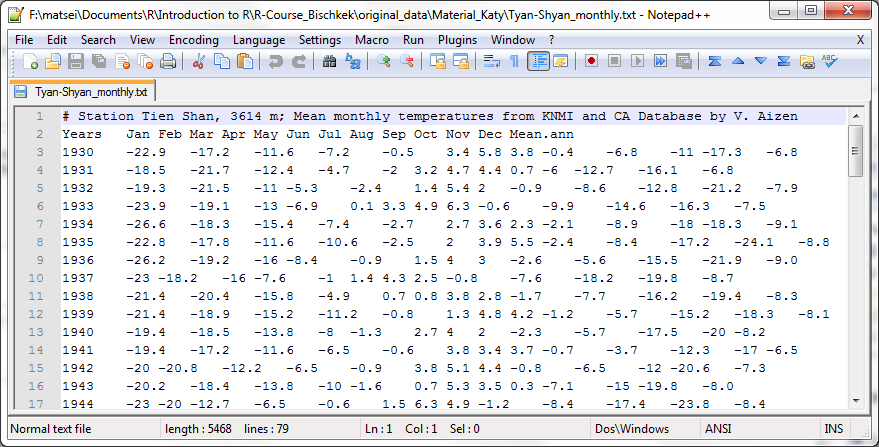
\includegraphics[width=0.5\textwidth]{./externalfig/SS_Tyan-Shyan_monthly_txt.png}
\end{figure}
 \begin{itemize}
\item tab delimited text
\item monthly and annual means in one file
\item one header in 2nd line
\item only years are supplied
 \end{itemize}
\end{frame}

%------------------------------------------------------------%

\begin{frame}[fragile]\frametitle{Importing a time series from a text file}
first, import the text file

\begin{knitrout}
\definecolor{shadecolor}{rgb}{0.961, 0.961, 0.961}\color{fgcolor}\begin{kframe}
\begin{alltt}
\hlstd{TienShan.dat} \hlkwb{<-} \hlkwd{read.table}\hlstd{(}\hlstr{"data/Tyan-Shyan_monthly.txt"}\hlstd{,}
                           \hlkwc{header} \hlstd{= T,}\hlkwc{sep}\hlstd{=}\hlstr{"\textbackslash{}t"}\hlstd{,} \hlkwc{skip}\hlstd{=}\hlnum{1}\hlstd{)}
\end{alltt}
\end{kframe}
\end{knitrout}
\begin{knitrout}\tiny
\definecolor{shadecolor}{rgb}{0.961, 0.961, 0.961}\color{fgcolor}\begin{kframe}
\begin{alltt}
\hlkwd{head}\hlstd{(TienShan.dat)} \hlcom{# display the data frame}
\end{alltt}
\begin{verbatim}
##   Years   Jan   Feb   Mar   Apr  May Jun Jul Aug  Sep  Oct   Nov   Dec Mean.ann
## 1  1930 -22.9 -17.2 -11.6  -7.2 -0.5 3.4 5.8 3.8 -0.4 -6.8 -11.0 -17.3     -6.8
## 2  1931 -18.5 -21.7 -12.4  -4.7 -2.0 3.2 4.7 4.4  0.7 -6.0 -12.7 -16.1     -6.8
## 3  1932 -19.3 -21.5 -11.0  -5.3 -2.4 1.4 5.4 2.0 -0.9 -8.6 -12.8 -21.2     -7.9
## 4  1933 -23.9 -19.1 -13.0  -6.9  0.1 3.3 4.9 6.3 -0.6 -9.9 -14.6 -16.3     -7.5
## 5  1934 -26.6 -18.3 -15.4  -7.4 -2.7 2.7 3.6 2.3 -2.1 -8.9 -18.0 -18.3     -9.1
## 6  1935 -22.8 -17.8 -11.6 -10.6 -2.5 2.0 3.9 5.5 -2.4 -8.4 -17.2 -24.1     -8.8
\end{verbatim}
\end{kframe}
\end{knitrout}

\end{frame}

%------------------------------------------------------------%

\begin{frame}[fragile]\frametitle{Importing a time series from a text file}
from the \rcode{data.frame} we can extract the monthly and/or the annual values:
\begin{knitrout}
\definecolor{shadecolor}{rgb}{0.961, 0.961, 0.961}\color{fgcolor}\begin{kframe}
\begin{alltt}
\hlcom{# create xts object of the annual temperatures}
\hlcom{# create time object from supplied dates}
\hlstd{annt} \hlkwb{<-} \hlkwd{as.yearmon}\hlstd{(}\hlkwd{paste}\hlstd{(}\hlstr{"Dec"}\hlstd{, TienShan.dat[,}\hlnum{1}\hlstd{]))}
\hlstd{tann.tiens} \hlkwb{<-} \hlkwd{xts}\hlstd{(TienShan.dat[,}\hlnum{14}\hlstd{],} \hlkwc{order.by}\hlstd{=annt)}
\hlkwd{colnames}\hlstd{(tann.tiens)} \hlkwb{<-} \hlstr{"TIENSHAN"}
\hlkwd{head}\hlstd{(tann.tiens,}\hlnum{3}\hlstd{)}
\end{alltt}
\begin{verbatim}
##          TIENSHAN
## Dec 1930     -6.8
## Dec 1931     -6.8
## Dec 1932     -7.9
\end{verbatim}
\end{kframe}
\end{knitrout}
\end{frame}

%------------------------------------------------------------%

\begin{frame}[fragile]\frametitle{Importing a time series from a text file}
from the \rcode{data.frame} we can extract the monthly and/or the annual values:
\begin{knitrout}
\definecolor{shadecolor}{rgb}{0.961, 0.961, 0.961}\color{fgcolor}\begin{kframe}
\begin{alltt}
\hlcom{# create xts object of the monthly temperatures}
\hlstd{timerange} \hlkwb{<-} \hlkwd{as.Date}\hlstd{(}\hlkwd{paste}\hlstd{(}\hlkwd{range}\hlstd{(TienShan.dat[,}\hlnum{1}\hlstd{]),}
                           \hlkwd{c}\hlstd{(}\hlstr{"-01-01"}\hlstd{,} \hlstr{"-12-01"}\hlstd{),} \hlkwc{sep}\hlstd{=}\hlstr{""}\hlstd{))}
\hlcom{# create time:}
\hlstd{mont} \hlkwb{<-} \hlkwd{seq}\hlstd{(}\hlkwd{first}\hlstd{(timerange),} \hlkwd{last}\hlstd{(timerange),} \hlkwc{by}\hlstd{=}\hlstr{"month"}\hlstd{)}
\hlstd{mont} \hlkwb{<-} \hlkwd{as.yearmon}\hlstd{(mont)}
\hlstd{tmon.tiens} \hlkwb{<-} \hlkwd{xts}\hlstd{(}\hlkwd{c}\hlstd{(}\hlkwd{t}\hlstd{(TienShan.dat[,}\hlnum{2}\hlopt{:}\hlnum{13}\hlstd{])),} \hlkwc{order.by}\hlstd{=mont)}
\end{alltt}
\end{kframe}
\end{knitrout}
\end{frame}

%------------------------------------------------------------%
%------------------------------------------------------------%
\subsection{Manipulation of time series}
%------------------------------------------------------------%
%------------------------------------------------------------%

\begin{frame}[fragile]\frametitle{Methods for date and time objects I}
Make functions from package "zoo" available:
\begin{knitrout}
\definecolor{shadecolor}{rgb}{0.961, 0.961, 0.961}\color{fgcolor}\begin{kframe}
\begin{alltt}
\hlkwd{library}\hlstd{(zoo)}
\hlstd{now} \hlkwb{<-} \hlkwd{Sys.time}\hlstd{()}
\hlstd{now}
\end{alltt}
\begin{verbatim}
## [1] "2015-10-15 15:47:10 CEST"
\end{verbatim}
\end{kframe}
\end{knitrout}
\end{frame}

%------------------------------------------------------------%

\begin{frame}[fragile]\frametitle{Methods for date and time objects II}
Conversion from one class to another follows the \rcode{as.*} syntax
\begin{knitrout}
\definecolor{shadecolor}{rgb}{0.961, 0.961, 0.961}\color{fgcolor}\begin{kframe}
\begin{alltt}
\hlkwd{class}\hlstd{(now)}
\end{alltt}
\begin{verbatim}
## [1] "POSIXct" "POSIXt"
\end{verbatim}
\begin{alltt}
\hlkwd{as.Date}\hlstd{(now)}
\end{alltt}
\begin{verbatim}
## [1] "2015-10-15"
\end{verbatim}
\begin{alltt}
\hlkwd{as.yearmon}\hlstd{(now)}
\end{alltt}
\begin{verbatim}
## [1] "Oct 2015"
\end{verbatim}
\end{kframe}
\end{knitrout}
\end{frame}

%------------------------------------------------------------%

\begin{frame}[fragile]\frametitle{Methods for date and time objects III}
you can do simple calculation with time % , tidy=T
\begin{knitrout}
\definecolor{shadecolor}{rgb}{0.961, 0.961, 0.961}\color{fgcolor}\begin{kframe}
\begin{alltt}
\hlkwd{print}\hlstd{(now)}
\end{alltt}
\begin{verbatim}
## [1] "2015-10-15 15:47:10 CEST"
\end{verbatim}
\begin{alltt}
\hlstd{sixminago} \hlkwb{<-} \hlstd{now} \hlopt{-} \hlnum{360}
\hlkwd{print}\hlstd{(sixminago)}
\end{alltt}
\begin{verbatim}
## [1] "2015-10-15 15:41:10 CEST"
\end{verbatim}
\begin{alltt}
\hlstd{lastyear} \hlkwb{<-} \hlstd{now} \hlopt{-} \hlnum{365}\hlopt{*}\hlnum{24}\hlopt{*}\hlnum{60}\hlopt{*}\hlnum{60} \hlcom{# %d * %H * %M * %S}
\hlkwd{print}\hlstd{(lastyear)}
\end{alltt}
\begin{verbatim}
## [1] "2014-10-15 15:47:10 CEST"
\end{verbatim}
\end{kframe}
\end{knitrout}
\end{frame}

%------------------------------------------------------------%

\begin{frame}[fragile]\frametitle{Methods for date and time objects IV}
\begin{knitrout}
\definecolor{shadecolor}{rgb}{0.961, 0.961, 0.961}\color{fgcolor}\begin{kframe}
\begin{alltt}
\hlkwd{Sys.time}\hlstd{()} \hlopt{-} \hlstd{sixminago}
\end{alltt}
\begin{verbatim}
## Time difference of 6.00185 mins
\end{verbatim}
\begin{alltt}
\hlkwd{Sys.time}\hlstd{()} \hlopt{-} \hlstd{lastyear}
\end{alltt}
\begin{verbatim}
## Time difference of 365 days
\end{verbatim}
\begin{alltt}
\hlstd{sixminago} \hlopt{<} \hlstd{now}
\end{alltt}
\begin{verbatim}
## [1] TRUE
\end{verbatim}
\end{kframe}
\end{knitrout}
\end{frame}

%------------------------------------------------------------%

\begin{frame}[fragile]\frametitle{Methods for date and time objects V}
and you can round a time % , tidy=T
\begin{knitrout}
\definecolor{shadecolor}{rgb}{0.961, 0.961, 0.961}\color{fgcolor}\begin{kframe}
\begin{alltt}
\hlkwd{round}\hlstd{(now,} \hlstr{"hours"}\hlstd{)}
\end{alltt}
\begin{verbatim}
## [1] "2015-10-15 16:00:00 CEST"
\end{verbatim}
\begin{alltt}
\hlkwd{round}\hlstd{(now,} \hlstr{"days"}\hlstd{)}
\end{alltt}
\begin{verbatim}
## [1] "2015-10-16 CEST"
\end{verbatim}
\end{kframe}
\end{knitrout}
\end{frame}

%------------------------------------------------------------%

\begin{frame}[fragile]\frametitle{Creating time sequences}
there is also a method for the \rcode{seq} function with POSIX ... % , tidy=T
\begin{knitrout}
\definecolor{shadecolor}{rgb}{0.961, 0.961, 0.961}\color{fgcolor}\begin{kframe}
\begin{alltt}
\hlkwd{seq}\hlstd{(}\hlkwd{ISOdate}\hlstd{(}\hlnum{2013}\hlstd{,} \hlnum{12}\hlstd{,}\hlnum{9}\hlstd{),} \hlkwd{ISOdate}\hlstd{(}\hlnum{2013}\hlstd{,} \hlnum{12}\hlstd{,}\hlnum{11}\hlstd{),} \hlkwc{by}\hlstd{=}\hlstr{"day"}\hlstd{)}
\end{alltt}
\begin{verbatim}
## [1] "2013-12-09 12:00:00 GMT"
## [2] "2013-12-10 12:00:00 GMT"
## [3] "2013-12-11 12:00:00 GMT"
\end{verbatim}
\begin{alltt}
\hlkwd{seq}\hlstd{(}\hlkwd{as.Date}\hlstd{(}\hlstr{"2013-12-9"}\hlstd{),} \hlkwd{as.Date}\hlstd{(}\hlstr{"2013-12-11"}\hlstd{),} \hlkwc{by}\hlstd{=}\hlstr{"day"}\hlstd{)}
\end{alltt}
\begin{verbatim}
## [1] "2013-12-09" "2013-12-10"
## [3] "2013-12-11"
\end{verbatim}
\end{kframe}
\end{knitrout}
\end{frame}

%------------------------------------------------------------%

\begin{frame}[fragile]\frametitle{Creating time sequences}
\begin{block}{Options for time sequences with \texttt{seq} in POSIXt method}
for the argument \rcode{by} you can specify (see also \rcode{?seq.POSIXt}):
\begin{itemize}
\item number in seconds
\item \rcode{difftime} object
\item a character string like: "sec", "min", "hour", "day", "DSTday", "week", "month" or "year"
\end{itemize}
\end{block}
\end{frame}

%------------------------------------------------------------%

\begin{frame}\frametitle{Your turn ...}
  \begin{exercise}{How old are you?} %ex16
  Use \rcode{seq} to estimate the number of 
  \begin{enumerate}
  \item years,
  \item months,
  \item days,
  \item hours
  \end{enumerate}
  you already live.
  \end{exercise}
\end{frame}

%------------------------------------------------------------%


\begin{frame}[fragile]\frametitle{Solution for Exercise \arabic{exercisecount}}
\begin{knitrout}
\definecolor{shadecolor}{rgb}{0.961, 0.961, 0.961}\color{fgcolor}\begin{kframe}
\begin{alltt}
\hlstd{birthday} \hlkwb{<-} \hlkwd{ISOdatetime}\hlstd{(}\hlnum{1984}\hlstd{,}\hlnum{5}\hlstd{,}\hlnum{26}\hlstd{,}\hlnum{20}\hlstd{,}\hlnum{7}\hlstd{,}\hlnum{0}\hlstd{)}
\hlcom{# number of hours since birthday (rounded)}
\hlkwd{length}\hlstd{(}\hlkwd{seq}\hlstd{(birthday,} \hlkwd{Sys.time}\hlstd{(),} \hlstr{"years"}\hlstd{))}
\end{alltt}
\begin{verbatim}
## [1] 32
\end{verbatim}
\end{kframe}
\end{knitrout}
The "cannot allocate error" occurs if an object is too large for your RAM Memory. See \rcode{?memory.size}.\\ 
\onslide<2->
Computationally it is much faster to obtain time differences:
\begin{knitrout}\small
\definecolor{shadecolor}{rgb}{0.961, 0.961, 0.961}\color{fgcolor}\begin{kframe}
\begin{alltt}
\hlstd{difft} \hlkwb{<-} \hlkwd{difftime}\hlstd{(} \hlkwd{Sys.time}\hlstd{(),} \hlkwd{ISOdatetime}\hlstd{(}\hlnum{1984}\hlstd{,}\hlnum{5}\hlstd{,}\hlnum{26}\hlstd{,} \hlnum{20}\hlstd{,}\hlnum{7}\hlstd{,}\hlnum{0}\hlstd{),}
                   \hlkwc{units}\hlstd{=}\hlstr{"days"}\hlstd{)}
\hlkwd{as.numeric}\hlstd{(difft}\hlopt{/}\hlnum{365.242199}\hlstd{)} \hlcom{# to get rid of the description}
\hlcom{# that comes from the difftime class}
\end{alltt}
\begin{verbatim}
## [1] 31.3869
\end{verbatim}
\end{kframe}
\end{knitrout}
\end{frame}

%------------------------------------------------------------%

\begin{frame}[fragile]\frametitle{Notable "isssues" with daylight saving time}
\begin{knitrout}
\definecolor{shadecolor}{rgb}{0.961, 0.961, 0.961}\color{fgcolor}\begin{kframe}
\begin{alltt}
\hlcom{# Days for each year}
\hlstd{dpy} \hlkwb{<-} \hlkwd{difftime}\hlstd{(}\hlkwd{ISOdatetime}\hlstd{(}\hlnum{1}\hlopt{:}\hlnum{3000}\hlopt{+}\hlnum{1}\hlstd{,}\hlnum{1}\hlstd{,}\hlnum{1}\hlstd{,} \hlnum{0}\hlstd{,}\hlnum{0}\hlstd{,}\hlnum{0}\hlstd{),}
                \hlkwd{ISOdatetime}\hlstd{(}\hlnum{1}\hlopt{:}\hlnum{3000}\hlstd{,}\hlnum{1}\hlstd{,}\hlnum{1}\hlstd{,} \hlnum{0}\hlstd{,}\hlnum{0}\hlstd{,}\hlnum{0}\hlstd{))}
\hlkwd{table}\hlstd{(dpy)}
\hlnum{725} \hlopt{/} \hlstd{(}\hlnum{727}\hlopt{+}\hlnum{2272}\hlopt{+}\hlnum{2}\hlstd{)} \hlcom{# ca 1/4th of all years. }
\hlcom{# OK, but: 365.041667 365.958333 ??}
\hlcom{# Leap hours? .0416667*24 -> 1 hr}
\hlkwd{which}\hlstd{(dpy} \hlopt{!=} \hlnum{365} \hlopt{&} \hlstd{dpy} \hlopt{!=} \hlnum{366}\hlstd{)}
\hlcom{# 1940 1942 --> Daylight Saving Times issues.}
\end{alltt}
\end{kframe}
\end{knitrout}
\href{http://de.wikipedia.org/wiki/Sommerzeit\#Deutschland}{http://de.wikipedia.org/wiki/Sommerzeit\#Deutschland}\\
\href{http://www.horlogeparlante.com/history.html?city=2950159}{http://www.horlogeparlante.com/history.html?city=2950159}
\end{frame}

%------------------------------------------------------------%
%------------------------------------------------------------%
\subsection{Managing time series objects}
%------------------------------------------------------------%
%------------------------------------------------------------%

\begin{frame}[fragile]\frametitle{Main packages}
\begin{description}
\item[\texttt{ts}] basic class for managing single vector regular time series\\
\item[\texttt{zoo}/\texttt{xts}] Infrastructure for regular and irregular time series and multiple variables\\
\end{description}
\href{http://www.cru.uea.ac.uk/cru/data/temperature/CRUTEM4-gl.dat}{www.cru.uea.ac.uk/cru/data/temperature/CRUTEM4-gl.dat}
\end{frame}

%------------------------------------------------------------%

\begin{frame}[fragile]\frametitle{Help for date and time objects}
\emph{When considering which class to use, always choose the least complex class.}
%\medskip\\

Details on classes during everyday use, check out R help on:  % , tidy=FALSE
\begin{knitrout}
\definecolor{shadecolor}{rgb}{0.961, 0.961, 0.961}\color{fgcolor}\begin{kframe}
\begin{alltt}
\hlopt{?}\hlstd{DateTimeClasses;}

\hlopt{?}\hlstd{strptime}
\end{alltt}
\end{kframe}
\end{knitrout}

R Help Desk: Date and Time Classes in R by Gabor Grothendieck and Thomas Petzoldt in R News 4(1) , 29-32.
%\href{http://cran.r-project.org/doc/Rnews/Rnews_2004-1.pdf}{Rnews 2004-1}

and of course: consult the package vignettes, for example %#http://cran.r-project.org/web/packages/xts/vignettes/xts.pdf
\begin{knitrout}
\definecolor{shadecolor}{rgb}{0.961, 0.961, 0.961}\color{fgcolor}\begin{kframe}
\begin{alltt}
\hlkwd{vignette}\hlstd{(}\hlstr{"xts"}\hlstd{,} \hlkwc{package}\hlstd{=}\hlstr{"xts"}\hlstd{)}
\hlkwd{vignette}\hlstd{(}\hlstr{"zoo-quickref"}\hlstd{,} \hlkwc{package}\hlstd{=}\hlstr{"zoo"}\hlstd{)}
\end{alltt}
\end{kframe}
\end{knitrout}
\end{frame}

% %------------------------------------------------------------%

\begin{frame}[fragile]\frametitle{Example: Regular time series with \rcode{ts}}
 specify \rcode{ts} by 
\begin{knitrout}
\definecolor{shadecolor}{rgb}{0.961, 0.961, 0.961}\color{fgcolor}\begin{kframe}
\begin{alltt}
\hlkwd{ts}\hlstd{(data, start, end, frequency,...)}
\end{alltt}
\end{kframe}
\end{knitrout}

\end{frame}

%------------------------------------------------------------%

\begin{frame}[fragile]\frametitle{Example: Global mean temperature}
Example with global mean temperature anomalies from \href{http://www.cru.uea.ac.uk/cru/data/temperature/CRUTEM4-gl.dat}{CRUTEM4}, which has the format
\begin{verbatim}
for year = 1850 to endyear
  format(i5,13f7.3) year, 12 * monthly values, annual value
  format(i5,12i7)   year, 12 * percentage coverage of 
                               hemisphere or globe
\end{verbatim} % , tidy=T
\begin{knitrout}\footnotesize
\definecolor{shadecolor}{rgb}{0.961, 0.961, 0.961}\color{fgcolor}\begin{kframe}
\begin{alltt}
\hlstd{globtemp} \hlkwb{<-} \hlkwd{scan}\hlstd{(}\hlstr{"data/CRUTEM4-gl.dat"}\hlstd{,} \hlkwc{sep}\hlstd{=}\hlstr{"\textbackslash{}n"}\hlstd{,} \hlkwc{what}\hlstd{=}\hlstr{"character"}\hlstd{)}
\hlstd{globtemp} \hlkwb{<-} \hlstd{globtemp[}\hlkwd{seq}\hlstd{(}\hlnum{2}\hlstd{,}\hlkwd{length}\hlstd{(globtemp),} \hlkwc{by} \hlstd{=}\hlnum{2}\hlstd{)}\hlopt{* -}\hlnum{1}\hlstd{]}
\hlkwd{write}\hlstd{(}\hlstr{"YEAR Jan Feb Mar Apr May Jun Jul Aug Sep Oct Nov Dec MEAN"}\hlstd{,}
      \hlkwc{file}\hlstd{=}\hlstr{"data/t_global.txt"}\hlstd{)}
\hlkwd{write}\hlstd{(globtemp,} \hlkwc{file}\hlstd{=}\hlstr{"data/t_global.txt"}\hlstd{,} \hlkwc{append}\hlstd{=T)}
\end{alltt}
\end{kframe}
\end{knitrout}
\end{frame}

%------------------------------------------------------------%

\begin{frame}[fragile]\frametitle{Example: Regular time series with \rcode{ts}}  % , tidy=T
\begin{knitrout}
\definecolor{shadecolor}{rgb}{0.961, 0.961, 0.961}\color{fgcolor}\begin{kframe}
\begin{alltt}
\hlcom{# load the data set t_global.txt and prepare}
\hlstd{globtemp} \hlkwb{<-} \hlkwd{read.table}\hlstd{(}\hlstr{"data/t_global.txt"}\hlstd{,} \hlkwc{header}\hlstd{=T)}
\hlstd{globtemp} \hlkwb{<-} \hlstd{globtemp[,}\hlopt{-}\hlnum{14}\hlstd{]}
\hlstd{globtempvector} \hlkwb{<-} \hlkwd{c}\hlstd{(}\hlkwd{t}\hlstd{(globtemp[,}\hlopt{-}\hlnum{1}\hlstd{]))}
\hlstd{globtemp.ts} \hlkwb{<-} \hlkwd{ts}\hlstd{(globtempvector,}
                  \hlkwc{start}\hlstd{=}\hlkwd{c}\hlstd{(}\hlkwd{head}\hlstd{(globtemp[,}\hlnum{1}\hlstd{],}\hlnum{1}\hlstd{),}\hlnum{1}\hlstd{),}
                  \hlkwc{end}\hlstd{=}\hlkwd{c}\hlstd{(}\hlkwd{tail}\hlstd{(globtemp[,}\hlnum{1}\hlstd{],}\hlnum{1}\hlstd{),}\hlnum{12}\hlstd{),} \hlkwc{fr}\hlstd{=}\hlnum{12}\hlstd{)}
\hlcom{# aggregation to annual scale }
\hlcom{# (one period, as specified by the frequency)}
\hlstd{globtemp.annual} \hlkwb{<-} \hlkwd{aggregate}\hlstd{(globtemp.ts,} \hlkwc{FUN} \hlstd{= mean)}
\end{alltt}
\end{kframe}
\end{knitrout}
\end{frame}

%------------------------------------------------------------%

\begin{frame}[fragile]\frametitle{Example: Regular time series in \rcode{ts}} % , tidy=T
\begin{knitrout}
\definecolor{shadecolor}{rgb}{0.961, 0.961, 0.961}\color{fgcolor}\begin{kframe}
\begin{alltt}
\hlkwd{plot}\hlstd{(globtemp.ts,} \hlkwc{col}\hlstd{=}\hlstr{"grey20"}\hlstd{)}
\hlkwd{lines}\hlstd{(globtemp.annual,} \hlkwc{col}\hlstd{=}\hlstr{"red"}\hlstd{,} \hlkwc{lwd}\hlstd{=}\hlnum{2}\hlstd{)}
\end{alltt}
\end{kframe}

{\centering \includegraphics[width=.8\textwidth]{./fig/globtempplot-1} 

}



\end{knitrout}
\end{frame}

%------------------------------------------------------------%

\begin{frame}[fragile]\frametitle{Example: Regular time series in \rcode{ts}} % , tidy=T
\begin{knitrout}
\definecolor{shadecolor}{rgb}{0.961, 0.961, 0.961}\color{fgcolor}\begin{kframe}
\begin{alltt}
\hlkwd{plot}\hlstd{(}\hlkwd{decompose}\hlstd{(globtemp.ts))}
\end{alltt}
\end{kframe}

{\centering \includegraphics[width=.8\textwidth]{./fig/globtempdecompose-1} 

}



\end{knitrout}
\end{frame}

%------------------------------------------------------------%

\begin{frame}[fragile]\frametitle{Example: Regular time series in \rcode{ts}}
\rcode{ts}
\begin{itemize}
\item basic time series objects
\item no irregularly spaced time series
\item no use of advanced time object classes
\item single variables only
\end{itemize}
\begin{knitrout}
\definecolor{shadecolor}{rgb}{0.961, 0.961, 0.961}\color{fgcolor}\begin{kframe}
\begin{alltt}
\hlkwd{library}\hlstd{(xts)}
\end{alltt}
\end{kframe}
\end{knitrout}
\end{frame}

%------------------------------------------------------------%

\begin{frame}[fragile]\frametitle{Conversion of a \rcode{ts} object to \rcode{xts} or \rcode{zoo}}
conversion to zoo or xts % , tidy=T
\begin{knitrout}
\definecolor{shadecolor}{rgb}{0.961, 0.961, 0.961}\color{fgcolor}\begin{kframe}
\begin{alltt}
\hlcom{# conversion to xts}
\hlstd{globtemp.xts} \hlkwb{<-} \hlkwd{as.xts}\hlstd{(globtemp.ts)}
\hlkwd{head}\hlstd{(globtemp.xts,}\hlnum{3}\hlstd{)} \hlcom{# time converted to yearmon}
\end{alltt}
\begin{verbatim}
##            [,1]
## Jan 1851  0.823
## Feb 1851  0.357
## Mar 1851 -0.564
\end{verbatim}
\begin{alltt}
\hlcom{# conversion to zoo}
\hlstd{globtemp.zoo} \hlkwb{<-} \hlkwd{as.zoo}\hlstd{(globtemp.ts)}
\hlkwd{head}\hlstd{(globtemp.zoo,}\hlnum{3}\hlstd{)} \hlcom{# time still in ts formatting}
\end{alltt}
\begin{verbatim}
## 1851(1) 1851(2) 1851(3) 
##   0.823   0.357  -0.564
\end{verbatim}
\end{kframe}
\end{knitrout}
\end{frame}

%------------------------------------------------------------%

\begin{frame}[fragile]\frametitle{Different methods for \rcode{xts} or \rcode{zoo}}
plotting of the \rcode{xts} object % , tidy=T
\begin{knitrout}
\definecolor{shadecolor}{rgb}{0.961, 0.961, 0.961}\color{fgcolor}\begin{kframe}
\begin{alltt}
\hlkwd{plot}\hlstd{(globtemp.xts)}
\end{alltt}
\end{kframe}

{\centering \includegraphics[width=.8\textwidth]{./fig/globtempxtsplot-1} 

}



\end{knitrout}
\end{frame}

%------------------------------------------------------------%

\begin{frame}[fragile]\frametitle{Different methods for \rcode{xts} or \rcode{zoo}}
plotting of the \rcode{zoo} object % , tidy=T
\begin{knitrout}
\definecolor{shadecolor}{rgb}{0.961, 0.961, 0.961}\color{fgcolor}\begin{kframe}
\begin{alltt}
\hlkwd{plot}\hlstd{(globtemp.zoo)}
\end{alltt}
\end{kframe}

{\centering \includegraphics[width=.8\textwidth]{./fig/globtempzooplot-1} 

}



\end{knitrout}
\end{frame}

%------------------------------------------------------------%

\begin{frame}[fragile]\frametitle{Different methods for \rcode{xts} or \rcode{zoo}}
Selection of items for
\begin{itemize}
\item \rcode{zoo} objects
\begin{knitrout}
\definecolor{shadecolor}{rgb}{0.961, 0.961, 0.961}\color{fgcolor}\begin{kframe}
\begin{alltt}
\hlstd{globtemp.zoo[}\hlnum{1}\hlopt{:}\hlnum{3}\hlstd{]}
\end{alltt}
\begin{verbatim}
## 1851(1) 1851(2) 1851(3) 
##   0.823   0.357  -0.564
\end{verbatim}
\end{kframe}
\end{knitrout}
\item \rcode{xts} objects
\begin{knitrout}
\definecolor{shadecolor}{rgb}{0.961, 0.961, 0.961}\color{fgcolor}\begin{kframe}
\begin{alltt}
\hlstd{globtemp.xts[}\hlnum{1}\hlopt{:}\hlnum{3}\hlstd{,}\hlnum{1}\hlstd{]}
\end{alltt}
\begin{verbatim}
##            [,1]
## Jan 1851  0.823
## Feb 1851  0.357
## Mar 1851 -0.564
\end{verbatim}
\end{kframe}
\end{knitrout}
\end{itemize}
\end{frame}

%------------------------------------------------------------%

\begin{frame}[fragile]\frametitle{Methods for quick access to first and last elements}

\begin{itemize}
\item Selection of first and last elements
\begin{knitrout}
\definecolor{shadecolor}{rgb}{0.961, 0.961, 0.961}\color{fgcolor}\begin{kframe}
\begin{alltt}
\hlkwd{first}\hlstd{(globtemp.zoo)}
\end{alltt}
\begin{verbatim}
## 1851(1) 
##   0.823
\end{verbatim}
\begin{alltt}
\hlkwd{last}\hlstd{(globtemp.zoo)}
\end{alltt}
\begin{verbatim}
## 2013(12) 
##        0
\end{verbatim}
\end{kframe}
\end{knitrout}
\item Selection of start and end times
\begin{knitrout}
\definecolor{shadecolor}{rgb}{0.961, 0.961, 0.961}\color{fgcolor}\begin{kframe}
\begin{alltt}
\hlkwd{start}\hlstd{(globtemp.zoo)}
\end{alltt}
\begin{verbatim}
## [1] 1851
\end{verbatim}
\begin{alltt}
\hlkwd{end}\hlstd{(globtemp.zoo)}
\end{alltt}
\begin{verbatim}
## [1] 2013.917
\end{verbatim}
\end{kframe}
\end{knitrout}
\end{itemize}
\end{frame}

%------------------------------------------------------------%
%------------------------------------------------------------%
\subsection{Aggregation and smoothing of a time series}
%------------------------------------------------------------%
%------------------------------------------------------------%

\begin{frame}[fragile]\frametitle{Aggregating a time series with \rcode{aggregate}}
using the monthly time series we can easily \rcode{aggregate} to annual
\begin{knitrout}
\definecolor{shadecolor}{rgb}{0.961, 0.961, 0.961}\color{fgcolor}\begin{kframe}
\begin{alltt}
\hlcom{# create xts object of the annual temperatures}
\hlstd{tannagg.tiens} \hlkwb{<-} \hlkwd{aggregate}\hlstd{(tmon.tiens,}
                           \hlkwc{by}\hlstd{=}\hlkwd{format}\hlstd{(}\hlkwd{time}\hlstd{(tmon.tiens),}
                                     \hlkwc{format}\hlstd{=}\hlstr{"%Y"}\hlstd{),}
                           \hlkwc{FUN}\hlstd{=mean)}
\hlcom{# note that the time series class is kept:}
\hlkwd{class}\hlstd{(tannagg.tiens)}
\end{alltt}
\begin{verbatim}
## [1] "zoo"
\end{verbatim}
\end{kframe}
\end{knitrout}
\end{frame}

%------------------------------------------------------------%

\begin{frame}[fragile]\frametitle{Aggregating a time series with \rcode{xts}-methods}
\begin{block}{\rcode{period.apply} method of the \texttt{xts} package and wrappers}
\begin{tabular}{rp{8cm}}
\rcode{period.apply} & apply \rcode{FUN}ction to customized periods, supplied as an \rcode{INDEX} of period endpoints\\
\rcode{apply.daily} & daily application of \rcode{FUN}ction \\
\rcode{apply.weekly} & weekly application of \rcode{FUN}ction \\
\rcode{apply.monthly} & monthly application of \rcode{FUN}ction \\
\rcode{apply.quarterly} & quaterly application of \rcode{FUN}ction \\
\rcode{apply.yearly} & annualy application of \rcode{FUN}ction \\
\end{tabular}
\end{block}
\end{frame}

%------------------------------------------------------------%

\begin{frame}[fragile]\frametitle{Aggregating a time series with \rcode{xts}-methods}
The \rcode{xts} package provides a number methods for aggregation often used.
We do the same step as before with the \rcode{apply.yearly} method 
\begin{knitrout}
\definecolor{shadecolor}{rgb}{0.961, 0.961, 0.961}\color{fgcolor}\begin{kframe}
\begin{alltt}
\hlcom{# create xts object of the monthly temperatures}
\hlstd{tannagg2.tiens} \hlkwb{<-} \hlkwd{apply.yearly}\hlstd{(tmon.tiens,} \hlkwc{FUN}\hlstd{=mean)}
\hlcom{# note that the time series class is kept:}
\hlkwd{class}\hlstd{(tannagg2.tiens)}
\end{alltt}
\begin{verbatim}
## [1] "xts" "zoo"
\end{verbatim}
\end{kframe}
\end{knitrout}
\end{frame}

%------------------------------------------------------------%

\begin{frame}[fragile]\frametitle{Merging several time series I}
Time series can be merged even if they cover different periods
\begin{knitrout}\small
\definecolor{shadecolor}{rgb}{0.961, 0.961, 0.961}\color{fgcolor}\begin{kframe}
\begin{alltt}
\hlcom{# merge time series of Tien Shan, having the same period}
\hlstd{annt.globtiens} \hlkwb{<-} \hlkwd{merge}\hlstd{(}\hlkwc{XTS_AGG}\hlstd{=tannagg2.tiens, tann.tiens)}
\hlkwd{time}\hlstd{(tannagg.tiens)} \hlkwb{<-} \hlkwd{time}\hlstd{(tannagg2.tiens)}
\hlstd{annt.globtiens} \hlkwb{<-} \hlkwd{merge}\hlstd{(}\hlkwc{TS_AGG}\hlstd{=tannagg.tiens, annt.globtiens)}
\hlkwd{str}\hlstd{(annt.globtiens)}
\end{alltt}
\begin{verbatim}
## An 'xts' object on Dec 1930/Dec 2005 containing:
##   Data: num [1:76, 1:3] -6.83 -6.76 -7.85 -7.47 -9.09 ...
##  - attr(*, "dimnames")=List of 2
##   ..$ : NULL
##   ..$ : chr [1:3] "TS_AGG" "XTS_AGG" "TIENSHAN"
##   Indexed by objects of class: [yearmon] TZ: 
##   xts Attributes:  
##  NULL
\end{verbatim}
\end{kframe}
\end{knitrout}
\end{frame}

%------------------------------------------------------------%

\begin{frame}[fragile]\frametitle{Merging several time series II}
Time series can be merged even if they cover different periods
\begin{knitrout}\small
\definecolor{shadecolor}{rgb}{0.961, 0.961, 0.961}\color{fgcolor}\begin{kframe}
\begin{alltt}
\hlcom{# merge the Tien Shan with the global mean temperature series}
\hlcom{## prepare the global temperature}
\hlstd{annt.glob} \hlkwb{<-} \hlkwd{as.xts}\hlstd{(globtemp.annual)}
\hlcom{## synchronize time format }
\hlkwd{time}\hlstd{(annt.glob)} \hlkwb{<-} \hlkwd{as.yearmon}\hlstd{(}\hlkwd{time}\hlstd{(annt.glob)}\hlopt{+}\hlnum{11}\hlopt{*}\hlnum{31}\hlstd{)}
\hlcom{## merge one data set}
\hlstd{annt.globtiens} \hlkwb{<-} \hlkwd{merge}\hlstd{(annt.globtiens,} \hlkwc{GLOBAL}\hlstd{=annt.glob)}
\end{alltt}
\end{kframe}
\end{knitrout}
\end{frame}

%------------------------------------------------------------%

\begin{frame}[fragile]\frametitle{Plot merged}
Plot of the annual means of the Tien Shan station and the global mean temperature anomaly. What is the problem with this plot?
\begin{knitrout}
\definecolor{shadecolor}{rgb}{0.961, 0.961, 0.961}\color{fgcolor}\begin{kframe}
\begin{alltt}
\hlkwd{plot.xts}\hlstd{(annt.globtiens[,}\hlnum{1}\hlstd{],} \hlkwc{type}\hlstd{=}\hlstr{"l"}\hlstd{,}
         \hlkwc{ylim}\hlstd{=}\hlkwd{range}\hlstd{(annt.globtiens,} \hlkwc{na.rm}\hlstd{=T),} \hlkwc{main}\hlstd{=}\hlstr{""}\hlstd{)}
\hlkwd{lines}\hlstd{(annt.globtiens[,}\hlnum{4}\hlstd{],} \hlkwc{col}\hlstd{=}\hlstr{"darkblue"}\hlstd{,} \hlkwc{lwd}\hlstd{=}\hlnum{2}\hlstd{)}
\end{alltt}
\end{kframe}

{\centering \includegraphics[width=.8\textwidth]{./fig/tempplot-1} 

}



\end{knitrout}
\end{frame}

%------------------------------------------------------------%

\begin{frame}\frametitle{Your turn ...}
  \begin{exercise}{Read data and create a time series object} %ex17
  In the example of the Tien Shan time series
  \begin{enumerate}
  \item You have three time series with annual temperatures for the Tien Shan station from the lecture. One was provided, one was created by \rcode{aggregate} and with \rcode{apply.yearly}. Compare them and explain the differences. (object \rcode{annt.globtiens})
  \item Import the monthly Tien Shan temperatures by combining colnames with years of the first column to a character string (use the \rcode{paste} function). Then convert it to a time object and create a time series object (for example \rcode{zoo})
  merge temperature with monthly tienshan
  \end{enumerate}
  \end{exercise}
\end{frame}

%------------------------------------------------------------%

% Make better object names!!

\begin{frame}[fragile]\frametitle{Solution for Exercise \arabic{exercisecount}.1 I}
\begin{knitrout}\scriptsize
\definecolor{shadecolor}{rgb}{0.961, 0.961, 0.961}\color{fgcolor}\begin{kframe}
\begin{alltt}
\hlcom{# Compare  aggregation methods:  original dataset:}
\hlkwd{str}\hlstd{(TienShan.dat}\hlopt{$}\hlstd{Mean.ann,} \hlkwc{vec.len}\hlstd{=}\hlnum{2}\hlstd{)}
\end{alltt}
\begin{verbatim}
##  num [1:76] -6.8 -6.8 -7.9 -7.5 -9.1 ...
\end{verbatim}
\begin{alltt}
\hlcom{# from aggregate ( xts ( TienShan.dat ) ):}
\hlkwd{str}\hlstd{(tannagg.tiens,} \hlkwc{vec.len}\hlstd{=}\hlnum{2}\hlstd{)}
\end{alltt}
\begin{verbatim}
## 'zoo' series from Dec 1930 to Dec 2005
##   Data: num [1:76, 1] -6.83 -6.76 ...
##   Index: Class 'yearmon'  num [1:76] 1931 1932 ...
\end{verbatim}
\begin{alltt}
\hlcom{# from apply.yearly( xts ( TienShan.dat ) ):}
\hlkwd{str}\hlstd{(tannagg2.tiens,} \hlkwc{vec.len}\hlstd{=}\hlnum{2}\hlstd{)}
\end{alltt}
\begin{verbatim}
## An 'xts' object on Dec 1930/Dec 2005 containing:
##   Data: num [1:76, 1] -6.83 -6.76 -7.85 -7.47 -9.09 ...
##   Indexed by objects of class: [yearmon] TZ: 
##   xts Attributes:  
##  NULL
\end{verbatim}
\end{kframe}
\end{knitrout}
\end{frame}

%------------------------------------------------------------%

\begin{frame}[fragile]\frametitle{Solution for Exercise \arabic{exercisecount}.1 II}
\begin{knitrout}\small
\definecolor{shadecolor}{rgb}{0.961, 0.961, 0.961}\color{fgcolor}\begin{kframe}
\begin{alltt}
\hlkwd{plot}\hlstd{(}\hlkwd{as.numeric}\hlstd{(tannagg.tiens),} \hlkwc{type}\hlstd{=}\hlstr{"l"}\hlstd{)}
\hlkwd{lines}\hlstd{(}\hlkwd{as.numeric}\hlstd{(tannagg2.tiens),} \hlkwc{col}\hlstd{=}\hlnum{2}\hlstd{)}
\hlkwd{lines}\hlstd{(TienShan.dat}\hlopt{$}\hlstd{Mean.ann,} \hlkwc{col}\hlstd{=}\hlnum{4}\hlstd{)}
\end{alltt}
\end{kframe}

{\centering \includegraphics[width=.6\textwidth]{./fig/tienshantscomp2-1} 

}



\end{knitrout}
The values provided in the dataset are somewhat different! To be able to judge this, we need to know, how the MEAN in the file was calculated, eg with weighted mean, or a median, or something else...
\end{frame}

%------------------------------------------------------------%

\begin{frame}[fragile]\frametitle{Solution for Exercise \arabic{exercisecount}.1 III}
\begin{knitrout}\small
\definecolor{shadecolor}{rgb}{0.961, 0.961, 0.961}\color{fgcolor}\begin{kframe}
\begin{alltt}
\hlcom{# Examine differences}
\hlkwd{plot}\hlstd{(}\hlkwd{as.numeric}\hlstd{(tannagg.tiens)} \hlopt{-} \hlstd{TienShan.dat}\hlopt{$}\hlstd{Mean.ann,} \hlkwc{type}\hlstd{=}\hlstr{"l"}\hlstd{,}
     \hlkwc{ylab}\hlstd{=}\hlstr{"Aggregated - Provided averages"}\hlstd{)}
\hlcom{# no obvious pattern in differences; they are small anyway}
\end{alltt}
\end{kframe}

{\centering \includegraphics[width=.8\textwidth]{./fig/tienshantscomp3-1} 

}



\end{knitrout}
\end{frame}

%------------------------------------------------------------%

\begin{frame}[fragile]\frametitle{Solution for Exercise \arabic{exercisecount}.1 IV}
\begin{knitrout}\small
\definecolor{shadecolor}{rgb}{0.961, 0.961, 0.961}\color{fgcolor}\begin{kframe}
\begin{alltt}
\hlkwd{plot}\hlstd{(}\hlkwc{x}\hlstd{=}\hlkwd{as.numeric}\hlstd{(tannagg.tiens),} \hlkwc{y}\hlstd{=TienShan.dat}\hlopt{$}\hlstd{Mean.ann,}
     \hlkwc{xlab}\hlstd{=}\hlstr{"Aggregated averages"}\hlstd{,} \hlkwc{ylab}\hlstd{=}\hlstr{"Provided averages"}\hlstd{)}
\end{alltt}
\end{kframe}

{\centering \includegraphics[width=.8\textwidth]{./fig/tienshantscomp4-1} 

}



\end{knitrout}
\end{frame}

%------------------------------------------------------------%

\begin{frame}[fragile]\frametitle{Solution for Exercise \arabic{exercisecount}.1 V}
\begin{knitrout}\small
\definecolor{shadecolor}{rgb}{0.961, 0.961, 0.961}\color{fgcolor}\begin{kframe}
\begin{alltt}
\hlcom{# maybe rounding the means yields the data}
\hlkwd{round}\hlstd{(}\hlkwd{as.numeric}\hlstd{(tannagg.tiens),}\hlnum{1}\hlstd{)} \hlopt{-} \hlstd{TienShan.dat}\hlopt{$}\hlstd{Mean.ann}
\end{alltt}
\begin{verbatim}
##  [1] 0.0 0.0 0.1 0.0 0.0 0.0 0.0 0.0 0.0
## [10] 0.0 0.0 0.0 0.1 0.0 0.0 0.0 0.0 0.0
## [19] 0.0 0.0 0.0 0.0 0.0 0.0 0.0 0.0 0.0
## [28] 0.0 0.0 0.0 0.0 0.0 0.0 0.0 0.0 0.0
## [37] 0.0 0.0 0.0 0.0 0.0 0.0 0.0 0.0 0.0
## [46] 0.0 0.0 0.0 0.0 0.0 0.0 0.0 0.0 0.0
## [55] 0.0 0.0 0.0 0.0 0.0 0.0 0.0 0.0 0.0
## [64] 0.0 0.0 0.0 0.0 0.0 0.0 0.0 0.0 0.0
## [73] 0.0 0.0 0.0 0.0
\end{verbatim}
\begin{alltt}
\hlcom{# all zero, so differences came from rounding the mean}
\end{alltt}
\end{kframe}
\end{knitrout}
\end{frame}

%------------------------------------------------------------%

\begin{frame}[fragile]\frametitle{Solution for Exercise \arabic{exercisecount}.1 VI}
\begin{knitrout}\small
\definecolor{shadecolor}{rgb}{0.961, 0.961, 0.961}\color{fgcolor}\begin{kframe}
\begin{alltt}
\hlcom{# comparing the aggregation approaches by mean difference}
\hlstd{annt.tiens} \hlkwb{<-} \hlkwd{na.trim}\hlstd{(annt.globtiens,} \hlkwc{is.na}\hlstd{=}\hlstr{"any"}\hlstd{)}
\hlkwd{all}\hlstd{((annt.tiens}\hlopt{$}\hlstd{TS_AGG} \hlopt{-} \hlstd{annt.tiens}\hlopt{$}\hlstd{XTS_AGG)}\hlopt{==}\hlnum{0}\hlstd{)}
\end{alltt}
\begin{verbatim}
## [1] TRUE
\end{verbatim}
\begin{alltt}
\hlkwd{all}\hlstd{((annt.tiens}\hlopt{$}\hlstd{TS_AGG} \hlopt{-} \hlstd{annt.tiens}\hlopt{$}\hlstd{TIENSHAN)}\hlopt{==}\hlnum{0}\hlstd{)}
\end{alltt}
\begin{verbatim}
## [1] FALSE
\end{verbatim}
\begin{alltt}
\hlkwd{mean}\hlstd{(annt.tiens}\hlopt{$}\hlstd{TS_AGG} \hlopt{-} \hlstd{annt.tiens}\hlopt{$}\hlstd{TIENSHAN)}
\end{alltt}
\begin{verbatim}
## [1] 0.008004386
\end{verbatim}
\begin{alltt}
\hlkwd{mean}\hlstd{(}\hlkwd{round}\hlstd{(annt.tiens}\hlopt{$}\hlstd{TS_AGG,} \hlnum{1}\hlstd{)} \hlopt{-} \hlstd{annt.tiens}\hlopt{$}\hlstd{TIENSHAN)}
\end{alltt}
\begin{verbatim}
## [1] 0.002631579
\end{verbatim}
\end{kframe}
\end{knitrout}
\end{frame}

%------------------------------------------------------------%

\begin{frame}[fragile]\frametitle{Solution for Exercise \arabic{exercisecount}.1 VII}
\begin{knitrout}\small
\definecolor{shadecolor}{rgb}{0.961, 0.961, 0.961}\color{fgcolor}\begin{kframe}
\begin{alltt}
\hlkwd{all}\hlstd{((annt.globtiens}\hlopt{$}\hlstd{TS_AGG} \hlopt{-} \hlstd{annt.globtiens}\hlopt{$}\hlstd{XTS_AGG)}\hlopt{==}\hlnum{0}\hlstd{)}
\end{alltt}
\begin{verbatim}
## [1] NA
\end{verbatim}
\begin{alltt}
\hlkwd{all}\hlstd{((annt.globtiens}\hlopt{$}\hlstd{TS_AGG} \hlopt{-} \hlstd{annt.globtiens}\hlopt{$}\hlstd{TIENSHAN)}\hlopt{==}\hlnum{0}\hlstd{)}
\end{alltt}
\begin{verbatim}
## [1] FALSE
\end{verbatim}
\begin{alltt}
\hlkwd{mean}\hlstd{(annt.globtiens}\hlopt{$}\hlstd{TS_AGG} \hlopt{-} \hlstd{annt.globtiens}\hlopt{$}\hlstd{TIENSHAN)}
\end{alltt}
\begin{verbatim}
## [1] NA
\end{verbatim}
\begin{alltt}
\hlkwd{mean}\hlstd{(}\hlkwd{round}\hlstd{(annt.globtiens}\hlopt{$}\hlstd{TS_AGG,} \hlnum{1}\hlstd{)} \hlopt{-} \hlstd{annt.globtiens}\hlopt{$}\hlstd{TIENSHAN)}
\end{alltt}
\begin{verbatim}
## [1] NA
\end{verbatim}
\end{kframe}
\end{knitrout}
difference is caused by rounding
\end{frame}

%------------------------------------------------------------%

\begin{frame}[fragile]\frametitle{Solution for Exercise \arabic{exercisecount}.2 I}
\begin{knitrout}\small
\definecolor{shadecolor}{rgb}{0.961, 0.961, 0.961}\color{fgcolor}\begin{kframe}
\begin{alltt}
\hlcom{# pasting the years and the column names }
\hlcom{# to create the monthly time object}
\hlstd{mont2} \hlkwb{<-} \hlkwd{paste}\hlstd{(}\hlkwd{colnames}\hlstd{(TienShan.dat)[}\hlkwd{c}\hlstd{(}\hlopt{-}\hlnum{1}\hlstd{,}\hlopt{-}\hlnum{14}\hlstd{)],}
              \hlkwd{rep}\hlstd{(TienShan.dat[,}\hlnum{1}\hlstd{],} \hlkwc{each}\hlstd{=}\hlnum{12}\hlstd{))}
\hlstd{mont2} \hlkwb{<-} \hlkwd{as.yearmon}\hlstd{(mont2,} \hlkwc{format}\hlstd{=}\hlstr{"%b %Y"}\hlstd{)}
\hlstd{tmon.tiens} \hlkwb{<-} \hlkwd{zoo}\hlstd{(}\hlkwd{c}\hlstd{(}\hlkwd{t}\hlstd{(TienShan.dat[,}\hlnum{2}\hlopt{:}\hlnum{13}\hlstd{])),} \hlkwc{order.by}\hlstd{=mont2)}
\hlkwd{str}\hlstd{(tmon.tiens,} \hlkwc{vec.len}\hlstd{=}\hlnum{2}\hlstd{)}
\end{alltt}
\begin{verbatim}
## 'zoo' series from Jan 1930 to Dec 2005
##   Data: num [1:912] -22.9 -17.2 -11.6 -7.2 -0.5 ...
##   Index: Class 'yearmon'  num [1:912] 1930 1930 ...
\end{verbatim}
\end{kframe}
\end{knitrout}
\end{frame}

%------------------------------------------------------------%

\begin{frame}[fragile]\frametitle{Solution for Exercise \arabic{exercisecount}.2 II}
\begin{knitrout}\small
\definecolor{shadecolor}{rgb}{0.961, 0.961, 0.961}\color{fgcolor}\begin{kframe}
\begin{alltt}
\hlkwd{any}\hlstd{(} \hlkwd{is.na}\hlstd{(mont2) )}
\hlcom{# if TRUE, change the locale to english, so "Dec" is}
\hlcom{# recognized as December:}
\hlkwd{Sys.setlocale}\hlstd{(}\hlstr{"LC_ALL"}\hlstd{,} \hlstr{"US"}\hlstd{)}
\hlstd{mont2} \hlkwb{<-} \hlkwd{as.yearmon}\hlstd{(mont2,} \hlkwc{format}\hlstd{=}\hlstr{"%b %Y"}\hlstd{)}
\end{alltt}
\end{kframe}
\end{knitrout}
\end{frame}

%------------------------------------------------------------%

\begin{frame}[fragile]\frametitle{Moving average}
\begin{description}
\item[moving average]{is the mean in a window of width X (X observations), which is shifted along the time series}
\end{description}
implemented in
\begin{description}
\item[\rcode{zoo}]{ as 
\begin{knitrout}
\definecolor{shadecolor}{rgb}{0.961, 0.961, 0.961}\color{fgcolor}\begin{kframe}
\begin{alltt}
\hlkwd{rollapply}\hlstd{(data, width, FUN, ...)}
\end{alltt}
\end{kframe}
\end{knitrout}
}
\item[\rcode{stats}]{ as
\begin{knitrout}
\definecolor{shadecolor}{rgb}{0.961, 0.961, 0.961}\color{fgcolor}\begin{kframe}
\begin{alltt}
\hlkwd{filter}\hlstd{(x, filter,} \hlkwc{method} \hlstd{=} \hlstr{"convolution"}\hlstd{,}
       \hlkwc{sides} \hlstd{=} \hlnum{2}\hlstd{,} \hlkwc{circular} \hlstd{=} \hlnum{FALSE}\hlstd{, init)}
\end{alltt}
\end{kframe}
\end{knitrout}
}
\end{description}
\end{frame}

%------------------------------------------------------------%

\begin{frame}[fragile]\frametitle{Moving average of the Tien Shan time series}
Moving average over an annual scale (12 months centered, requires weighting)
\begin{knitrout}\small
\definecolor{shadecolor}{rgb}{0.961, 0.961, 0.961}\color{fgcolor}\begin{kframe}
\begin{alltt}
\hlstd{tmon.ma12.tiens} \hlkwb{<-} \hlkwd{rollapply}\hlstd{(tmon.tiens,} \hlkwc{width}\hlstd{=}\hlnum{12}\hlstd{,} \hlkwc{FUN}\hlstd{=mean)}
\hlstd{tmon.ma24.tiens} \hlkwb{<-} \hlkwd{rollapply}\hlstd{(tmon.tiens,} \hlkwc{width}\hlstd{=}\hlnum{24}\hlstd{,} \hlkwc{FUN}\hlstd{=mean)}
\hlstd{tmon.ma60.tiens} \hlkwb{<-} \hlkwd{rollapply}\hlstd{(tmon.tiens,} \hlkwc{width}\hlstd{=}\hlnum{60}\hlstd{,} \hlkwc{FUN}\hlstd{=mean)}
\hlcom{# plotting the results}
\hlkwd{plot.xts}\hlstd{(tmon.tiens,} \hlkwc{type}\hlstd{=}\hlstr{"n"}\hlstd{,} \hlkwc{main}\hlstd{=}\hlstr{""}\hlstd{)}
\hlkwd{lines}\hlstd{(tmon.tiens,} \hlkwc{col}\hlstd{=}\hlstr{"cadetblue1"}\hlstd{,} \hlkwc{lwd}\hlstd{=}\hlnum{1}\hlstd{)}
\hlkwd{lines}\hlstd{(tmon.ma12.tiens,} \hlkwc{col}\hlstd{=}\hlstr{"cadetblue3"}\hlstd{,} \hlkwc{lwd}\hlstd{=}\hlnum{2}\hlstd{)}
\hlkwd{lines}\hlstd{(tmon.ma24.tiens,} \hlkwc{col}\hlstd{=}\hlstr{"cadetblue"}\hlstd{,} \hlkwc{lwd}\hlstd{=}\hlnum{2}\hlstd{)}
\hlkwd{lines}\hlstd{(tmon.ma60.tiens,} \hlkwc{col}\hlstd{=}\hlstr{"cyan"}\hlstd{,} \hlkwc{lwd}\hlstd{=}\hlnum{2}\hlstd{)}
\end{alltt}
\end{kframe}
\end{knitrout}
\end{frame}

%------------------------------------------------------------%



%------------------------------------------------------------%

\begin{frame}[fragile]\frametitle{Moving average of the Tien Shan time series}
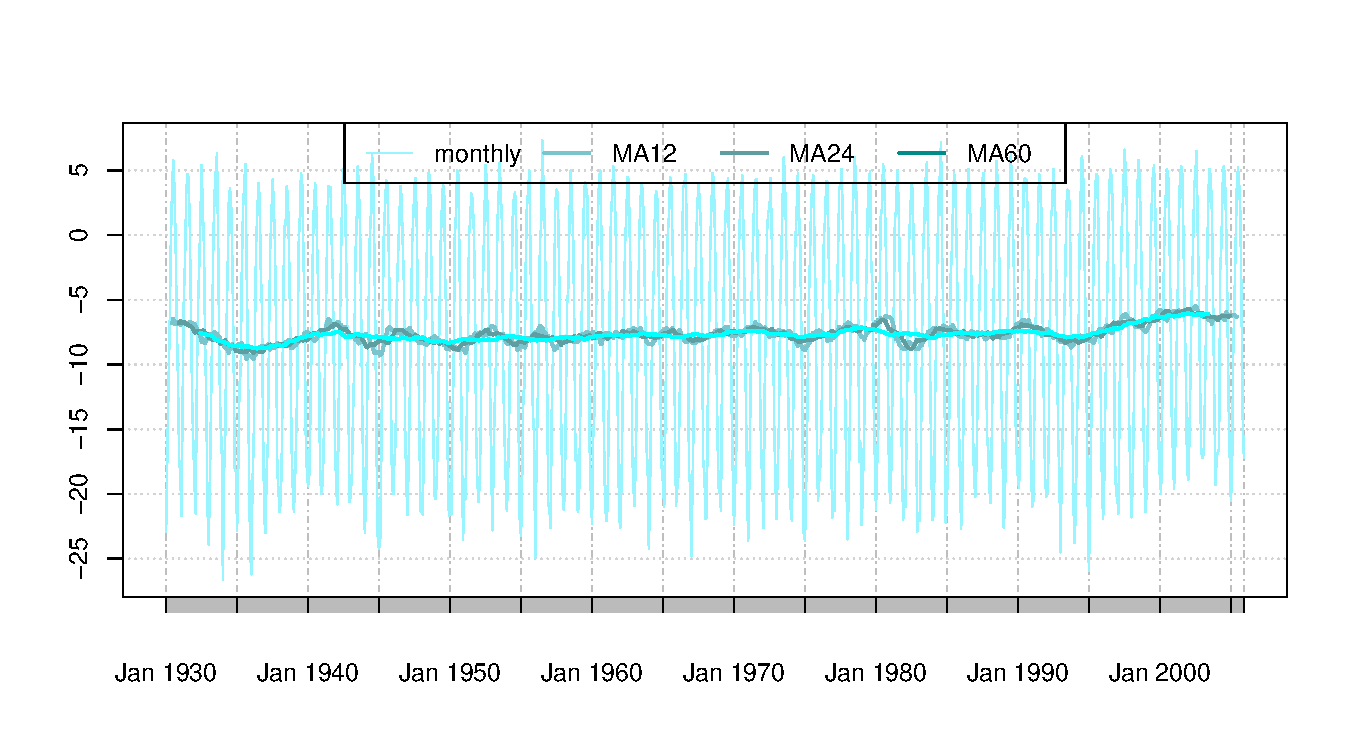
\includegraphics[width=0.9\textwidth]{./externalfig/tiens_ma.pdf}
\end{frame}

%------------------------------------------------------------%

\begin{frame}[fragile]\frametitle{Interpolation of missing values}
\begin{itemize}
\item{\textbf{IMPORTANT!} Interpolation should be applied carefully, since you change your data and you can introduce errors.}
\item{simple methods for interpolation}
    \begin{itemize}
    \item Linear interpolation
\begin{knitrout}
\definecolor{shadecolor}{rgb}{0.961, 0.961, 0.961}\color{fgcolor}\begin{kframe}
\begin{alltt}
\hlkwd{na.approx}\hlstd{(object, ...)}
\end{alltt}
\end{kframe}
\end{knitrout}
    \item Spline interpolation
\begin{knitrout}
\definecolor{shadecolor}{rgb}{0.961, 0.961, 0.961}\color{fgcolor}\begin{kframe}
\begin{alltt}
\hlkwd{na.spline}\hlstd{(object, ...)}
\end{alltt}
\end{kframe}
\end{knitrout}
    \item Last Observation Carried Forward
\begin{knitrout}
\definecolor{shadecolor}{rgb}{0.961, 0.961, 0.961}\color{fgcolor}\begin{kframe}
\begin{alltt}
\hlkwd{na.locf}\hlstd{(object,} \hlkwc{na.rm} \hlstd{=} \hlnum{TRUE}\hlstd{, ...)}
\end{alltt}
\end{kframe}
\end{knitrout}
    \end{itemize}
\item with \rcode{maxgap} you can always specifiy the maximum gap length which should be interpolated. For example with \rcode{maxgap=2} only gaps up to a length of 2 observations woud be interpolated
\end{itemize}
\end{frame}

%------------------------------------------------------------%

\begin{frame}\frametitle{Your turn ...}
  \begin{exercise}{The temperature data of station Fergana} %ex18
  Load the monthly temperature of station Fergana (\texttt{data/Fergana.txt}) or refer to any other station of your choice and do the following steps.
  \begin{enumerate}
  \item Calculate annual minimum, maximum and mean temperatures
  \item Calculate a moving average to smoothen the time series. Use a window length of 12 months.
  \item Merge the monthly temperatures of Ferdana with Tien Shan and plot them. Add the smoothed time series for both time series.
  \item Calculate seasonal mean temperatures (\rcode{period.apply}).
  \item Extra: We cannot compare the global monthly temperature anomalies to the monthly temperature averages of the stations. Why? Create a plot of monthly temperature anomalies.
  \end{enumerate}
  \end{exercise}
  \small{Make sure your working directory is set correctly!}
\end{frame}

%------------------------------------------------------------%

% Daten Stationszeitreihen - Webportale:
% Climate databases:
% \href{http://www.webpages.uidaho.edu/cae/data/cad/gmap.html}{webpages.uidaho.edu/cae/data/cad/gmap} (monthly data series, Central Asia)
% http://nsidc.org/data/docs/noaa/g02174_central_asia_data/index.html (monthly data series, former Soviet Union)
% http://climexp.knmi.nl (global)

%------------------------------------------------------------%

\begin{frame}[fragile]\frametitle{Solution for Exercise \arabic{exercisecount}}
Load the Fergana station data
\begin{knitrout}\footnotesize
\definecolor{shadecolor}{rgb}{0.961, 0.961, 0.961}\color{fgcolor}\begin{kframe}
\begin{alltt}
\hlstd{ferg.orig} \hlkwb{<-} \hlkwd{read.table}\hlstd{(}\hlstr{"data/Fergana.txt"}\hlstd{,} \hlkwc{header}\hlstd{=F,}
                       \hlkwc{skip}\hlstd{=}\hlnum{4}\hlstd{,} \hlkwc{na.strings}\hlstd{=}\hlstr{"-99999"}\hlstd{)}
\hlstd{timerange} \hlkwb{<-} \hlkwd{paste}\hlstd{(}\hlkwd{range}\hlstd{(ferg.orig[,}\hlnum{1}\hlstd{]),} \hlkwd{c}\hlstd{(}\hlstr{"-01-01"}\hlstd{,} \hlstr{"-12-01"}\hlstd{),} \hlkwc{sep}\hlstd{=}\hlstr{""}\hlstd{)}
\hlstd{timerange} \hlkwb{<-} \hlkwd{as.Date}\hlstd{(timerange)}
\hlcom{# create monthly time sequence}
\hlstd{mont} \hlkwb{<-} \hlkwd{as.yearmon}\hlstd{(}\hlkwd{seq}\hlstd{(}\hlkwd{first}\hlstd{(timerange),} \hlkwd{last}\hlstd{(timerange),} \hlkwc{by}\hlstd{=}\hlstr{"month"}\hlstd{))}
\hlstd{tmon.ferg} \hlkwb{<-} \hlkwd{xts}\hlstd{(}\hlkwd{c}\hlstd{(}\hlkwd{t}\hlstd{(ferg.orig[,}\hlopt{-}\hlnum{1}\hlstd{])),} \hlkwc{order.by}\hlstd{=mont)}
\hlkwd{str}\hlstd{(tmon.ferg)}
\end{alltt}
\begin{verbatim}
## An 'xts' object on Jan 1881/Dec 2003 containing:
##   Data: num [1:1476, 1] NA NA NA NA NA NA NA NA NA NA ...
##   Indexed by objects of class: [yearmon] TZ: 
##   xts Attributes:  
##  NULL
\end{verbatim}
\end{kframe}
\end{knitrout}
\end{frame}
  
%------------------------------------------------------------%

\begin{frame}[fragile]\frametitle{Solution for Exercise \arabic{exercisecount}.1}
  \begin{enumerate}
  \item[1.] Calculate annual minimum, maximum and mean temperatures
\begin{knitrout}
\definecolor{shadecolor}{rgb}{0.961, 0.961, 0.961}\color{fgcolor}\begin{kframe}
\begin{alltt}
\hlkwd{apply.yearly}\hlstd{(tmon.ferg,} \hlkwc{FUN}\hlstd{=min)}
\hlkwd{apply.yearly}\hlstd{(tmon.ferg,} \hlkwc{FUN}\hlstd{=max)}
\hlkwd{apply.yearly}\hlstd{(tmon.ferg,} \hlkwc{FUN}\hlstd{=mean)}
\end{alltt}
\end{kframe}
\end{knitrout}
  \end{enumerate}
\end{frame}

%------------------------------------------------------------%

\begin{frame}[fragile]\frametitle{Solution for Exercise \arabic{exercisecount}.2}
  \begin{enumerate}
  \item[2.] Calculate a moving average to smoothen the time series. Use a window length of 12 months.
  \end{enumerate}
\begin{knitrout}
\definecolor{shadecolor}{rgb}{0.961, 0.961, 0.961}\color{fgcolor}\begin{kframe}
\begin{alltt}
\hlstd{tmon.ma.ferg} \hlkwb{<-} \hlkwd{rollapply}\hlstd{(tmon.ferg,} \hlkwc{width}\hlstd{=}\hlnum{12}\hlstd{,} \hlkwc{FUN}\hlstd{=mean)}
\hlkwd{plot}\hlstd{(tmon.ferg,} \hlkwc{type}\hlstd{=}\hlstr{"n"}\hlstd{)}
\hlkwd{lines}\hlstd{(tmon.ferg,} \hlkwc{lwd}\hlstd{=}\hlnum{2}\hlstd{,} \hlkwc{col}\hlstd{=}\hlstr{"grey80"}\hlstd{)}
\hlkwd{lines}\hlstd{(tmon.ma.ferg,} \hlkwc{lwd}\hlstd{=}\hlnum{2}\hlstd{,} \hlkwc{col}\hlstd{=}\hlstr{"darkblue"}\hlstd{)}
\end{alltt}
\end{kframe}

{\centering \includegraphics[width=.9\textwidth]{./fig/fergama-1} 

}



\end{knitrout}
\end{frame}

%------------------------------------------------------------%

\begin{frame}[fragile]\frametitle{Solution for Exercise \arabic{exercisecount}.3}
  \begin{enumerate}
  \item[3.] Merge the monthly temperatures of Ferdana with Tien Shan plot them. Add the smoothed (12) time series for both time series.
  \end{enumerate}
\begin{knitrout}\small
\definecolor{shadecolor}{rgb}{0.961, 0.961, 0.961}\color{fgcolor}\begin{kframe}
\begin{alltt}
\hlcom{# merge the monthly data}
\hlstd{tmon} \hlkwb{<-} \hlkwd{merge}\hlstd{(}\hlkwc{FERGANA}\hlstd{=tmon.ferg,} \hlkwc{TIENSHAN}\hlstd{=}\hlkwd{as.xts}\hlstd{(tmon.tiens))}
\hlcom{# calculate smoothing for Tien Shan}
\hlstd{tmon.ma.tiens} \hlkwb{<-} \hlkwd{rollapply}\hlstd{(tmon.tiens,} \hlkwc{width}\hlstd{=}\hlnum{12}\hlstd{,} \hlkwc{FUN}\hlstd{=mean)}
\hlcom{# merge with the monthly data}
\hlstd{tmon} \hlkwb{<-} \hlkwd{merge}\hlstd{(tmon,} \hlkwc{FERGANAma}\hlstd{=tmon.ma.ferg)}
\hlstd{tmon} \hlkwb{<-} \hlkwd{merge}\hlstd{(tmon,} \hlkwc{TIENSHANma}\hlstd{=}\hlkwd{as.xts}\hlstd{(tmon.ma.tiens))}
\end{alltt}
\end{kframe}
\end{knitrout}
\end{frame}

%------------------------------------------------------------%


\begin{frame}[fragile]\frametitle{Solution for Exercise \arabic{exercisecount}.3}
\begin{knitrout}\scriptsize
\definecolor{shadecolor}{rgb}{0.961, 0.961, 0.961}\color{fgcolor}\begin{kframe}
\begin{alltt}
\hlkwd{str}\hlstd{(tmon,} \hlkwc{vec.len}\hlstd{=}\hlnum{2}\hlstd{)}
\end{alltt}
\begin{verbatim}
## An 'xts' object on Jan 1881/Dec 2005 containing:
##   Data: num [1:1500, 1:4] NA NA NA NA NA NA NA NA NA NA ...
##  - attr(*, "dimnames")=List of 2
##   ..$ : NULL
##   ..$ : chr [1:4] "FERGANA" "TIENSHAN" "FERGANAma" "TIENSHANma"
##   Indexed by objects of class: [yearmon] TZ: 
##   xts Attributes:  
##  NULL
\end{verbatim}
\end{kframe}
\end{knitrout}
\end{frame}

%------------------------------------------------------------%

\begin{frame}[fragile]\frametitle{Solution for Exercise \arabic{exercisecount}.3}

\begin{knitrout}\scriptsize
\definecolor{shadecolor}{rgb}{0.961, 0.961, 0.961}\color{fgcolor}\begin{kframe}
\begin{alltt}
\hlkwd{plot}\hlstd{(tmon[,}\hlnum{1}\hlstd{],} \hlkwc{ylim}\hlstd{=}\hlkwd{range}\hlstd{(tmon,} \hlkwc{na.rm}\hlstd{=T),} \hlkwc{type}\hlstd{=}\hlstr{"n"}\hlstd{,} \hlkwc{main}\hlstd{=}\hlstr{""}\hlstd{)}
\hlkwd{suppressWarnings}\hlstd{(mycol} \hlkwb{<-} \hlkwd{c}\hlstd{(}\hlkwd{addAlpha}\hlstd{(}\hlstr{"deepskyblue"}\hlstd{,} \hlkwd{c}\hlstd{(}\hlnum{.5}\hlstd{,}\hlnum{1}\hlstd{)),}
                            \hlkwd{addAlpha}\hlstd{(}\hlstr{"firebrick3"}\hlstd{,}  \hlkwd{c}\hlstd{(}\hlnum{.5}\hlstd{,}\hlnum{1}\hlstd{))))}
\hlkwd{lines}\hlstd{(tmon[,}\hlnum{1}\hlstd{],} \hlkwc{col}\hlstd{=mycol[}\hlnum{1}\hlstd{]);} \hlkwd{lines}\hlstd{(tmon[,}\hlnum{2}\hlstd{],} \hlkwc{col}\hlstd{=mycol[}\hlnum{3}\hlstd{])}
\hlkwd{lines}\hlstd{(tmon[,}\hlnum{3}\hlstd{],} \hlkwc{col}\hlstd{=mycol[}\hlnum{2}\hlstd{],} \hlkwc{lwd}\hlstd{=}\hlnum{2}\hlstd{);}
\hlkwd{lines}\hlstd{(tmon[,}\hlnum{4}\hlstd{],} \hlkwc{col}\hlstd{=mycol[}\hlnum{4}\hlstd{],} \hlkwc{lwd}\hlstd{=}\hlnum{2}\hlstd{)}
\hlkwd{legend}\hlstd{(}\hlstr{"bottomleft"}\hlstd{,} \hlkwd{c}\hlstd{(}\hlstr{"Fergana, monthly"}\hlstd{,}\hlstr{"moving average"}\hlstd{,}\hlstr{"Tien Shan, monthly"}\hlstd{,}
\hlstr{"moving average"}\hlstd{),} \hlkwc{col}\hlstd{=mycol,} \hlkwc{bg}\hlstd{=}\hlstr{"transparent"}\hlstd{,} \hlkwc{lwd}\hlstd{=}\hlkwd{c}\hlstd{(}\hlnum{1}\hlstd{,}\hlnum{2}\hlstd{),} \hlkwc{ncol}\hlstd{=}\hlnum{2}\hlstd{)}
\end{alltt}
\end{kframe}

{\centering \includegraphics[width=.8\textwidth]{./fig/fergmergeplot-1} 

}



\end{knitrout}
\end{frame}

%------------------------------------------------------------%

\begin{frame}[fragile]\frametitle{Solution for Exercise \arabic{exercisecount}.4}
  \begin{enumerate}
  \item[4.] Calculate seasonal mean temperatures for spring, summer, autumn and winter (\rcode{period.apply}).
  \end{enumerate}
\begin{knitrout}\small
\definecolor{shadecolor}{rgb}{0.961, 0.961, 0.961}\color{fgcolor}\begin{kframe}
\begin{alltt}
\hlcom{# quarterly means}
\hlkwd{apply.quarterly}\hlstd{(tmon.ferg, mean)}\hlcom{# not adapted to seasons}
\hlcom{# We have do that manually}
\hlstd{btime} \hlkwb{<-} \hlkwd{format}\hlstd{(}\hlkwd{time}\hlstd{(tmon.ferg),} \hlstr{"%b"}\hlstd{)}
\hlstd{seas.index} \hlkwb{<-} \hlkwd{c}\hlstd{(}\hlnum{0}\hlstd{,} \hlkwd{which}\hlstd{(btime} \hlopt \hlkwd{c}\hlstd{(}\hlstr{"Feb"}\hlstd{,}\hlstr{"May"}\hlstd{,}\hlstr{"Aug"}\hlstd{,}\hlstr{"Nov"}\hlstd{)))}
\hlcom{# last months per season: djF, amM, jjA, soN}
\hlstd{seas.mean} \hlkwb{<-} \hlkwd{period.apply}\hlstd{(tmon.ferg,} \hlkwc{INDEX}\hlstd{=seas.index,} \hlkwc{FUN}\hlstd{=mean)}
\hlcom{##  we have to rejoin the time information}
\hlstd{seas.mean} \hlkwb{<-} \hlkwd{xts}\hlstd{(seas.mean[,}\hlnum{1}\hlstd{],}
                 \hlkwc{order.by}\hlstd{=}\hlkwd{time}\hlstd{(tmon.ferg)[seas.index])}
\end{alltt}
\end{kframe}
\end{knitrout}
\end{frame}

%------------------------------------------------------------%
%------------------------------------------------------------%
\subsection{Trend analysis of time series}
%------------------------------------------------------------%
%------------------------------------------------------------%

% trend in general
% decompose(empirical)
% wavelet, ssa to remove noise
% linear trend
% global T anom

%------------------------------------------------------------%

\begin{frame}[fragile]\frametitle{Trend in the global annual mean temperature anomalies}
Plot global annual mean temperatures with a moving average, a local polynomial regression fit and a linear trend
\begin{knitrout}
\definecolor{shadecolor}{rgb}{0.961, 0.961, 0.961}\color{fgcolor}\begin{kframe}
\begin{alltt}
\hlstd{anngt.zoo} \hlkwb{<-} \hlkwd{as.zoo}\hlstd{(globtemp.annual)}
\hlkwd{plot}\hlstd{(anngt.zoo)}
\hlstd{anngt.lm} \hlkwb{<-} \hlkwd{lm}\hlstd{(anngt.zoo} \hlopt{~} \hlkwd{time}\hlstd{(anngt.zoo))}
\hlkwd{abline}\hlstd{(anngt.lm)}
\hlkwd{lines}\hlstd{(}\hlkwd{time}\hlstd{(anngt.zoo),} \hlkwd{predict}\hlstd{(anngt.lm))}
\hlkwd{lines}\hlstd{(}\hlkwd{time}\hlstd{(anngt.zoo),} \hlkwd{predict}\hlstd{(}\hlkwd{loess}\hlstd{(anngt.zoo} \hlopt{~}
                                \hlkwd{time}\hlstd{(anngt.zoo))))}
\hlstd{anngtma.zoo} \hlkwb{<-} \hlkwd{rollapply}\hlstd{(anngt.zoo,}\hlnum{31}\hlstd{, mean)}
\hlkwd{lines}\hlstd{(}\hlkwd{time}\hlstd{(anngtma.zoo), anngtma.zoo)}
\end{alltt}
\end{kframe}
\end{knitrout}
\end{frame}

%------------------------------------------------------------%



%------------------------------------------------------------%

\begin{frame}[fragile]\frametitle{Assessing trend in the global annual temperature anomaly time series}
The climate is variable and therefore trend analysis complex
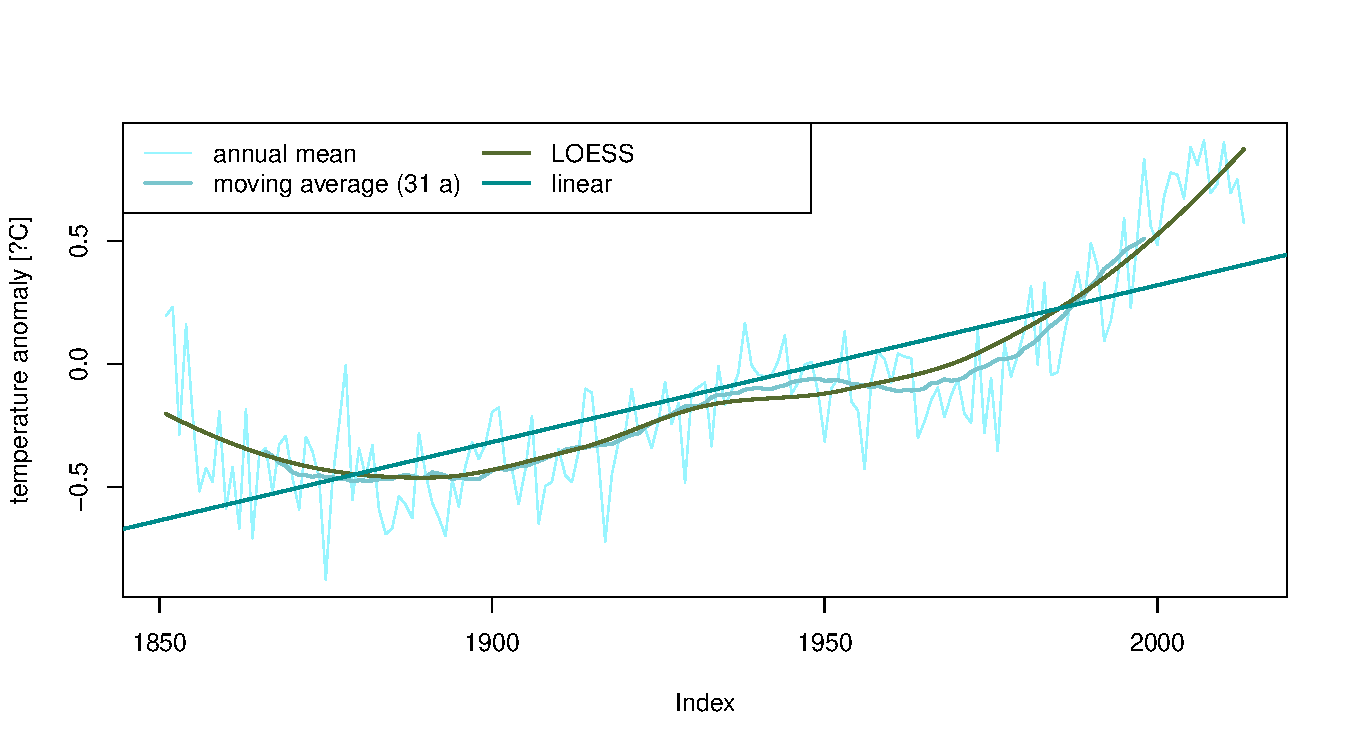
\includegraphics[width=0.9\textwidth]{./externalfig/globalannt_trend.pdf}
\end{frame}

%------------------------------------------------------------%

\begin{frame}[fragile]\frametitle{Linear model for testing of a trend in time series}
Linear models are not the best choice
\begin{itemize}
\item when there is autocorrelation in the time series
\item linear models assume independence of residuals
\item trends don't have to be linear 
\end{itemize}
\end{frame}

%------------------------------------------------------------%

\begin{frame}\frametitle{Nonparametric methods for trend analysis}
\begin{figure}[H]
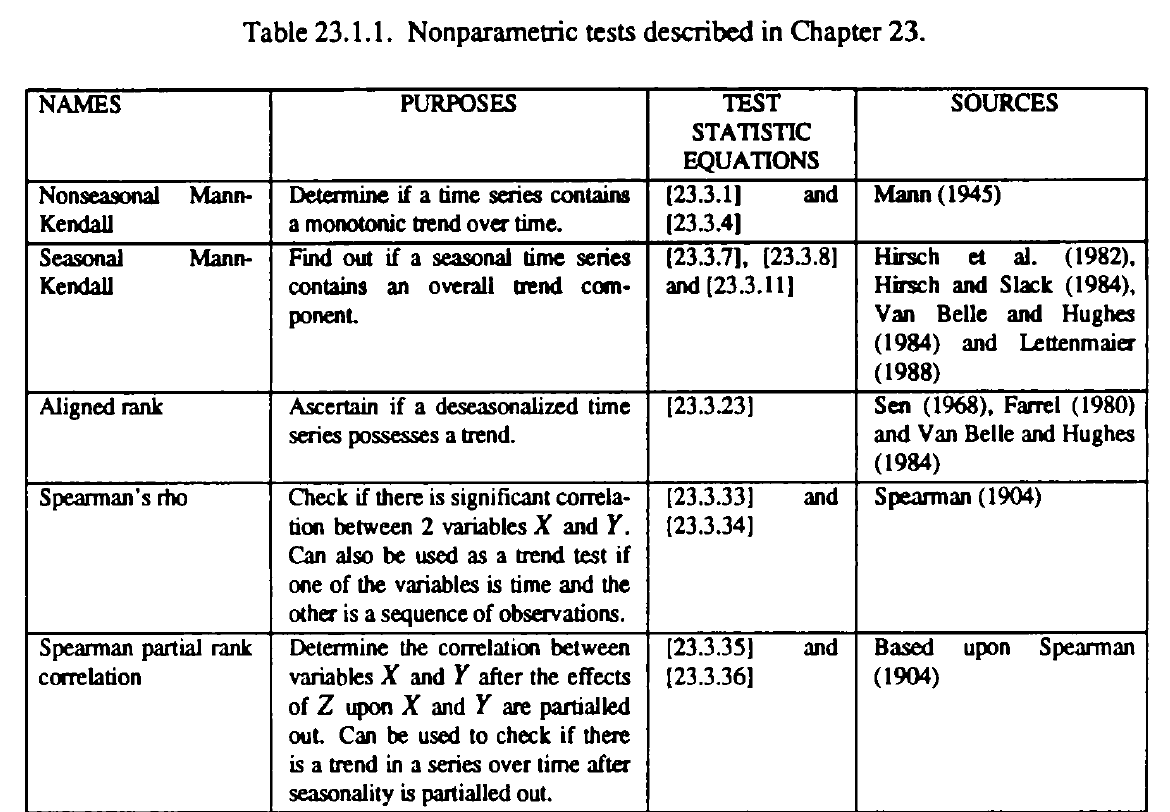
\includegraphics[width=0.8\textwidth]{externalfig/nonparametrictrend_tab_hipel94.png}\\
\begin{flushright}\tiny{from cite{Hipel1994}}\end{flushright} %need a proper CITE here
\end{figure}
\end{frame}

%------------------------------------------------------------%

\begin{frame}\frametitle{Nonparametric methods for trend analysis}
Wikipedia:
\begin{quote}
"In statistics, the term non-parametric statistics refers to statistics that do not assume the data or population have any characteristic structure or parameters."
\end{quote}
\begin{itemize}
\item{For example, this means there are no assumptions made regarding the sample distribution}
\item nonparametric methods are often designed for nominally or ordinally scaled variables
\end{itemize}
\end{frame}

%------------------------------------------------------------%

\begin{frame}[fragile]\frametitle{The Mann-Kendall test}
theoretical basis of Mann-Kendall
\begin{description}
 \item[$H_0$:] {data is from a population of random independent variables}
 \item[$H_1$:] {data follows a monotonic trend}
\end{description}
cite{Hipel1994}
\end{frame}

%------------------------------------------------------------%

\begin{frame}[fragile]\frametitle{The Mann-Kendall test statistic}
Mann-Kendall test statistic is
\[ S = \sum_{k=1}^{n-1} \sum_{j=k+1}^{n} sgn(x_j -x_k)\]
where
 \[
sgn(x)=\begin{cases}
              1 & x>0\\
              0 & x=0\\
              -1 & x<0
              \end{cases}
 \]
 As a result, the time series is transformed to a series of 1,0,-1 and $S$ is asymptotically normally distributed.
\end{frame}

%------------------------------------------------------------%

\begin{frame}[fragile]\frametitle{The Mann-Kendall test}
\begin{description}
\item[Positive values] for $S$ result in a postive trend
\item[Negative values] for $S$ result in a negative trend
\end{description}
\begin{itemize}
\item If $S$ is significantly different from 0, then there is a trend.
\item The Kendall $\tau$ is related to $S$ so the significance can be calculated 
\item The Mann-Kendall test is applicable for annual data, there are adaptions to deal with seasonal variation, though.
\end{itemize}
\end{frame}

%------------------------------------------------------------%

\begin{frame}[fragile]\frametitle{The Mann-Kendall test for global annual mean temperature anomalies}
The Mann-Kendall test is implemented in the package \rcode{Kendall}
\begin{knitrout}
\definecolor{shadecolor}{rgb}{0.961, 0.961, 0.961}\color{fgcolor}\begin{kframe}
\begin{alltt}
\hlcom{# package for the test}
\hlkwd{library}\hlstd{(Kendall)}
\hlcom{# execution of test}
\hlkwd{MannKendall}\hlstd{(anngt.zoo)}
\end{alltt}
\begin{verbatim}
## tau = 0.595, 2-sided pvalue =< 2.22e-16
\end{verbatim}
\end{kframe}
\end{knitrout}
The low p value indicates that the $H_0$ was rejected - there is a significant trend.
\end{frame}

%------------------------------------------------------------%

\begin{frame}[fragile]\frametitle{Assessing trend in the global annual temperature anomaly time series}
The test highlights the clear trend 
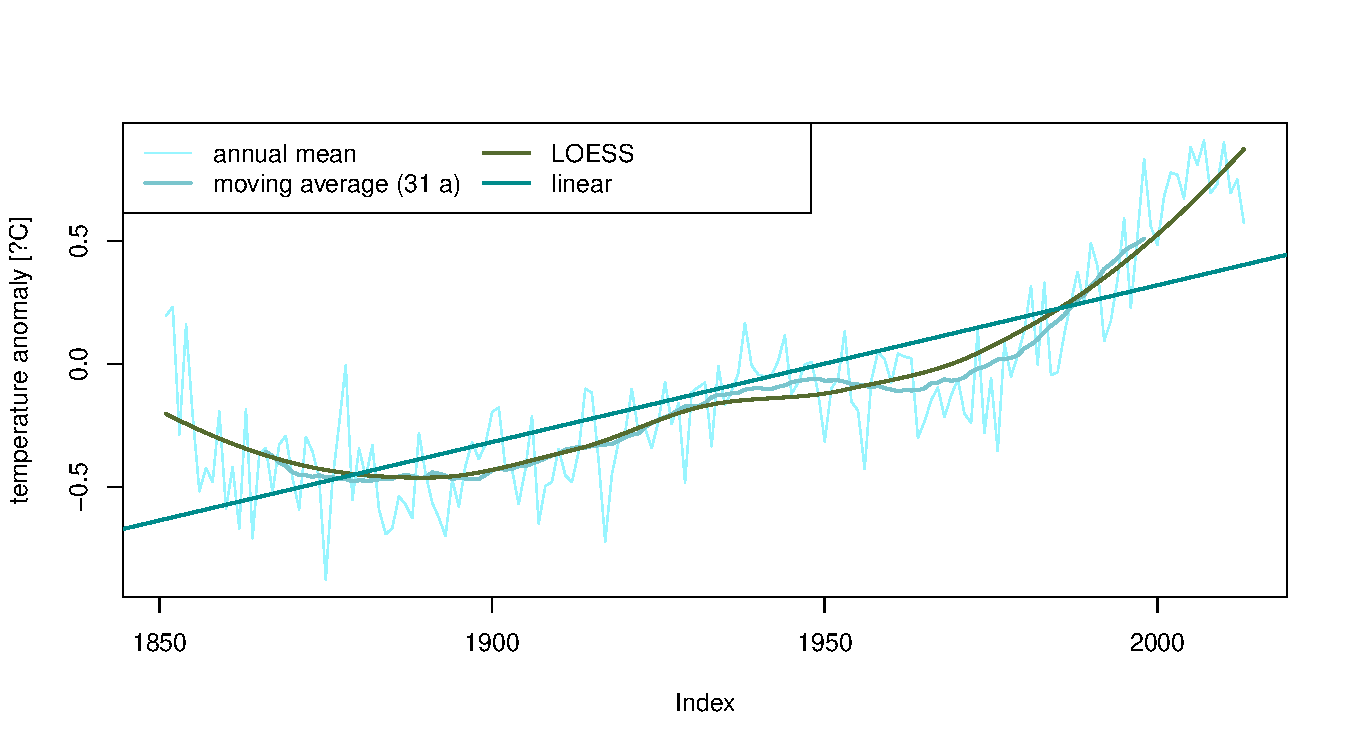
\includegraphics[width=0.9\textwidth]{./externalfig/globalannt_trend.pdf}
\end{frame}

%------------------------------------------------------------%

\begin{frame}[fragile]\frametitle{Your turn ...}
\begin{exercise}{Trendanalysis of the Tien Shan dataset} %ex19
Analyse if there is a significant trend in the Tien Shan time series. Compare different periods of the record.
\end{exercise}
\end{frame}

%------------------------------------------------------------%

\begin{frame}[fragile]\frametitle{Solution for exercise \arabic{exercisecount}}
It seems that the temperature started to increase in the 70ies. Was there a significant trend before? This time we use an improved test that returns more information, called Yue Pilon method of computing nonlinear prewhitened trends.
\begin{knitrout}
\definecolor{shadecolor}{rgb}{0.961, 0.961, 0.961}\color{fgcolor}\begin{kframe}
\begin{alltt}
\hlcom{# load the package}
\hlkwd{library}\hlstd{(zyp)}
\hlcom{# execution of test: zyp.yuepilon}
\end{alltt}
\end{kframe}
\end{knitrout}
\end{frame}
%------------------------------------------------------------%

\begin{frame}[fragile]\frametitle{The Mann-Kendall test for global annual mean temperature anomalies}
\begin{knitrout}\footnotesize
\definecolor{shadecolor}{rgb}{0.961, 0.961, 0.961}\color{fgcolor}\begin{kframe}
\begin{alltt}
\hlkwd{zyp.yuepilon}\hlstd{(anngt.zoo[}\hlkwd{time}\hlstd{(anngt.zoo)} \hlopt{<} \hlnum{1970}\hlstd{],}
             \hlkwc{conf.intervals}\hlstd{=}\hlnum{TRUE}\hlstd{)}
\end{alltt}
\begin{verbatim}
##        lbound         trend 
##  2.982143e-03  3.992063e-03 
##        trendp        ubound 
##  4.750556e-01  4.983333e-03 
##           tau           sig 
##  3.078372e-01  8.344650e-07 
##         nruns       autocor 
##  1.000000e+00  4.170353e-01 
##    valid_frac        linear 
##  1.000000e+00  3.353850e-03 
##     intercept 
## -5.221111e-01
\end{verbatim}
\end{kframe}
\end{knitrout}
The low p value indicates that the $H_0$ was rejected - there was a significant trend already before 1970.
\end{frame}

%------------------------------------------------------------%

\begin{frame}\frametitle{Variability of the temperature trend at the station Tien Shan}
cite{katy2013} showed that the test result is affected by the chosen period.
\begin{figure}[H]
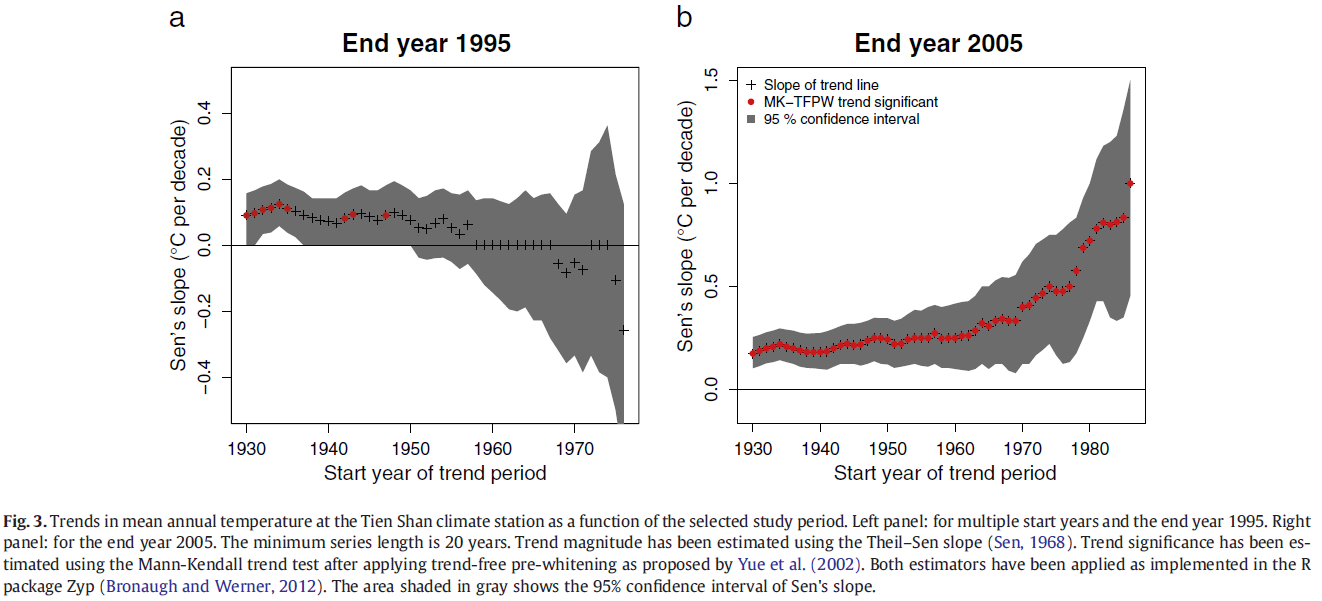
\includegraphics[width=0.9\textwidth]{externalfig/Trend_TienShan_katy2013.png}\\
\begin{flushright}\tiny{from cite{katy2013}}\end{flushright} %need a proper CITE here
\end{figure}
\end{frame}

%------------------------------------------------------------%

\begin{frame}[fragile]\frametitle{Climate projection with a weather generator}
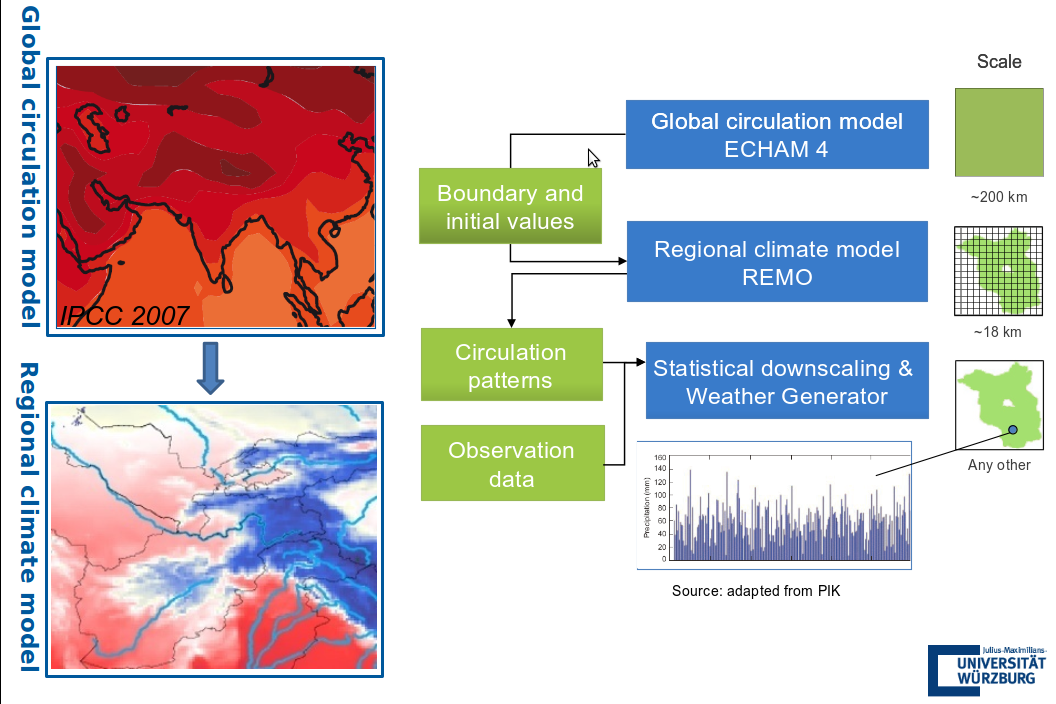
\includegraphics[width=0.9\textwidth]{./externalfig/remo_screenshot}
\end{frame}

%------------------------------------------------------------%

\begin{frame}[fragile]\frametitle{Your turn ...}
 \begin{exercise}{Analysis of a REMO climate projection of Fergana station} %ex20
In this exercise we will work with the projected climate data of REMO. The REMO data is saved within the file \texttt{remo\_t2m\_CAstations.dat}. The time series is regular and extends from 1.1.1950 to 31.12.2100.
\begin{enumerate}
\item Read the data and extract the 75th temperature data column which contains the Fergana data. This a large file and if your computer is slow, please skip this step. The reason is that the file is big and it asks you to read 226 * 55153 = 12464578 data points. To do this ask the teachers for help.
\item Calculate annual means and plot the result. What do you see?
\item Calculate climatology (means per every month) for the past (before 2000), the near future (until 2050) and the far future (after 2050) and display. What do you see?
\end{enumerate}
\end{exercise}
\end{frame}

%------------------------------------------------------------%

\begin{frame}[fragile]\frametitle{Help on exercise \arabic{exercisecount}.1}
\begin{enumerate}
\item use \rcode{read.table} to read the file
\item retrieve the temporal information from the rownames with \rcode{as.Date}
\item create a xts class object
\end{enumerate}
\end{frame}

%------------------------------------------------------------%

\begin{frame}[fragile]\frametitle{Help on exercise \arabic{exercisecount}.2}
\begin{enumerate}
\item Use \rcode{apply.yearly} for the calculation of annual means.
\item For plotting you can just use the standard \rcode{plot}ting command.
\end{enumerate}
\end{frame}

%------------------------------------------------------------%

\begin{frame}[fragile]\frametitle{Help on exercise \arabic{exercisecount}.3}
Congratulations for making it to this point!
\begin{enumerate}
\item Calculate monthly means with with \rcode{apply.monthly}.
\item Create a \rcode{data.frame} that contains three columns named
\begin{description}
\item[T2m] {the monthly temperature means of Fergana}
\item[MONTH] {the names of the months as created by \rcode{format(YOUR TIME, format="\%b")}, saved as ordered factors}
\item[PERIOD] {the periods "past", "near future" and "far future" as factors}
\end{description}
\item For plotting you can then use the elegant \rcode{bwplot(data=YOUR DATA NAME, T2m $\sim$  MONTH \textbar PERIOD)} command.
\end{enumerate}
\end{frame}

%------------------------------------------------------------%

\begin{frame}[fragile]\frametitle{Attention!}
The following solutions are not a perfect example of the best statistical approach to analyse REMO data. It is just an exercise for us to practice.
\end{frame}

%------------------------------------------------------------%

\begin{frame}[fragile]\frametitle{Solution for exercise \arabic{exercisecount}.1}
\begin{knitrout}
\definecolor{shadecolor}{rgb}{0.961, 0.961, 0.961}\color{fgcolor}\begin{kframe}
\begin{alltt}
\hlcom{# use read.table to read the file}
\hlstd{allremo} \hlkwb{<-} \hlkwd{read.table}\hlstd{(}\hlstr{"data/remo_T2m_CAstations.dat"}\hlstd{)}
\hlcom{# retrieve the temporal information from the rownames}
\hlstd{times} \hlkwb{<-} \hlkwd{as.Date}\hlstd{(}\hlkwd{rownames}\hlstd{(allremo),} \hlkwc{format}\hlstd{=}\hlstr{"%d%m%Y"}\hlstd{)}
\hlcom{# create a xts class object}
\hlstd{ferremo} \hlkwb{<-} \hlkwd{xts}\hlstd{(allremo[,}\hlnum{75}\hlstd{], times)}
\end{alltt}
\end{kframe}
\end{knitrout}
\small at this point remove unneccessary data with \rcode{rm(allremo); gc()}
% <<saveferremo, include=FALSE, eval=FALSE>>=
%  save(ferremo, file="data/fergana_remo.Rdata")
% @

\end{frame}

%------------------------------------------------------------%

\begin{frame}[fragile]\frametitle{Solution for exercise \arabic{exercisecount}.2}
\begin{knitrout}
\definecolor{shadecolor}{rgb}{0.961, 0.961, 0.961}\color{fgcolor}\begin{kframe}
\begin{alltt}
\hlstd{annferremo} \hlkwb{<-} \hlkwd{apply.yearly}\hlstd{(ferremo, mean)}
\hlkwd{plot}\hlstd{(annferremo)}
\end{alltt}
\end{kframe}

{\centering \includegraphics[width=.8\textwidth]{./fig/remoanalysis2-1} 

}



\end{knitrout}
\end{frame}

%------------------------------------------------------------%

\begin{frame}[fragile]\frametitle{Solution for exercise \arabic{exercisecount}.3}
\begin{knitrout}\footnotesize
\definecolor{shadecolor}{rgb}{0.961, 0.961, 0.961}\color{fgcolor}\begin{kframe}
\begin{alltt}
\hlstd{monferremo} \hlkwb{<-} \hlkwd{apply.monthly}\hlstd{(ferremo, mean)}
\hlstd{monferremo.df} \hlkwb{<-} \hlkwd{data.frame}\hlstd{(}\hlkwc{T2m}\hlstd{=}\hlkwd{as.numeric}\hlstd{(monferremo),}
                    \hlkwc{MONTH}\hlstd{=}\hlkwd{format}\hlstd{(}\hlkwd{time}\hlstd{(monferremo),} \hlstr{"%b"}\hlstd{),} \hlkwc{PERIOD}\hlstd{=}\hlnum{1}\hlstd{)}
\hlstd{monferremo.df}\hlopt{$}\hlstd{PERIOD[} \hlkwd{time}\hlstd{(monferremo)} \hlopt{>} \hlkwd{as.Date}\hlstd{(}\hlstr{"2000-01-01"}\hlstd{)]} \hlkwb{<-} \hlnum{2}
\hlstd{monferremo.df}\hlopt{$}\hlstd{PERIOD[} \hlkwd{time}\hlstd{(monferremo)} \hlopt{>} \hlkwd{as.Date}\hlstd{(}\hlstr{"2050-01-01"}\hlstd{)]} \hlkwb{<-} \hlnum{3}
\hlstd{monferremo.df}\hlopt{$}\hlstd{PERIOD} \hlkwb{<-} \hlkwd{factor}\hlstd{(monferremo.df}\hlopt{$}\hlstd{PERIOD,}
        \hlkwc{labels}\hlstd{=}\hlkwd{c}\hlstd{(}\hlstr{"past"}\hlstd{,} \hlstr{"near future"}\hlstd{,} \hlstr{"far future"}\hlstd{))}
\hlstd{monferremo.df}\hlopt{$}\hlstd{MONTH} \hlkwb{<-} \hlkwd{ordered}\hlstd{(monferremo.df}\hlopt{$}\hlstd{MONTH,}
 \hlkwd{c}\hlstd{(}\hlstr{"Jan"}\hlstd{,} \hlstr{"Feb"}\hlstd{,} \hlstr{"Mar"}\hlstd{,} \hlstr{"Apr"}\hlstd{,} \hlstr{"May"}\hlstd{,} \hlstr{"Jun"}\hlstd{,} \hlstr{"Jul"}\hlstd{,}
   \hlstr{"Aug"}\hlstd{,} \hlstr{"Sep"}\hlstd{,}\hlstr{"Oct"}\hlstd{,} \hlstr{"Nov"}\hlstd{,} \hlstr{"Dec"}\hlstd{))}
\end{alltt}
\end{kframe}
\end{knitrout}
\end{frame}

%------------------------------------------------------------%

\begin{frame}[fragile]\frametitle{Solution for exercise \arabic{exercisecount}.3}
\begin{knitrout}
\definecolor{shadecolor}{rgb}{0.961, 0.961, 0.961}\color{fgcolor}\begin{kframe}
\begin{alltt}
\hlkwd{library}\hlstd{(lattice)}
\hlkwd{bwplot}\hlstd{(}\hlkwc{data}\hlstd{=monferremo.df, T2m} \hlopt{~} \hlstd{MONTH} \hlopt{|} \hlstd{PERIOD)}
\end{alltt}
\end{kframe}

{\centering \includegraphics[width=.8\textwidth]{./fig/remoanalysis3a-1} 

}



\end{knitrout}
\end{frame}

%------------------------------------------------------------%

\begin{frame}[fragile]\frametitle{Solution for exercise \arabic{exercisecount}.3}
\begin{knitrout}
\definecolor{shadecolor}{rgb}{0.961, 0.961, 0.961}\color{fgcolor}\begin{kframe}
\begin{alltt}
\hlkwd{bwplot}\hlstd{(}\hlkwc{data}\hlstd{=monferremo.df, T2m} \hlopt{~} \hlstd{PERIOD} \hlopt{|} \hlstd{MONTH)}
\end{alltt}
\end{kframe}

{\centering \includegraphics[width=.8\textwidth]{./fig/remoanalysis3b-1} 

}



\end{knitrout}
\end{frame}

%------------------------------------------------------------%
% 
% <<remoanalysis2_b>>=
% # monthly acf
% monferremo <- apply.monthly(ferremo, mean)
% time(monferremo) <- as.yearmon(time(monferremo))
% pasttmon.ferg <- tmon.ferg[time(tmon.ferg) >= as.yearmon( "Jan 1950") & time(tmon.ferg) < as.yearmon( "Jan 2000")]
% # quick and dirty interpolation of missing values (do not try this at home!)
% pasttmon.ferg <- na.approx(pasttmon.ferg)
% pastmonferremo <- monferremo[time(monferremo) >= as.yearmon( "Jan 1950") & time(monferremo) < as.yearmon( "Jan 2000")]
% par(mfrow=c(2,2))
% acf(pasttmon.ferg)
% pacf(pasttmon.ferg)
% acf(pastmonferremo)
% pacf(pastmonferremo)
% @
% 
%------------------------------------------------------------%

\begin{frame}[fragile]\frametitle{Summary: Methods for time series}

\begin{table}
  \begin{center}
	\label{tab:ts_methods}
	\begin{tabular}{ll}
		\toprule
		Function & description \\
		\midrule
		strptime &  read various time formats \\
		as.POSIXct & convert a time format to the POSIXct format \\
    period.apply& apply a function to number of periods\\
    apply.monthly& monthwise application of a function\\
    aggregate& aggregation for the \rcode{ts} class or \rcode{data.frames}\\
    merge& merge two time series\\
    na.approx & linear interpolation of missing values\\
    na.trim& remove leading and tailing NAs\\
    rollapply & apply a function to window which is slided \\
    & along the time series\\
		\bottomrule
	\end{tabular}
  \end{center}
\end{table}
\end{frame}

%------------------------------------------------------------%
%------------------------------------------------------------%
%\subsection{Packages for managing time series}
%------------------------------------------------------------%
%------------------------------------------------------------%

\begin{frame}[fragile]\frametitle{Time series Summary} 
You learned
\begin{itemize}
\item about linear models in R
\item about a few time series classes and related packages
\item how to import and create time and time series objects
\item how to aggregate
\item how to calculate a running mean
\item how to merge time series
\item how to fit a linear regression
\item how to analyse the regression fit
\item how to perform the Mann-Kendall test
\end{itemize}
\end{frame}

%------------------------------------------------------------%
%------------------------------------------------------------%
\section{Spatial data and GIS functionality}
%------------------------------------------------------------%
%------------------------------------------------------------%

%------------------------------------------------------------%
%------------------------------------------------------------%
\subsection{Spatial Intro}
%------------------------------------------------------------%
%------------------------------------------------------------%

\begin{frame}\frametitle{Authorship note} 
% make note to first slide clickable.
This section (spatial data / GIS) was originally written by Matthias Seibert (see note on the first slide). I heavily borrowed from his slides and wish to thankfully acknowledge his work!
\end{frame}

%------------------------------------------------------------%

\begin{frame}[fragile]\frametitle{GIS functionality of R}
\begin{itemize}[<+->]
\item advanced topic, not one of the core topics
\item substantial functionality is there, see the \href{http://cran.r-project.org/web/views/Spatial.html}{spatial task view}
\item interfaces to SAGA GIS, GRASS, combination
\item there could be a single course about open source GIS:\\ \textbf{ARCGIS prison break}
\end{itemize}
\end{frame}

%------------------------------------------------------------%

\begin{frame}[fragile]\frametitle{GIS functionality of R}
Basically, R is used for almost everything ...
\begin{knitrout}
\definecolor{shadecolor}{rgb}{0.961, 0.961, 0.961}\color{fgcolor}\begin{kframe}
\begin{alltt}
\hlkwd{library}\hlstd{(fortunes)}
\hlstd{oo} \hlkwb{<-} \hlkwd{options}\hlstd{(}\hlkwc{width}\hlstd{=}\hlnum{60}\hlstd{)}
\hlkwd{fortune}\hlstd{(}\hlstr{"only how"}\hlstd{)}
\end{alltt}
\begin{verbatim}
## 
## Evelyn Hall: I would like to know how (if) I can extract
## some of the information from the summary of my nlme.
## Simon Blomberg: This is R. There is no if. Only how.
##    -- Evelyn Hall and Simon 'Yoda' Blomberg
##       R-help (April 2005)
\end{verbatim}
\begin{alltt}
\hlkwd{options}\hlstd{(oo)}
\end{alltt}
\end{kframe}
\end{knitrout}
\end{frame}

%------------------------------------------------------------%

\begin{frame}[fragile]\frametitle{How convinced are R enthusiasts about R as a GIS?}
  Last year I attended a VERY recommendable course (\href{http://geostat-course.org/}{geostat-course.org}) for the promotion of statistical analysis of spatial and spatio-temporal data using open source / free GIS tools. We did the following poll:
  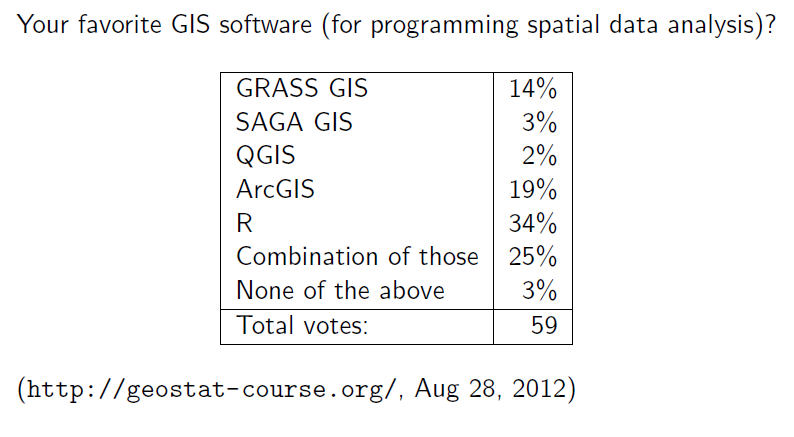
\includegraphics[width=0.8\textwidth]{./externalfig/GEOSTAT_poll.png}
\end{frame}

%------------------------------------------------------------%

\begin{frame}[fragile]\frametitle{Good resources to learn how to use R as a GIS}
\begin{itemize}[<+->]
\item UseR series: Applied Spatial Data Analysis (cite{Bivand2008})
\item package manuals for: \rcode{sp}, \rcode{raster}, \rcode{spacetime}
\item and especially the vignettes of \rcode{sp}, \rcode{raster}, \rcode{spacetime}
\end{itemize}
\end{frame}

%------------------------------------------------------------%

\begin{frame}[fragile]\frametitle{Spatial data}
Spatial data refresher:\\
\begin{center}
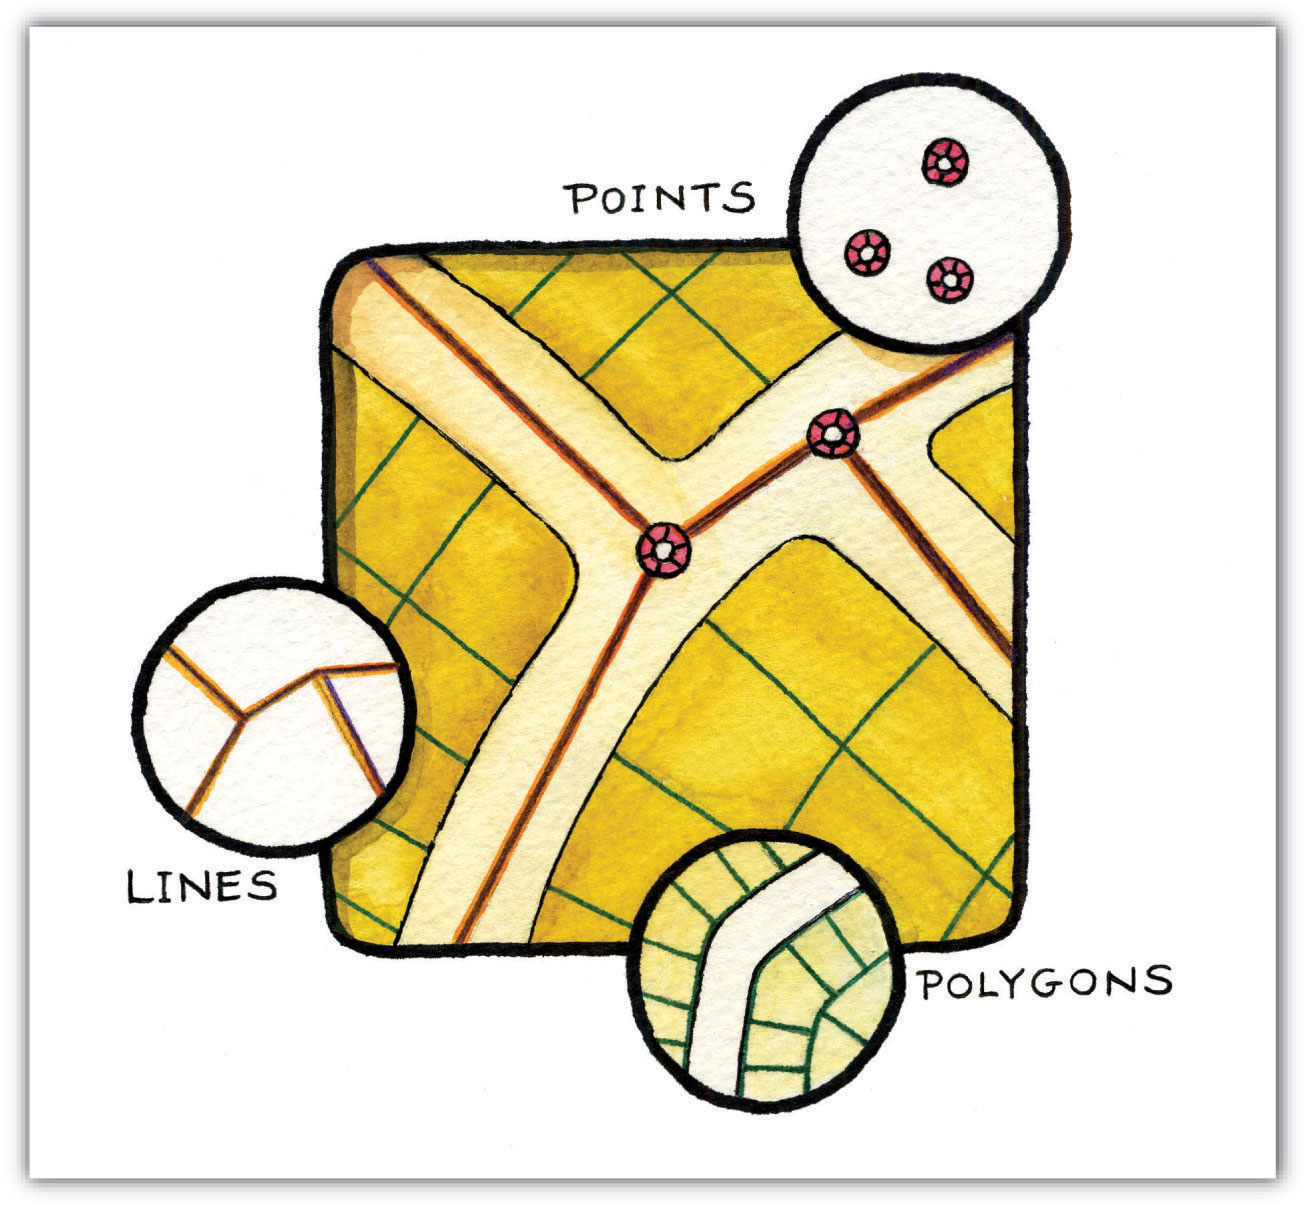
\includegraphics[width=0.5\textwidth]{./externalfig/gis_datatypes.jpg}
\end{center}
\end{frame}

%------------------------------------------------------------%

\begin{frame}[fragile]\frametitle{Spatial data}
Spatial data refresher:
\begin{itemize}[<+->]
\item points, lines, polygons, grids
\item storage: shapefiles, grid files, in- or out-of-memory
\item data bases (e.g. PostGIS): geometry + attributes
\item topology representation of polygons
\item spatial indexes
\item projected data, or long/lat?
\end{itemize}
\tiny{tribute to Edzer Pebesma}
\end{frame}

%------------------------------------------------------------%

\begin{frame}[fragile]\frametitle{What makes a GIS a GIS?}
GIS refresher:
\begin{itemize}[<+->]
\item store, retrieve spatial data
\item visualize spatial data
\item analyze, model spatial data
\begin{itemize}
  \item analyze attributes, as in a data base
  \item analyze geometries, or attributes depending on geometry
\end{itemize}
\item "A geographic information system is a system designed to capture,
store, manipulate, analyze, manage, and present all types of
geographical data" (wikipedia, from esri.com)
\item "In the simplest terms, GIS is the merging of cartography,
statistical analysis, and database technology."  (wikipedia)
\end{itemize}
\tiny{tribute to Edzer Pebesma}
\end{frame}

%------------------------------------------------------------%

\begin{frame}[fragile]\frametitle{Where to get our data?}
\begin{itemize}[<+->]
\item data that come with R: see Spatial Task View
\item R packages: maps, mapdata, maptools (GSHHS shoreline files),
\item Landsat, MODIS, SRTM, corine, ...
\item gadm.org: Even .RData files!
\item read, search r-sig-geo
\item search, talk, ask, ...
\end{itemize}
\tiny{tribute to Edzer Pebesma}
\end{frame}

%------------------------------------------------------------%

\begin{frame}[fragile]\frametitle{Open source GIS}
There are a number of open source GIS solutions
\begin{itemize}[<+->]
\item \href{http://postgis.net/}{PostGIS}
\item \href{http://www.saga-gis.org/en/index.html}{Saga}
\item \href{http://grass.osgeo.org/}{GRASS GIS}
\item \href{http://qgis.org/en/site/}{Quantum GIS}
\end{itemize}
\onslide<5> it is possible to link R to libraries of these programs and include functions.
\end{frame}

%------------------------------------------------------------%
%------------------------------------------------------------%
\subsection{Classes for spatial data}
%------------------------------------------------------------%
%------------------------------------------------------------%

\begin{frame}[fragile]\frametitle{Classes for spatial data?}
Important packages are the \rcode{raster} and the \rcode{sp} package
\begin{knitrout}\scriptsize
\definecolor{shadecolor}{rgb}{0.961, 0.961, 0.961}\color{fgcolor}\begin{kframe}
\begin{alltt}
\hlkwd{library}\hlstd{(sp)}
\hlkwd{getClass}\hlstd{(}\hlstr{"Spatial"}\hlstd{)}
\end{alltt}
\begin{verbatim}
## Class "Spatial" [package "sp"]
## 
## Slots:
##                               
## Name:         bbox proj4string
## Class:      matrix         CRS
## 
## Known Subclasses: 
## Class "SpatialPoints", directly
## Class "SpatialGrid", directly
## Class "SpatialLines", directly
## Class "SpatialPolygons", directly
## Class "SpatialPointsDataFrame", by class "SpatialPoints", distance 2
## Class "SpatialPixels", by class "SpatialPoints", distance 2
## Class "SpatialGridDataFrame", by class "SpatialGrid", distance 2
## Class "SpatialLinesDataFrame", by class "SpatialLines", distance 2
## Class "SpatialPixelsDataFrame", by class "SpatialPoints", distance 3
## Class "SpatialPolygonsDataFrame", by class "SpatialPolygons", distance 2
\end{verbatim}
\end{kframe}
\end{knitrout}
\end{frame}

%------------------------------------------------------------%

\begin{frame}[fragile]\frametitle{The \texttt{Spatial} class}
The class defines that every object needs information about
\pause
\begin{description}[<+->]
\item[boundary box]{\rcode{bbox} is a matrix that defines the range of the spatial object}
\item[projection]{the spatial reference is saved as PROJ4 text string, which is called by \rcode{CRS}}
\end{description}
\end{frame}

%------------------------------------------------------------%

\begin{frame}[fragile]\frametitle{Classes for spatial data}
\footnotesize
\begin{tabular}{llll}
data type & class                    & attributes & contains\\
\hline
points    & SpatialPoints            & No         & Spatial*\\
points    & SpatialPointsDataFrame   & data.frame & SpatialPoints*\\
pixels    & SpatialPixels            & No         & SpatialPoints*\\
pixels    & SpatialPixelsDataFrame   & data.frame & SpatialPixels*,\\
          &                          &            & SpatialPointsDataFrame**\\
full grid & SpatialGrid              & No         & SpatialPixels*\\
full grid & SpatialGridDataFrame     & data.frame & SpatialGrid*\\
line      & Line                     & No         & \\
lines     & Lines                    & No         & Line list\\
lines     & SpatialLines             & No         & Spatial*, Lines list\\
lines     & SpatialLinesDataFrame    & data.frame & SpatialLines*\\
rings     & Polygon                  & No         & Line*\\
rings     & Polygons                 & No         & Polygon list \\
rings     & SpatialPolygons          & No         & Spatial*, Polygons list \\
rings     & SpatialPolygonsDataFrame & data.frame & SpatialPolygons*\\
\end{tabular}
\end{frame}

%------------------------------------------------------------%

\begin{frame}[fragile]\frametitle{The \texttt{Spatial point} classes}
The class distiguishes 
\pause
\begin{description}[<+->]
\item[\rcode{points}]{irregularly arranged points, any combination of coordinates}
\item[\rcode{pixels}]{regularly spaced points, saves the coordinates of every grid cell for partial grids}
\item[\rcode{grid}]{rectangular raster with regular spacing of points}
\end{description}
\end{frame}

%------------------------------------------------------------%

% points: stations in ca
% pixels= regularly spaced points
% grid= rectangular regularly spaced grid
% lines= streams
% polygons= catchments

%------------------------------------------------------------%
%------------------------------------------------------------%
\subsection{Importing spatial data}
%------------------------------------------------------------%
%------------------------------------------------------------%

% importing shapefiles: OGR and GDAL readOGR, writeOGR
% shapefiles
% Missing files:
% data/GIS/zerafshan_ezg.shp
% data/GIS/Zerafshan_river_network.shp
% data/GIS/zerafshan_dem500m.asc
% data/GIS/MODIS/karadarya/2013/Step8//2013003_cloud_free.asc

%------------------------------------------------------------%

\begin{frame}[fragile]\frametitle{Needed library}
\begin{knitrout}
\definecolor{shadecolor}{rgb}{0.961, 0.961, 0.961}\color{fgcolor}\begin{kframe}
\begin{alltt}
\hlkwd{library}\hlstd{(rgdal)}
\end{alltt}


{\ttfamily\noindent\itshape\color{messagecolor}{\#\# rgdal: version: 1.0-4, (SVN revision 548)\\\#\#\ \ Geospatial Data Abstraction Library extensions to R successfully loaded\\\#\#\ \ Loaded GDAL runtime: GDAL 1.11.2, released 2015/02/10\\\#\#\ \ Path to GDAL shared files: C:/Program Files/R/R-3.2.1/library/rgdal/gdal\\\#\#\ \ GDAL does not use iconv for recoding strings.\\\#\#\ \ Loaded PROJ.4 runtime: Rel. 4.9.1, 04 March 2015, [PJ\_VERSION: 491]\\\#\#\ \ Path to PROJ.4 shared files: C:/Program Files/R/R-3.2.1/library/rgdal/proj\\\#\#\ \ Linking to sp version: 1.1-1}}\end{kframe}
\end{knitrout}
\end{frame}

%------------------------------------------------------------%

\begin{frame}[fragile]\frametitle{Shapefile: The outline for the catchment}
\begin{knitrout}
\definecolor{shadecolor}{rgb}{0.961, 0.961, 0.961}\color{fgcolor}\begin{kframe}
\begin{alltt}
\hlcom{# read a shapefile with the Zerafshan catchment}
\hlkwd{ogrListLayers}\hlstd{(}\hlstr{"data/GIS/zerafshan_ezg.shp"}\hlstd{)}
\hlkwd{ogrInfo}\hlstd{(}\hlstr{"data/GIS/zerafshan_ezg.shp"}\hlstd{,}
        \hlkwc{layer}\hlstd{=}\hlstr{"zerafshan_ezg"}\hlstd{)}
\hlstd{zercatch} \hlkwb{<-} \hlkwd{readOGR}\hlstd{(}\hlstr{"data/GIS/zerafshan_ezg.shp"}\hlstd{,}
                    \hlkwc{layer}\hlstd{=}\hlstr{"zerafshan_ezg"}\hlstd{)}
\hlkwd{plot}\hlstd{(zercatch,} \hlkwc{col}\hlstd{=}\hlstr{"lightblue"}\hlstd{)}
\end{alltt}
\end{kframe}
\end{knitrout}
\begin{center}
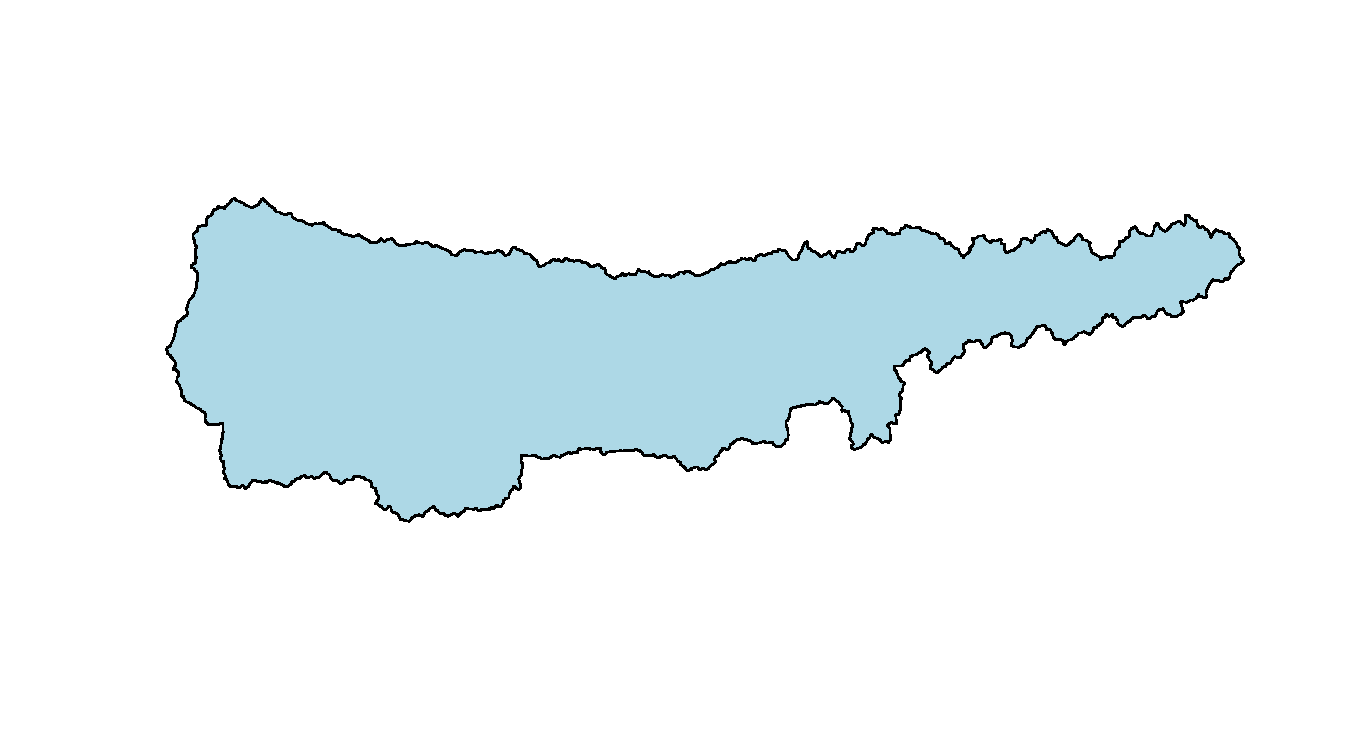
\includegraphics[width=.55\textwidth]{./externalfig/Zerafshan_shapefile_import.pdf}
\end{center}
\end{frame}

%------------------------------------------------------------%

\begin{frame}[fragile]\frametitle{shapefile with the central asian catchments I}
\begin{knitrout}\tiny
\definecolor{shadecolor}{rgb}{0.961, 0.961, 0.961}\color{fgcolor}\begin{kframe}
\begin{alltt}
\hlkwd{ogrListLayers}\hlstd{(}\hlstr{"data/GIS/ca_catchments.shp"}\hlstd{)}
\end{alltt}
\begin{verbatim}
## [1] "ca_catchments"
## attr(,"driver")
## [1] "ESRI Shapefile"
## attr(,"nlayers")
## [1] 1
\end{verbatim}
\begin{alltt}
\hlkwd{ogrInfo}\hlstd{(}\hlstr{"data/GIS/ca_catchments.shp"}\hlstd{,} \hlkwc{layer}\hlstd{=}\hlstr{"ca_catchments"}\hlstd{)}
\end{alltt}
\begin{verbatim}
## Source: "data/GIS/ca_catchments.shp", layer: "ca_catchments"
## Driver: ESRI Shapefile; number of rows: 25 
## Feature type: wkbPolygon with 2 dimensions
## Extent: (59.57317 33.67317) - (78.35566 43.0608)
## CRS: +proj=longlat +datum=WGS84 +no_defs  
## LDID: 87 
## Number of fields: 3 
##      name type length typeName
## 1      ID    0     10  Integer
## 2    NAME    4     30   String
## 3 PROCESS    0      4  Integer
\end{verbatim}
\end{kframe}
\end{knitrout}
\end{frame}

%------------------------------------------------------------%

\begin{frame}[fragile]\frametitle{shapefile with the central asian catchments II}
\begin{knitrout}\footnotesize
\definecolor{shadecolor}{rgb}{0.961, 0.961, 0.961}\color{fgcolor}\begin{kframe}
\begin{alltt}
\hlstd{cacatch} \hlkwb{<-} \hlkwd{readOGR}\hlstd{(}\hlstr{"data/GIS/ca_catchments.shp"}\hlstd{,}
                   \hlkwc{layer}\hlstd{=}\hlstr{"ca_catchments"}\hlstd{)}
\end{alltt}
\begin{verbatim}
## OGR data source with driver: ESRI Shapefile 
## Source: "data/GIS/ca_catchments.shp", layer: "ca_catchments"
## with 25 features
## It has 3 fields
\end{verbatim}
\end{kframe}
\end{knitrout}
\end{frame}

%------------------------------------------------------------%

\begin{frame}[fragile]\frametitle{shapefile with the central asian catchments III}
\begin{knitrout}\footnotesize
\definecolor{shadecolor}{rgb}{0.961, 0.961, 0.961}\color{fgcolor}\begin{kframe}
\begin{alltt}
\hlkwd{str}\hlstd{(cacatch,} \hlkwc{max.lev}\hlstd{=}\hlnum{2}\hlstd{)}
\end{alltt}
\begin{verbatim}
## Formal class 'SpatialPolygonsDataFrame' [package "sp"] with 5 slots
##   ..@ data       :'data.frame':	25 obs. of  3 variables:
##   ..@ polygons   :List of 25
##   ..@ plotOrder  : int [1:25] 9 11 14 2 21 13 20 16 12 8 ...
##   ..@ bbox       : num [1:2, 1:2] 59.6 33.7 78.4 43.1
##   .. ..- attr(*, "dimnames")=List of 2
##   ..@ proj4string:Formal class 'CRS' [package "sp"] with 1 slot
\end{verbatim}
\end{kframe}
\end{knitrout}
\end{frame}

%------------------------------------------------------------%

\begin{frame}[fragile]\frametitle{shapefile with the central asian catchments IV}
\begin{knitrout}
\definecolor{shadecolor}{rgb}{0.961, 0.961, 0.961}\color{fgcolor}\begin{kframe}
\begin{alltt}
\hlkwd{plot}\hlstd{(cacatch)}
\end{alltt}
\end{kframe}

{\centering \includegraphics[width=.8\textwidth]{./fig/Central_asia_shapefile_import4-1} 

}



\end{knitrout}
\end{frame}

%------------------------------------------------------------%

\begin{frame}[fragile]\frametitle{Shapefile: The river lines for the Zarafshan catchment}
% eval=TRUE
\begin{knitrout}\small
\definecolor{shadecolor}{rgb}{0.961, 0.961, 0.961}\color{fgcolor}\begin{kframe}
\begin{alltt}
\hlcom{# read a shapefile with the Zerafshan river}
\hlkwd{ogrListLayers}\hlstd{(}\hlstr{"data/GIS/Zerafshan_river_network.shp"}\hlstd{)}
\hlkwd{ogrInfo}\hlstd{(}\hlstr{"data/GIS/Zerafshan_river_network.shp"}\hlstd{,}
        \hlkwc{layer}\hlstd{=}\hlstr{"Zerafshan_river_network"}\hlstd{)}
\hlstd{zerriver} \hlkwb{<-} \hlkwd{readOGR}\hlstd{(}\hlstr{"data/GIS/Zerafshan_river_network.shp"}\hlstd{,}
                    \hlkwc{layer}\hlstd{=}\hlstr{"Zerafshan_river_network"}\hlstd{)}
\hlkwd{plot}\hlstd{(zerriver,} \hlkwc{add}\hlstd{=T,} \hlkwc{col}\hlstd{=}\hlstr{"darkblue"}\hlstd{)}
\end{alltt}
\end{kframe}
\end{knitrout}
\end{frame}

%------------------------------------------------------------%

\begin{frame}[fragile]\frametitle{Textfile: List of meteorological stations with coordinates}
\begin{knitrout}\footnotesize
\definecolor{shadecolor}{rgb}{0.961, 0.961, 0.961}\color{fgcolor}\begin{kframe}
\begin{alltt}
\hlcom{# read a textfile containing coordinates}
\hlstd{metstations} \hlkwb{<-} \hlkwd{read.table}\hlstd{(}\hlstr{"data/stationdata_10.dat"}\hlstd{)}
\hlkwd{str}\hlstd{(metstations,} \hlkwc{vec.len}\hlstd{=}\hlnum{2}\hlstd{)}
\end{alltt}
\begin{verbatim}
## 'data.frame':	226 obs. of  7 variables:
##  $ V1: int  1 2 3 4 5 ...
##  $ V2: num  43.5 44.1 ...
##  $ V3: num  68.9 75.8 ...
##  $ V4: num  9.69 -1.99 ...
##  $ V5: num  16.3 -13.1 ...
##  $ V6: int  697 566 3134 268 1607 ...
##  $ V7: Factor w/ 226 levels "ACISAJ","AHEQI",..: 1 3 4 7 9 ...
\end{verbatim}
\begin{alltt}
\hlkwd{colnames}\hlstd{(metstations)} \hlkwb{<-} \hlkwd{c}\hlstd{(}\hlstr{"INDEX"}\hlstd{,} \hlstr{"LAT"}\hlstd{,} \hlstr{"LONG"}\hlstd{,} \hlstr{"UN1"}\hlstd{,} \hlstr{"UN2"}\hlstd{,}
                           \hlstr{"UN3"}\hlstd{,} \hlstr{"STATION"}\hlstd{)}
\hlkwd{library}\hlstd{(sp)}
\hlkwd{coordinates}\hlstd{(metstations)} \hlkwb{<-} \hlopt{~} \hlstd{LONG} \hlopt{+} \hlstd{LAT}
\end{alltt}
\end{kframe}
\end{knitrout}
% zer.metstations <- point.in.polygon(metstations, 
% plot(metstations, add=T)
\end{frame}

%------------------------------------------------------------%

\begin{frame}[fragile]\frametitle{Ascii grid: The DEM for the Zarafshan catchment I}
% eval=TRUE
\begin{knitrout}
\definecolor{shadecolor}{rgb}{0.961, 0.961, 0.961}\color{fgcolor}\begin{kframe}
\begin{alltt}
\hlcom{# DEM of Zerafshan 500m resolution as background}
\hlstd{zerdem500} \hlkwb{<-} \hlkwd{readGDAL}\hlstd{(}\hlstr{"data/GIS/zerafshan_dem500m.asc"}\hlstd{)}
\hlkwd{image}\hlstd{(zerdem500,} \hlkwc{col}\hlstd{=}\hlkwd{terrain.colors}\hlstd{(}\hlnum{100}\hlstd{))}
\hlkwd{plot}\hlstd{(metstations,} \hlkwc{add}\hlstd{=T,} \hlkwc{col}\hlstd{=}\hlstr{"darkgrey"}\hlstd{)}
\hlkwd{plot}\hlstd{(zercatch,} \hlkwc{add}\hlstd{=T,} \hlkwc{lwd}\hlstd{=}\hlnum{2}\hlstd{)}
\hlkwd{plot}\hlstd{(zerriver,} \hlkwc{col}\hlstd{=}\hlstr{"blue"}\hlstd{,} \hlkwc{add}\hlstd{=T)}
\end{alltt}
\end{kframe}
\end{knitrout}
\end{frame}

%------------------------------------------------------------%

\begin{frame}[fragile]\frametitle{Ascii grid: The DEM for the Zarafshan catchment II}
\begin{center}
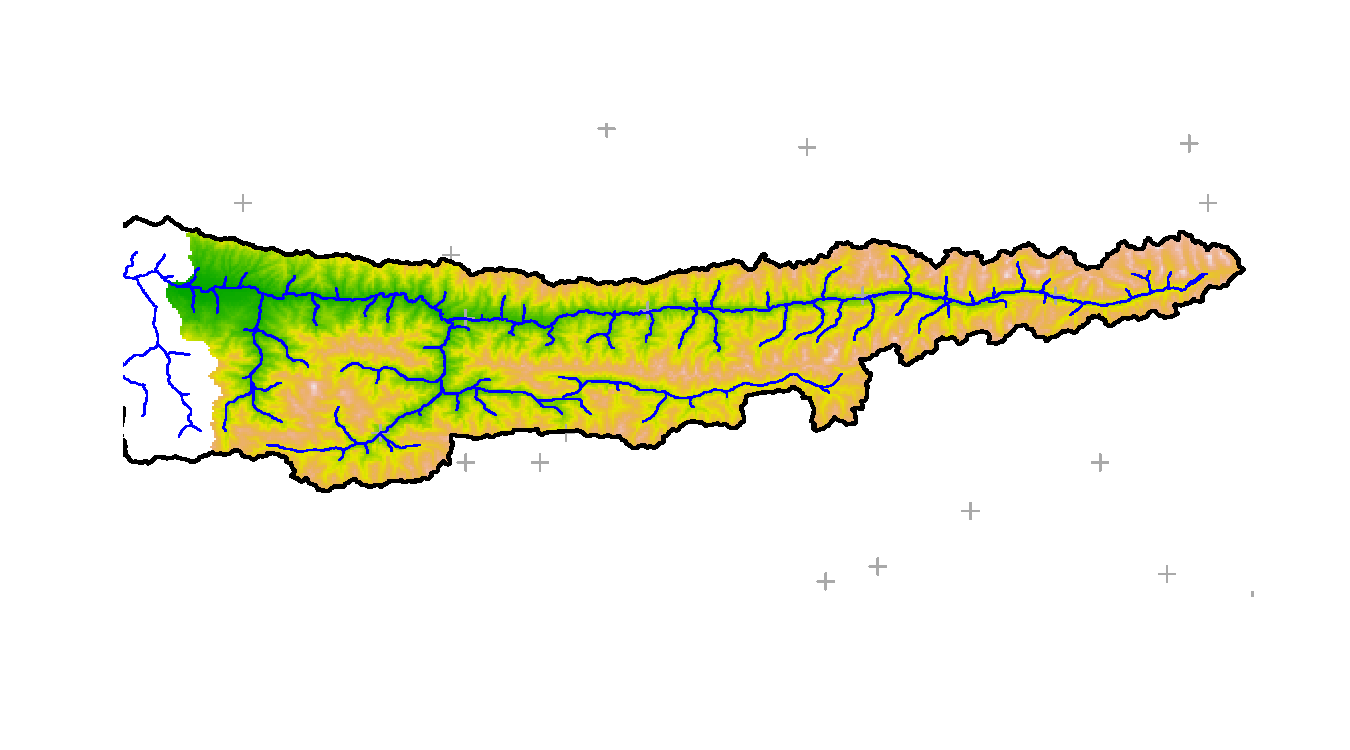
\includegraphics[width=0.96\textwidth]{./externalfig/Zerafshan_DEM_import1.pdf}
\end{center}
\end{frame}

%------------------------------------------------------------%

\begin{frame}[fragile]\frametitle{Plotting with basic commands}
\begin{knitrout}
\definecolor{shadecolor}{rgb}{0.961, 0.961, 0.961}\color{fgcolor}\begin{kframe}
\begin{alltt}
\hlkwd{image}\hlstd{(zerdem500,} \hlkwc{col}\hlstd{=}\hlkwd{terrain.colors}\hlstd{(}\hlnum{100}\hlstd{))}
\hlkwd{plot}\hlstd{(metstations,} \hlkwc{add}\hlstd{=T,} \hlkwc{col}\hlstd{=}\hlstr{"darkgrey"}\hlstd{)}
\hlkwd{plot}\hlstd{(zercatch,} \hlkwc{add}\hlstd{=T,} \hlkwc{lwd}\hlstd{=}\hlnum{2}\hlstd{)}
\hlkwd{plot}\hlstd{(zerriver,} \hlkwc{col}\hlstd{=}\hlstr{"blue"}\hlstd{,} \hlkwc{add}\hlstd{=T)}
\end{alltt}
\end{kframe}
\end{knitrout}
\begin{center}
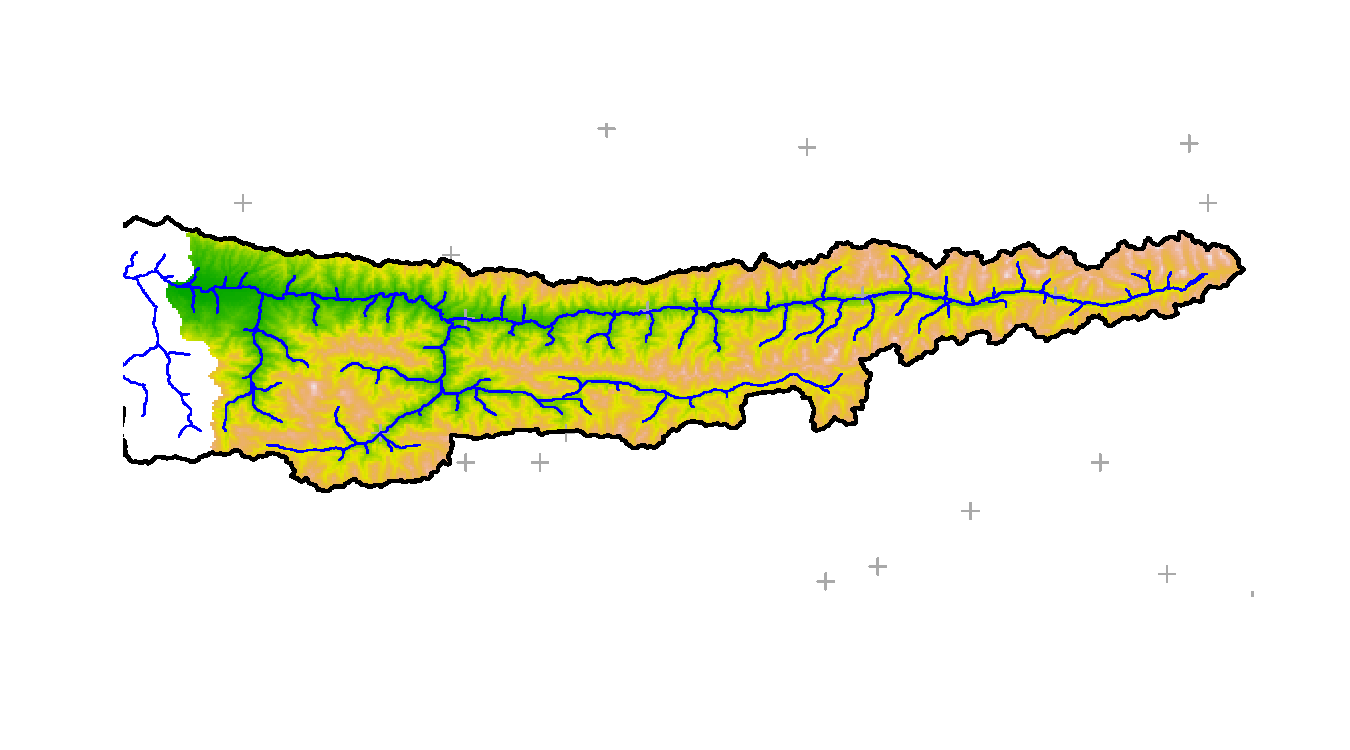
\includegraphics[width=0.75\textwidth]{./externalfig/basic_plotting.pdf}
\end{center}
\end{frame}

%------------------------------------------------------------%

% # read country boundaries
% load("data/GIS/GADM/KGZ_adm0.RData")
% kgz0 <- gadm
% plot(kgz0, add=T)
% load("data/GIS/GADM/TJK_adm0.RData")
% tjk0 <- gadm
% plot(tjk0, add=T)
% load("data/GIS/GADM/KAZ_adm0.RData")
% kaz0 <- gadm
% plot(kaz0, add=T)
% load("data/GIS/GADM/UZB_adm0.RData")
% uzb0 <- gadm
% plot(uzb0, add=T)

%------------------------------------------------------------%

\begin{frame}[fragile]\frametitle{Plotting with \rcode{spplot}}
% eval=TRUE
\begin{knitrout}
\definecolor{shadecolor}{rgb}{0.961, 0.961, 0.961}\color{fgcolor}\begin{kframe}
\begin{alltt}
\hlcom{# prepare an spplot}
\hlkwd{spplot}\hlstd{(zerdem500)}
\end{alltt}
\end{kframe}
\end{knitrout}
\begin{center}
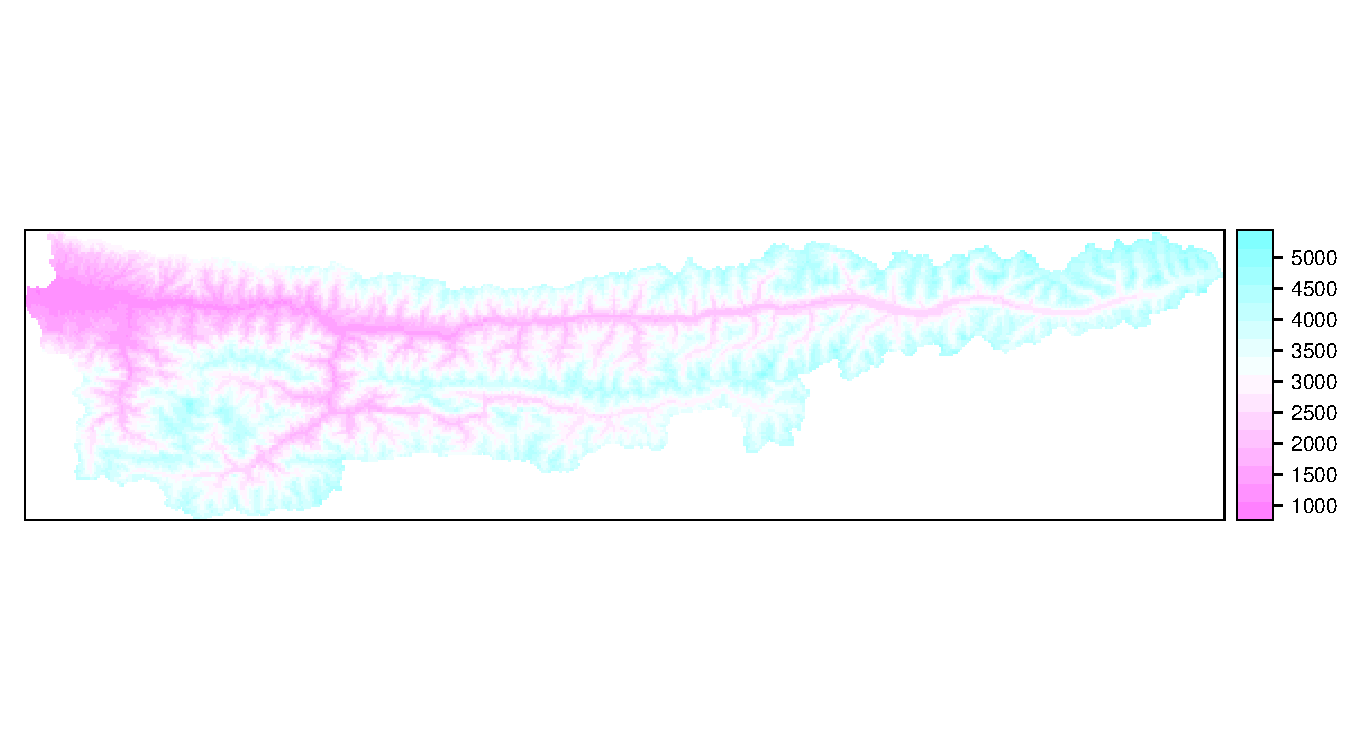
\includegraphics[width=0.9\textwidth]{./externalfig/advanced_plotting_with_standard_spplot.pdf}
\end{center}
\end{frame}

%------------------------------------------------------------%

\begin{frame}[fragile]\frametitle{Plotting with \rcode{spplot}}
% eval=TRUE
\begin{knitrout}\scriptsize
\definecolor{shadecolor}{rgb}{0.961, 0.961, 0.961}\color{fgcolor}\begin{kframe}
\begin{alltt}
\hlcom{# prepare a spplot}
\hlstd{spl.zercatch} \hlkwb{<-} \hlkwd{list}\hlstd{(}\hlstr{"sp.polygons"}\hlstd{,} \hlkwc{first}\hlstd{=F, zercatch,} \hlkwc{col}\hlstd{=}\hlstr{"lightblue"}\hlstd{,} \hlkwc{lwd}\hlstd{=}\hlnum{2}\hlstd{)}
\hlstd{spl.zerriver} \hlkwb{<-} \hlkwd{list}\hlstd{(}\hlstr{"sp.lines"}\hlstd{,} \hlkwc{first}\hlstd{=F,} \hlkwc{col}\hlstd{=}\hlkwd{addAlpha}\hlstd{(}\hlstr{"blue"}\hlstd{,}\hlnum{0.7}\hlstd{), zerriver)}
\hlstd{spl.stat} \hlkwb{<-} \hlkwd{list}\hlstd{(}\hlstr{"sp.points"}\hlstd{,} \hlkwc{first}\hlstd{=F,} \hlkwc{col}\hlstd{=}\hlstr{"grey20"}\hlstd{, metstations)}
\hlstd{spl.text} \hlkwb{<-} \hlkwd{list}\hlstd{(}\hlstr{"sp.text"}\hlstd{,} \hlkwc{first}\hlstd{=F,} \hlkwc{col}\hlstd{=}\hlstr{"grey20"}\hlstd{,} \hlkwc{loc}\hlstd{=}\hlkwd{coordinates}\hlstd{(metstations),}
                 \hlkwc{txt}\hlstd{=metstations}\hlopt{$}\hlstd{STATION,} \hlkwc{cex}\hlstd{=}\hlnum{0.7}\hlstd{,} \hlkwc{adj}\hlstd{=}\hlnum{1}\hlstd{)}
\end{alltt}
\end{kframe}
\end{knitrout}
\onslide<2>
Transparency of colors: addAlpha in these slides is referring to 
\begin{knitrout}
\definecolor{shadecolor}{rgb}{0.961, 0.961, 0.961}\color{fgcolor}\begin{kframe}
\begin{alltt}
\hlkwd{install.packages}\hlstd{(}\hlstr{"berryFunctions"}\hlstd{)}
\hlkwd{library}\hlstd{(berryFunctions)}
\hlopt{?}\hlstd{addAlpha}
\end{alltt}
\end{kframe}
\end{knitrout}
\end{frame}

%------------------------------------------------------------%

\begin{frame}[fragile]\frametitle{Plotting with \rcode{spplot}}
% eval=TRUE
\begin{knitrout}
\definecolor{shadecolor}{rgb}{0.961, 0.961, 0.961}\color{fgcolor}\begin{kframe}
\begin{alltt}
\hlcom{# prepare a spplot}
\hlkwd{spplot}\hlstd{(zerdem500,} \hlkwc{scales}\hlstd{=}\hlkwd{list}\hlstd{(}\hlkwc{draw}\hlstd{=T),}
       \hlkwc{col.regions}\hlstd{=}\hlkwd{addAlpha}\hlstd{(}\hlkwd{terrain.colors}\hlstd{(}\hlnum{200}\hlstd{),} \hlnum{0.6}\hlstd{),}
       \hlkwc{sp.layout}\hlstd{=}\hlkwd{list}\hlstd{(spl.zercatch, spl.zerriver,}
                      \hlstd{spl.stat, spl.text, spl.scale))}
\end{alltt}
\end{kframe}
\end{knitrout}
\end{frame}

%------------------------------------------------------------%

% ascii raster
% <<asciiraster>>=
% library(rgdal)
% GDALinfo("data/GIS/MODIS/karadarya/2013/Step8//2013003_cloud_free.asc")
% modis2013.3 <- readGDAL("data/GIS/MODIS/karadarya/2013/Step8//2013003_cloud_free.asc")
% str(modis2013.3)
% @


%------------------------------------------------------------%
%------------------------------------------------------------%
\subsection{Visualising spatial data}
%------------------------------------------------------------%
%------------------------------------------------------------%

\begin{frame}[fragile]\frametitle{Overlay: visual - using compound plot functions}
For plotting we can use the \rcode{sp} functionality
\begin{knitrout}
\definecolor{shadecolor}{rgb}{0.961, 0.961, 0.961}\color{fgcolor}\begin{kframe}
\begin{alltt}
\hlkwd{library}\hlstd{(sp)}
\hlkwd{demo}\hlstd{(meuse)}
\hlstd{size} \hlkwb{=} \hlstd{meuse}\hlopt{$}\hlstd{zinc} \hlopt{/} \hlkwd{mean}\hlstd{(meuse}\hlopt{$}\hlstd{zinc)}
\hlstd{pts} \hlkwb{=} \hlkwd{list}\hlstd{(}\hlstr{"sp.points"}\hlstd{, meuse,} \hlkwc{pch} \hlstd{=} \hlnum{1}\hlstd{,} \hlkwc{cex} \hlstd{= size)}
\hlstd{riv} \hlkwb{=} \hlkwd{list}\hlstd{(}\hlstr{"sp.polygons"}\hlstd{, meuse.riv)}
\hlstd{plt} \hlkwb{=} \hlkwd{spplot}\hlstd{(meuse.grid[}\hlstr{"dist"}\hlstd{],} \hlkwc{sp.layout}\hlstd{=}\hlkwd{list}\hlstd{(pts, riv))}
\hlkwd{class}\hlstd{(plt)}
\end{alltt}
\end{kframe}
\end{knitrout}
\end{frame}

%------------------------------------------------------------%

\begin{frame}[fragile]\frametitle{Overlay: visual - using compound plot functions}
\begin{knitrout}
\definecolor{shadecolor}{rgb}{0.961, 0.961, 0.961}\color{fgcolor}\begin{kframe}
\begin{alltt}
\hlkwd{print}\hlstd{(plt)}
\end{alltt}
\end{kframe}
\end{knitrout}
\begin{center}
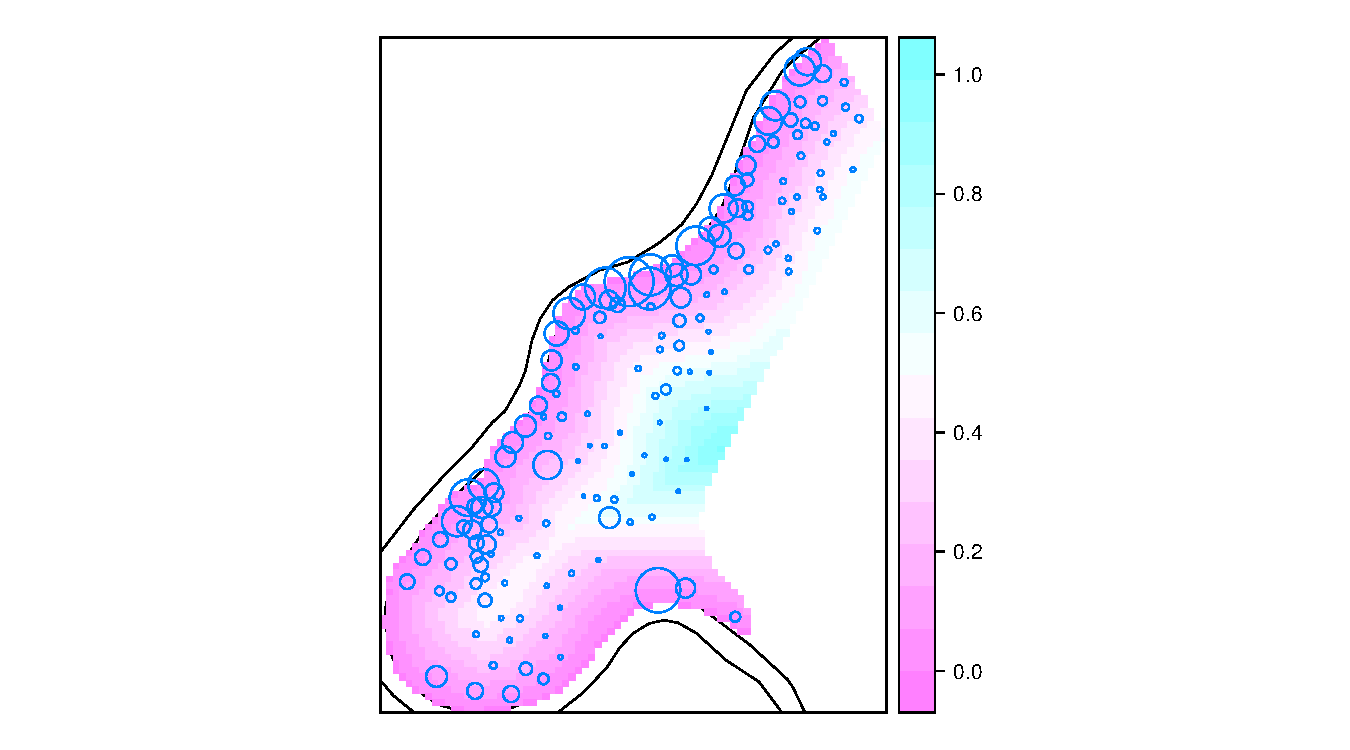
\includegraphics[width=0.9\textwidth]{./externalfig/Plotting_with_the_sp_package_print.pdf}
\end{center}
\end{frame}

%------------------------------------------------------------%

\begin{frame}[fragile]\frametitle{Cartography?}
\pause
\begin{itemize}[<+->]
\item A map is a plot with longitude and latitude, and a controlled aspect ratio; 
\item any plotting software can "do" maps, however
\item reference comes from coast lines, rivers, lakes, topography, political boundaries, cities, land use etc.
\item reference grid lines (parallels, meridians) may be required, and be non-straight
\item axes tics usually show little, but some information
\item custom elements are often present (arrow, scale bar, multi-type legend)
\item label placement is challenging (but see: \rcode{rgeos::polyLabel})
\end{itemize}
\end{frame}

%------------------------------------------------------------%

\begin{frame}[fragile]\frametitle{Plot example: Overlaying a grid with polygons to give the viewer reference}
from some of my work I brought the following
\pause
\begin{itemize}[<+->]
\item gridded monthly drought composites of sea surface temperature anomalies in the Limpopo basin (Southern Africa)
\item country border and continent polygons
\item river and catchment
\end{itemize}
\end{frame}

%------------------------------------------------------------%

\begin{frame}[fragile]\frametitle{The El Nino phenomenon}
  El Nino is an anomaly of sea surface temperatures in the Pacific. It is related to climate anomalies around the globe.
  \begin{figure}[h]
    \begin{center}
    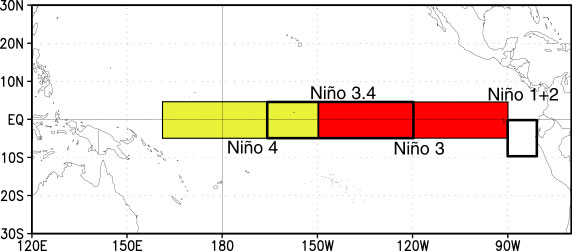
\includegraphics[width=.8\linewidth]{./externalfig/ninoareas_c.jpg}
    \caption{El nino southern Oscillation (ENSO) regions (NOAA webpage).}
  	\label{fig:ensoreg}
    \end{center}
	\end{figure}
\end{frame}

%------------------------------------------------------------%

\begin{frame}[fragile]\frametitle{Calculating composites}
The purpose of composites is to identify anomalies in meteorological data that are associated to an specific pattern or an unusual occurence (p.g. extreme events). Here:
\pause
\begin{itemize}[<+->]
\item Times were identified at which there was a drought in the Limpopo basin
\item Sea surface temperatures in the surrounding oceans were averaged for these times
\item anomalies were tested for significance (were there deviations from non-drought times?)
\end{itemize}
\end{frame}

%------------------------------------------------------------%

\begin{frame}[fragile]\frametitle{Composite example plot}
\begin{knitrout}\small
\definecolor{shadecolor}{rgb}{0.961, 0.961, 0.961}\color{fgcolor}\begin{kframe}
\begin{alltt}
\hlcom{# the was saved as Rdata}
\hlkwd{load}\hlstd{(}\hlstr{"data/GIS/composites/comp2_HydD_Limpopo_HadISST.Rdata"}\hlstd{)}
\hlkwd{class}\hlstd{(c2sst)}
\end{alltt}
\begin{verbatim}
## [1] "STFDF"
## attr(,"package")
## [1] "spacetime"
\end{verbatim}
\begin{alltt}
\hlcom{# one composite per month}

\hlkwd{library}\hlstd{(spacetime)}
\hlkwd{suppressMessages}\hlstd{(} \hlkwd{library}\hlstd{(zoo) )}
\end{alltt}
\end{kframe}
\end{knitrout}
\end{frame}

%------------------------------------------------------------%

\begin{frame}[fragile]\frametitle{Composite example plot}
\begin{knitrout}
\definecolor{shadecolor}{rgb}{0.961, 0.961, 0.961}\color{fgcolor}\begin{kframe}
\begin{alltt}
\hlcom{# There was one composite per month}
\hlcom{# convert data to a SpatialPixelsDataFrame}
\hlstd{c2sst.HD} \hlkwb{<-} \hlkwd{as}\hlstd{(c2sst,} \hlstr{"Spatial"}\hlstd{)}
\hlkwd{class}\hlstd{(c2sst.HD)}
\end{alltt}
\begin{verbatim}
## [1] "SpatialPixelsDataFrame"
## attr(,"package")
## [1] "sp"
\end{verbatim}
\begin{alltt}
\hlcom{# change column names (you recognise the functions?!)}
\hlkwd{names}\hlstd{(c2sst.HD)} \hlkwb{<-} \hlkwd{format}\hlstd{(}\hlkwd{time}\hlstd{(c2sst),} \hlstr{"%B"}\hlstd{)}
\end{alltt}
\end{kframe}
\end{knitrout}
\end{frame}

%------------------------------------------------------------%

\begin{frame}[fragile]\frametitle{Composite example plot}
\begin{knitrout}
\definecolor{shadecolor}{rgb}{0.961, 0.961, 0.961}\color{fgcolor}\begin{kframe}
\begin{alltt}
\hlkwd{spplot}\hlstd{(c2sst.HD)}
\end{alltt}
\end{kframe}

{\centering \includegraphics[width=.8\textwidth]{./fig/plain_composite_plot-1} 

}



\end{knitrout}
\end{frame}

%------------------------------------------------------------%

\begin{frame}[fragile]\frametitle{Composite example plot}
For reference we want to plot the continent outlines and the Limpopo basin on top of the composite grid
\begin{knitrout}\small
\definecolor{shadecolor}{rgb}{0.961, 0.961, 0.961}\color{fgcolor}\begin{kframe}
\begin{alltt}
\hlkwd{library}\hlstd{(maps)}
\hlkwd{suppressMessages}\hlstd{(}  \hlkwd{library}\hlstd{(maptools)  )}
\hlcom{# create a world map}
\hlstd{worldb} \hlkwb{<-} \hlkwd{map}\hlstd{(}\hlstr{'world'}\hlstd{,} \hlkwc{interior}\hlstd{=F,} \hlkwc{plot}\hlstd{=F,} \hlkwc{fill}\hlstd{=T,}
              \hlkwc{col}\hlstd{=}\hlstr{"transparent"}\hlstd{)}
\hlcom{# convert it to the necessary SpatialPolygons class}
\hlstd{IDs} \hlkwb{<-} \hlkwd{sapply}\hlstd{(}\hlkwd{strsplit}\hlstd{(worldb}\hlopt{$}\hlstd{names,} \hlstr{":"}\hlstd{),} \hlstr{"["}\hlstd{,} \hlnum{1}\hlstd{)}
\hlstd{worldb} \hlkwb{<-} \hlkwd{map2SpatialPolygons}\hlstd{(worldb,} \hlkwc{ID}\hlstd{=IDs,}
          \hlkwc{proj4string}\hlstd{=}\hlkwd{CRS}\hlstd{(}\hlstr{"+proj=longlat +datum=WGS84"}\hlstd{))}
\hlkwd{class}\hlstd{(worldb)}
\end{alltt}
\begin{verbatim}
## [1] "SpatialPolygons"
## attr(,"package")
## [1] "sp"
\end{verbatim}
\end{kframe}
\end{knitrout}
\end{frame}

%------------------------------------------------------------%

\begin{frame}[fragile]\frametitle{Composite example plot}
\begin{knitrout}\tiny
\definecolor{shadecolor}{rgb}{0.961, 0.961, 0.961}\color{fgcolor}\begin{kframe}
\begin{alltt}
\hlkwd{ogrListLayers}\hlstd{(}\hlstr{"data/GIS/HYDROSHEDS_Limpopo_catchment.shp"}\hlstd{)}
\end{alltt}
\begin{verbatim}
## [1] "HYDROSHEDS_Limpopo_catchment"
## attr(,"driver")
## [1] "ESRI Shapefile"
## attr(,"nlayers")
## [1] 1
\end{verbatim}
\begin{alltt}
\hlkwd{ogrInfo}\hlstd{(}\hlstr{"data/GIS/HYDROSHEDS_Limpopo_catchment.shp"}\hlstd{,} \hlkwc{layer}\hlstd{=}\hlstr{"HYDROSHEDS_Limpopo_catchment"}\hlstd{)}
\end{alltt}
\begin{verbatim}
## Source: "data/GIS/HYDROSHEDS_Limpopo_catchment.shp", layer: "HYDROSHEDS_Limpopo_catchment"
## Driver: ESRI Shapefile; number of rows: 1 
## Feature type: wkbPolygon with 2 dimensions
## Extent: (25.125 -26.52083) - (34.42917 -19.76667)
## CRS: +proj=longlat +datum=WGS84 +no_defs  
## LDID: 87 
## Number of fields: 2 
##        name type length typeName
## 1  BASIN_ID    0     10  Integer
## 2 AREA_SQKM    2     12     Real
\end{verbatim}
\end{kframe}
\end{knitrout}
\end{frame}

%------------------------------------------------------------%

\begin{frame}[fragile]\frametitle{Composite example plot}
\begin{knitrout}\tiny
\definecolor{shadecolor}{rgb}{0.961, 0.961, 0.961}\color{fgcolor}\begin{kframe}
\begin{alltt}
\hlstd{limpopocatch} \hlkwb{<-} \hlkwd{readOGR}\hlstd{(}\hlstr{"data/GIS/HYDROSHEDS_Limpopo_catchment.shp"}\hlstd{,}
                        \hlkwc{layer}\hlstd{=}\hlstr{"HYDROSHEDS_Limpopo_catchment"}\hlstd{)}
\end{alltt}
\begin{verbatim}
## OGR data source with driver: ESRI Shapefile 
## Source: "data/GIS/HYDROSHEDS_Limpopo_catchment.shp", layer: "HYDROSHEDS_Limpopo_catchment"
## with 1 features
## It has 2 fields
\end{verbatim}
\end{kframe}
\end{knitrout}
\end{frame}
%------------------------------------------------------------%

\begin{frame}[fragile]\frametitle{Composite example plot}
We build up the plot layer by layer by specifying  sp.layout
% eval=TRUE
\begin{knitrout}
\definecolor{shadecolor}{rgb}{0.961, 0.961, 0.961}\color{fgcolor}\begin{kframe}
\begin{alltt}
\hlstd{sp.layout} \hlkwb{<-} \hlkwd{list}\hlstd{(}
  \hlkwd{list}\hlstd{(}\hlstr{"sp.polygons"}\hlstd{, worldb,} \hlkwc{first}\hlstd{=F,}
       \hlkwc{col}\hlstd{=}\hlstr{"grey80"}\hlstd{,} \hlkwc{fill}\hlstd{=}\hlstr{"grey80"}\hlstd{),}
  \hlkwd{list}\hlstd{(}\hlstr{"sp.polygons"}\hlstd{, limpopocatch,} \hlkwc{first}\hlstd{=F,}
       \hlkwc{col}\hlstd{=}\hlstr{"grey60"}\hlstd{,} \hlkwc{fill}\hlstd{=}\hlstr{"transparent"}\hlstd{)}
\hlstd{)}
\end{alltt}
\end{kframe}
\end{knitrout}
\end{frame}

%------------------------------------------------------------%

\begin{frame}[fragile]\frametitle{Composite example plot}
Finally, plot the designed maps
\begin{knitrout}
\definecolor{shadecolor}{rgb}{0.961, 0.961, 0.961}\color{fgcolor}\begin{kframe}
\begin{alltt}
\hlkwd{spplot}\hlstd{(c2sst.HD,} \hlkwc{sp.layout}\hlstd{=sp.layout,} \hlkwc{scales}\hlstd{=}\hlkwd{list}\hlstd{(}\hlkwc{draw}\hlstd{=T))}
\end{alltt}
\end{kframe}
\end{knitrout}
% This takes long, so I set eval=FALSE after ther first time
\begin{center}
\includegraphics[width=0.9\textwidth]{./fig/plot_the_composites_with_overlaid_layers.pdf}
\end{center}
\end{frame}

%------------------------------------------------------------%

\begin{frame}[fragile]\frametitle{Your turn ...}
This is R programming for experienced users, so take some time and try to understand the example.
\begin{exercise}{Create the same plot with the provided data set (\small{\texttt{data/GIS/composites/comp2\_HydD\_ELNINO\_Limpopo\_HadISST.Rdata}})} %ex21
\begin{enumerate}
\item \rcode{load} the new data set 
\item Plot it by using the code provided above
\item Check the help on \rcode{spplot} and plot "May" only
\item Adjust the color of the superimposed catchment outline and give it a blue touch.
\end{enumerate}
\end{exercise}
\end{frame}

%------------------------------------------------------------%

% \begin{frame}[fragile]\frametitle{Solution for exercise \arabic{exercisecount}.1}
% <<ex19sola, eval=FALSE>>=
% # ToDo
% @
% \end{frame}

%------------------------------------------------------------%

% EDZER
% Cartography?

%------------------------------------------------------------%

\begin{frame}[fragile]\frametitle{What is R good at?}
\pause
\begin{itemize}[<+->]
\item repetitive graphs:
  \begin{itemize}
  \item many, similar graphs, over different pages
  \item many graphs combined in a lattice (grid: lattice, ggplot)
  \end{itemize}
\item non-interactive, reproducible use
\item control of all details
\item richness of graphics devices,
\item portability, cross-platform, options for deployment
\end{itemize}
\end{frame}

%------------------------------------------------------------%

\begin{frame}[fragile]\frametitle{What is R bad at?}
\pause
\begin{itemize}[<+->]
\item interactive use: zoom, pan, edit graph element etc.
\item control is not trivial
\item incompatible plotting systems: base, lattice, ggplot, ...
\end{itemize}
\end{frame}

%------------------------------------------------------------%

% own example of overlays with polygons, grid and more

%------------------------------------------------------------%
%------------------------------------------------------------%
% \subsection{More methods for spatial data}
%------------------------------------------------------------%
%------------------------------------------------------------%

% methods for spatial classes
% outlook: gstat with meuse kriging and so on

% EDZER
% Two work horses: rgdal, rgeos
% library(rgdal);  library(rgeos)
% rgdal links to the GDAL (raster) and OGR (vector) data I/O library, as well as PROJ.4 for CRS (coordinate reference systems) (re)projections
% rgeos links to the GEOS (Geometry Open Source) library, which powers PostGIS: does the \usual"geometry operations for features

% What is numerical overlay?
% Method over(x,y) provides: consistent spatial overlay for points, grids, lines and polygons
% at the spatial locations of object x, retrieve the indexes or attributes from spatial object y and NA in case of no match (index vector if y has only geometry, attribute data.frame if it has attributes too).
% library(sp); loadMeuse()
% over(meuse, geometry(meuse.grid))[1:10]
% over(meuse, meuse.grid)[1:3,]
% In SQL, this resembles a left outer join of two tables

% Aggregation, the R way, for a data.frame, based on a table column:
% m = as(meuse, "data.frame")[c("zinc", "lead")]
% aggregate(m, by = list(ffreq = meuse$ffreq), mean)
% # create a coarse grid:
% off = gridparameters(meuse.grid)$cellcentre.offset + 20
% gt = GridTopology(off, c(400,400), c(8,11))
% SG = SpatialGrid(gt)
% proj4string(SG) = proj4string(meuse.grid)
% # for a Spatial object, based on another Spatial object:
% agg = aggregate(meuse[c("zinc","lead")], SG, FUN = mean)
% spplot(agg, sp.layout = pts)

% Which pixels are covered by points? Selection with over
% SP = as(SG, "SpatialPolygons")
% over(SP, geometry(meuse))
% length(SP[!is.na(over(SP, geometry(meuse)))])
% length(SP[meuse]) # equivalent!
% plot(as(SP[meuse], "SpatialPolygons"))
% points(meuse, col = 'red')

% raster package

% Open street maps: osmar
% library(osmar)
% api = osmsource_api()
% pt = c(7.609983,51.940812) # ifgi
% size = 0.005
% bb = do.call(corner_bbox, as.list(c(pt - size, pt + size)))
% ifgi = get_osm(bb, source = api)
% plot(ifgi)
% dx = c(-1, 1, 1, -1, -1)
% dy = c(-1, -1, 1, 1, -1)
% lines(pt[1] + dx * size, pt[2] + dy * size, col = 'red')
% lapply(as_sp(ifgi), class)
% class(as_igraph(ifgi))
% seems to give access to all vector data, in sp or igraph0 format!
% more openstreetmap eyecandy here:
% http://www.r-bloggers.com/the-openstreetmap-package-opens-up/

% block kriging example

% create a map  showing the outlines of Afghanistan and Pakistan
% library(maps)
% library(maptools)
% map("worldHires")
% map("worldHires", regions=c("Afghanistan", "Pakistan", "Tajikistan", "Kyrgystan", "Iran"), interior=T) # very embarassing: data is from before 1991
% map('rivers', add=TRUE, col="blue")
% ?worldHires

% plot of composites to show plotting capabilities with lattice
% quicker with maptools
% limpopocatch <-  readShapePoly ("data/GIS/HYDROSHEDS_Limpopo_catchment.shp", proj4string=CRS("+proj=longlat +datum=WGS84"))
% limpopo.river <- readShapeLines("data/GIS/HYDROSHEDS_Limpopo_river.shp",     proj4string=CRS("+proj=longlat +datum=WGS84"))

% example: plotting GADM Zimbabwe with Limpopo ERA I DI as background
% prepare data by reducing stfdf.limpopo to one SpatialGridDataFrame

% exercise: Download Rdata from GADM for central asia and plot dem with boundaries on top
% read dem
% read GADM
% merging of all polygons to one?
% plot all

% read prepared MODIS
% try to understand the report function
%source("F:/matsei/Documents/R/Introduction to R//R-Course_Bischkek/original_data//Material_Abror/R_Kurs//modsnow/skripte/modsnow_functions.R")
% impossible

% read dem
% read catchment 
% zerafshan
% Karadarya (MODIS available)
% Naryn (MODIS available)
% clip dem for a catchment
% add stations
% read modis
% Karadarya
% Naryn
% plot: overlay dem with snow data
% setwd("~/Documents/R/R-Course_Bischkek/original_data/Material_Abror/R_Kurs/modsnow/output/karadarya/2013/Step8")
% library(rgdal)


%------------------------------------------------------------%
%------------------------------------------------------------%
\subsection{Handling spatiotemporal data}
%------------------------------------------------------------%
%------------------------------------------------------------%

% spacetime package: classes, plotting, aggregation, animation

%------------------------------------------------------------%

\begin{frame}[fragile]\frametitle{Great vignettes to get started with the \texttt{spacetime} package}
\begin{knitrout}
\definecolor{shadecolor}{rgb}{0.961, 0.961, 0.961}\color{fgcolor}\begin{kframe}
\begin{alltt}
\hlkwd{library}\hlstd{(spacetime)}
\end{alltt}
\end{kframe}
\end{knitrout}
Vignettes on:
\pause
\begin{itemize}[<+->]
\item spacetime: Spatio-Temporal Data in R
\begin{knitrout}
\definecolor{shadecolor}{rgb}{0.961, 0.961, 0.961}\color{fgcolor}\begin{kframe}
\begin{alltt}
\hlkwd{vignette}\hlstd{(}\hlstr{"jss816"}\hlstd{,} \hlkwc{package}\hlstd{=}\hlstr{"spacetime"}\hlstd{)}
\end{alltt}
\end{kframe}
\end{knitrout}
\item Spatio-temporal overlay and aggregation
\begin{knitrout}
\definecolor{shadecolor}{rgb}{0.961, 0.961, 0.961}\color{fgcolor}\begin{kframe}
\begin{alltt}
\hlkwd{vignette}\hlstd{(}\hlstr{"sto"}\hlstd{,} \hlkwc{package}\hlstd{=}\hlstr{"spacetime"}\hlstd{)}
\end{alltt}
\end{kframe}
\end{knitrout}
\end{itemize}
\end{frame}

%------------------------------------------------------------%

% example of MODIS 

%------------------------------------------------------------%

\begin{frame}[fragile]\frametitle{Layouts for spatiotemporal data in \texttt{spacetime}}
\begin{center}
\includegraphics[width=0.6\textwidth]{./externalfig/spacetime_layouts.png}
\end{center}
\end{frame}


%------------------------------------------------------------%
%------------------------------------------------------------%
\end{document}
%------------------------------------------------------------%
%------------------------------------------------------------%

